% Appendices
\begin{appendices}
    \section{Input data}
        \subsection{Drum and cymbal classification}
        \label{app:classification}
        \texttt{Referred to in section \ref{sec:labelling_and_encoding}}\smallskip
        
        In \textit{settings.json} the type of hits, kit components and techniques used are described by the \textit{label} associative array. The combinations of these types which are valid classes are described by the  \textit{label-hierarchy} associative array. Here is the section of this file where they appear:
        
        \begin{lstlisting}
        "label": {
            "hit_label": ["beater", "stick"],
            "kit_label": [
              "bass_drum",
              "crash",
              "hi_hat",
              "high_tom",
              "mid_tom",
              "low_tom",
              "ride",
              "snare",
              "splash"
            ],
            "tech_label": ["bell", "normal", "open"]
        },
          
        "label-hierarchy": {
            "beater": { "bass_drum": ["normal"] },
            "stick": {
              "crash": ["normal"],
              "hi_hat": ["normal", "open"],
              "high_tom": ["normal"],
              "mid_tom": ["normal"],
              "low_tom": ["normal"],
              "ride": ["normal", "bell"],
              "snare": ["normal"]
            }
        }
        \end{lstlisting}
        
        Later the splash cymbal wasn't used because there wasn't enough raw data for it. Hence it doesn't appear in \textit{label-hierarchy} even though its still in \textit{label}.
        
        \newpage
        \subsection{Drum kit combinations}
        \label{app:kit-combinations}
        \texttt{Referred to in section \ref{sec:labelling_and_encoding}}\smallskip
        
        There are 87 different combinations of drum and cymbal that can be hit at once, since all drums and cymbals are hand operated apart from the bass drum and opening/closing hi-hat (not counting the hi-hat closing shut as a hit). The following list is how encodings were ordered:
        \begin{figure}[H]
            \centering
            \begin{tiny}
                \begin{tabular}{r|l|l|l|}
                    Index & \multicolumn{3}{c|}{Drum kit classes}\\
                    \hline
                    1 & bass-drum normal & & \\
                    \hline
                    2 & crash normal & & \\
                    \hline
                    3 & hi-hat normal & & \\
                    \hline
                    4 & hi-hat open & & \\
                    \hline
                    5 & high-tom normal & & \\
                    \hline
                    6 & low-tom normal & & \\
                    \hline
                    7 & mid-tom normal & & \\
                    \hline
                    8 & ride bell & & \\
                    \hline
                    9 & ride normal & & \\
                    \hline
                    10 & snare normal & & \\
                    \hline
                    11 & bass-drum normal & crash normal & \\
                    \hline
                    12 & bass-drum normal & hi-hat normal & \\
                    \hline
                    13 & bass-drum normal & hi-hat open & \\
                    \hline
                    14 & bass-drum normal & high-tom normal & \\
                    \hline
                    15 & bass-drum normal & low-tom normal & \\
                    \hline
                    16 & bass-drum normal & mid-tom normal & \\
                    \hline
                    17 & bass-drum normal & ride bell & \\
                    \hline
                    18 & bass-drum normal & ride normal & \\
                    \hline
                    19 & bass-drum normal & snare normal & \\
                    \hline
                    20 & crash normal & hi-hat normal & \\
                    \hline
                    21 & crash normal & hi-hat open & \\
                    \hline
                    22 & crash normal & high-tom normal & \\
                    \hline
                    23 & crash normal & low-tom normal & \\
                    \hline
                    24 & crash normal & mid-tom normal & \\
                    \hline
                    25 & crash normal & ride bell & \\
                    \hline
                    26 & crash normal & ride normal & \\
                    \hline
                    27 & crash normal & snare normal & \\
                    \hline
                    28 & hi-hat normal & high-tom normal & \\
                    \hline
                    29 & hi-hat normal & low-tom normal & \\
                    \hline
                    30 & hi-hat normal & mid-tom normal & \\
                    \hline
                    31 & hi-hat normal & ride bell & \\
                    \hline
                    32 & hi-hat normal & ride normal & \\
                    \hline
                    33 & hi-hat normal & snare normal & \\
                    \hline
                    34 & hi-hat open & high-tom normal & \\
                    \hline
                    35 & hi-hat open & low-tom normal & \\
                    \hline
                    36 & hi-hat open & mid-tom normal & \\
                    \hline
                    37 & hi-hat open & ride bell & \\
                    \hline
                    38 & hi-hat open & ride normal & \\
                    \hline
                    39 & hi-hat open & snare normal & \\
                    \hline
                    40 & high-tom normal & low-tom normal & \\
                    \hline
                    41 & high-tom normal & mid-tom normal & \\
                    \hline
                    42 & high-tom normal & ride bell & \\
                    \hline
                    43 & high-tom normal & ride normal & \\
                    \hline
                    44 & high-tom normal & snare normal & \\
                    \hline
                \end{tabular}
                \qquad
                \begin{tabular}{r|l|l|l|}
                    Index & \multicolumn{3}{c|}{Drum kit classes}\\
                    \hline
                    45 & low-tom normal & mid-tom normal & \\
                    \hline
                    46 & low-tom normal & ride bell & \\
                    \hline
                    47 & low-tom normal & ride normal & \\
                    \hline
                    48 & low-tom normal & snare normal & \\
                    \hline
                    49 & mid-tom normal & ride bell & \\
                    \hline
                    50 & mid-tom normal & ride normal & \\
                    \hline
                    51 & mid-tom normal & snare normal & \\
                    \hline
                    52 & ride bell & snare normal & \\
                    \hline
                    53 & ride normal & snare normal & \\
                    \hline
                    54 & bass-drum normal & crash normal & hi-hat normal \\
                    \hline
                    55 & bass-drum normal & crash normal & hi-hat open \\
                    \hline
                    56 & bass-drum normal & crash normal & high-tom normal \\
                    \hline
                    57 & bass-drum normal & crash normal & low-tom normal \\
                    \hline
                    58 & bass-drum normal & crash normal & mid-tom normal \\
                    \hline
                    59 & bass-drum normal & crash normal & ride bell \\
                    \hline
                    60 & bass-drum normal & crash normal & ride normal \\
                    \hline
                    61 & bass-drum normal & crash normal & snare normal \\
                    \hline
                    62 & bass-drum normal & hi-hat normal & high-tom normal \\
                    \hline
                    63 & bass-drum normal & hi-hat normal & low-tom normal \\
                    \hline
                    64 & bass-drum normal & hi-hat normal & mid-tom normal \\
                    \hline
                    65 & bass-drum normal & hi-hat normal & ride bell \\
                    \hline
                    66 & bass-drum normal & hi-hat normal & ride normal \\
                    \hline
                    67 & bass-drum normal & hi-hat normal & snare normal \\
                    \hline
                    68 & bass-drum normal & hi-hat open & high-tom normal \\
                    \hline
                    69 & bass-drum normal & hi-hat open & low-tom normal \\
                    \hline
                    70 & bass-drum normal & hi-hat open & mid-tom normal \\
                    \hline
                    71 & bass-drum normal & hi-hat open & ride bell \\
                    \hline
                    72 & bass-drum normal & hi-hat open & ride normal \\
                    \hline
                    73 & bass-drum normal & hi-hat open & snare normal \\
                    \hline
                    74 & bass-drum normal & high-tom normal & low-tom normal \\
                    \hline
                    75 & bass-drum normal & high-tom normal & mid-tom normal \\
                    \hline
                    76 & bass-drum normal & high-tom normal & ride bell \\
                    \hline
                    77 & bass-drum normal & high-tom normal & ride normal \\
                    \hline
                    78 & bass-drum normal & high-tom normal & snare normal \\
                    \hline
                    79 & bass-drum normal & low-tom normal & mid-tom normal \\
                    \hline
                    80 & bass-drum normal & low-tom normal & ride bell \\
                    \hline
                    81 & bass-drum normal & low-tom normal & ride normal \\
                    \hline
                    82 & bass-drum normal & low-tom normal & snare normal \\
                    \hline
                    83 & bass-drum normal & mid-tom normal & ride bell \\
                    \hline
                    84 & bass-drum normal & mid-tom normal & ride normal \\
                    \hline
                    85 & bass-drum normal & mid-tom normal & snare normal \\
                    \hline
                    86 & bass-drum normal & ride bell & snare normal \\
                    \hline
                    87 & bass-drum normal & ride normal & snare normal \\
                    \hline
                \end{tabular}
            \end{tiny}
            \caption*{Valid drum kit combinations}
        \end{figure}
    
    \newpage
    \section{Model structure}
    \label{app:model_structure}
        \subsection{Model A}
        \label{app:modelA_diagram}
        \texttt{Referred to in section \ref{sec:design_modelA}}
        \begin{figure}[H]
            \centering
            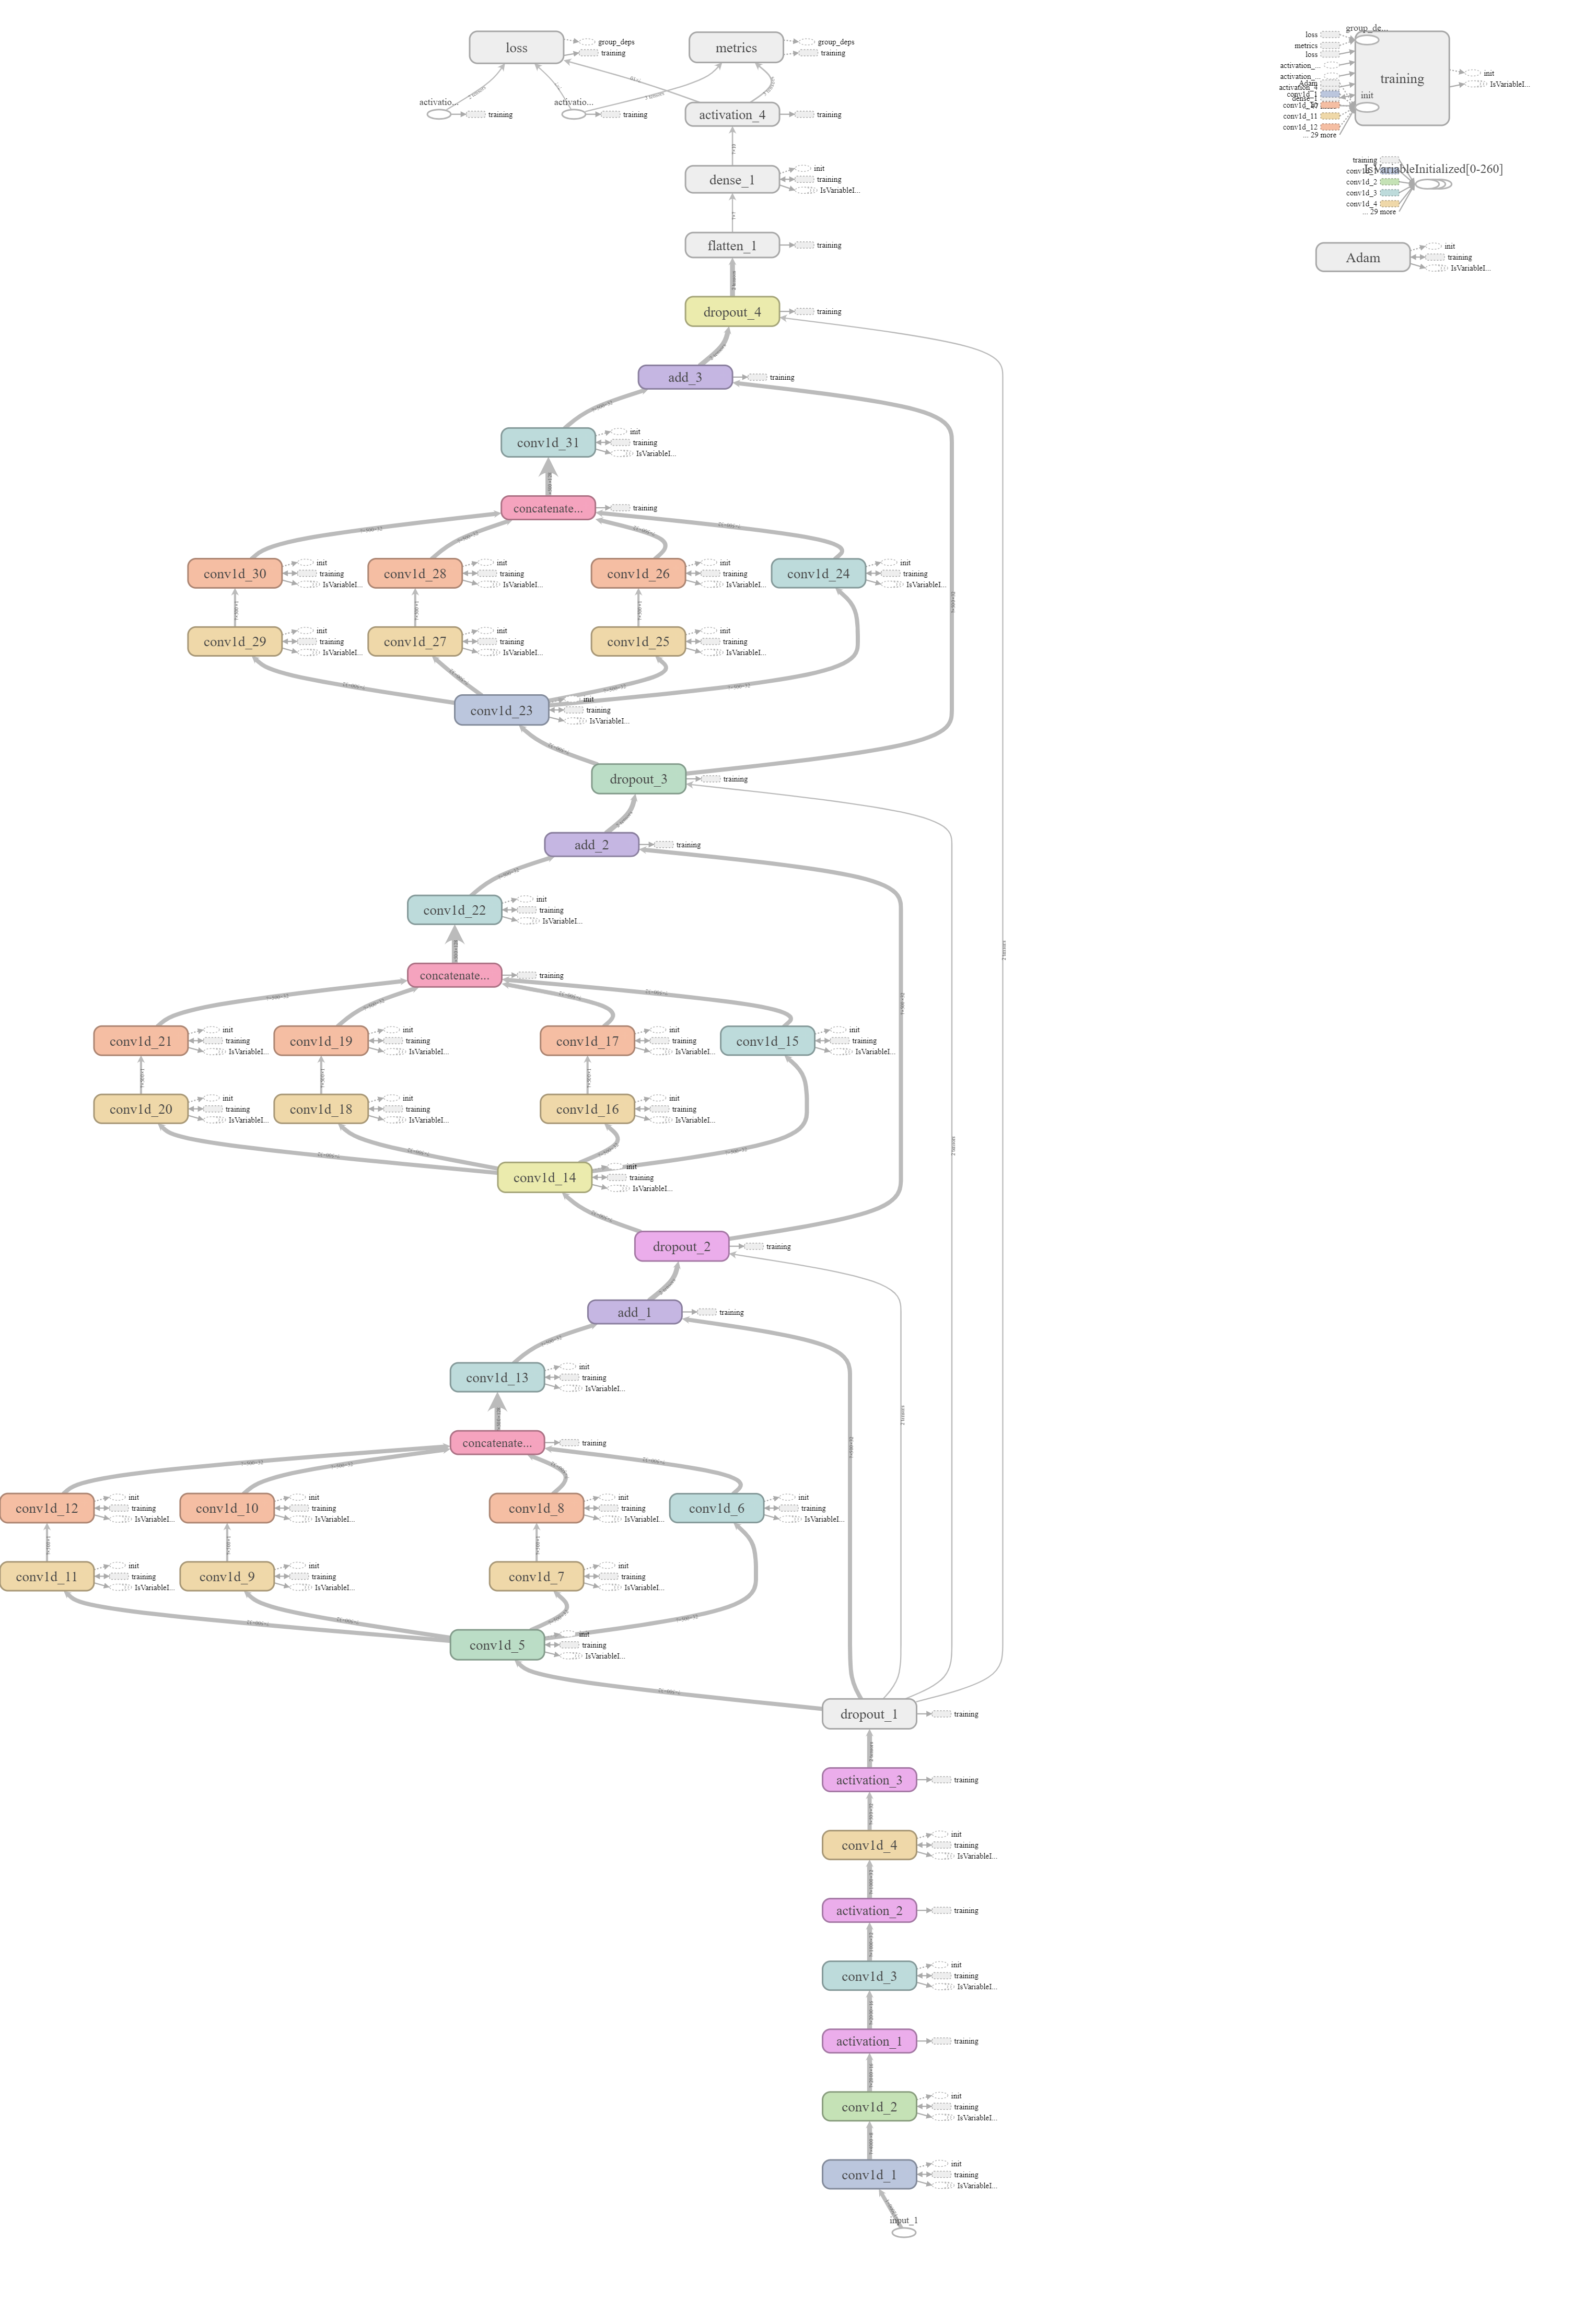
\includegraphics[height=0.85\textheight]{figures/modelA_diagram.png}
            \caption*{TensorBoard diagram of Model A.}
        \end{figure}
        
        \subsection{Model B}
        \label{app:modelB_diagram}
        \texttt{Referred to in section \ref{sec:design_modelB}}
        \begin{figure}[H]
            \centering
            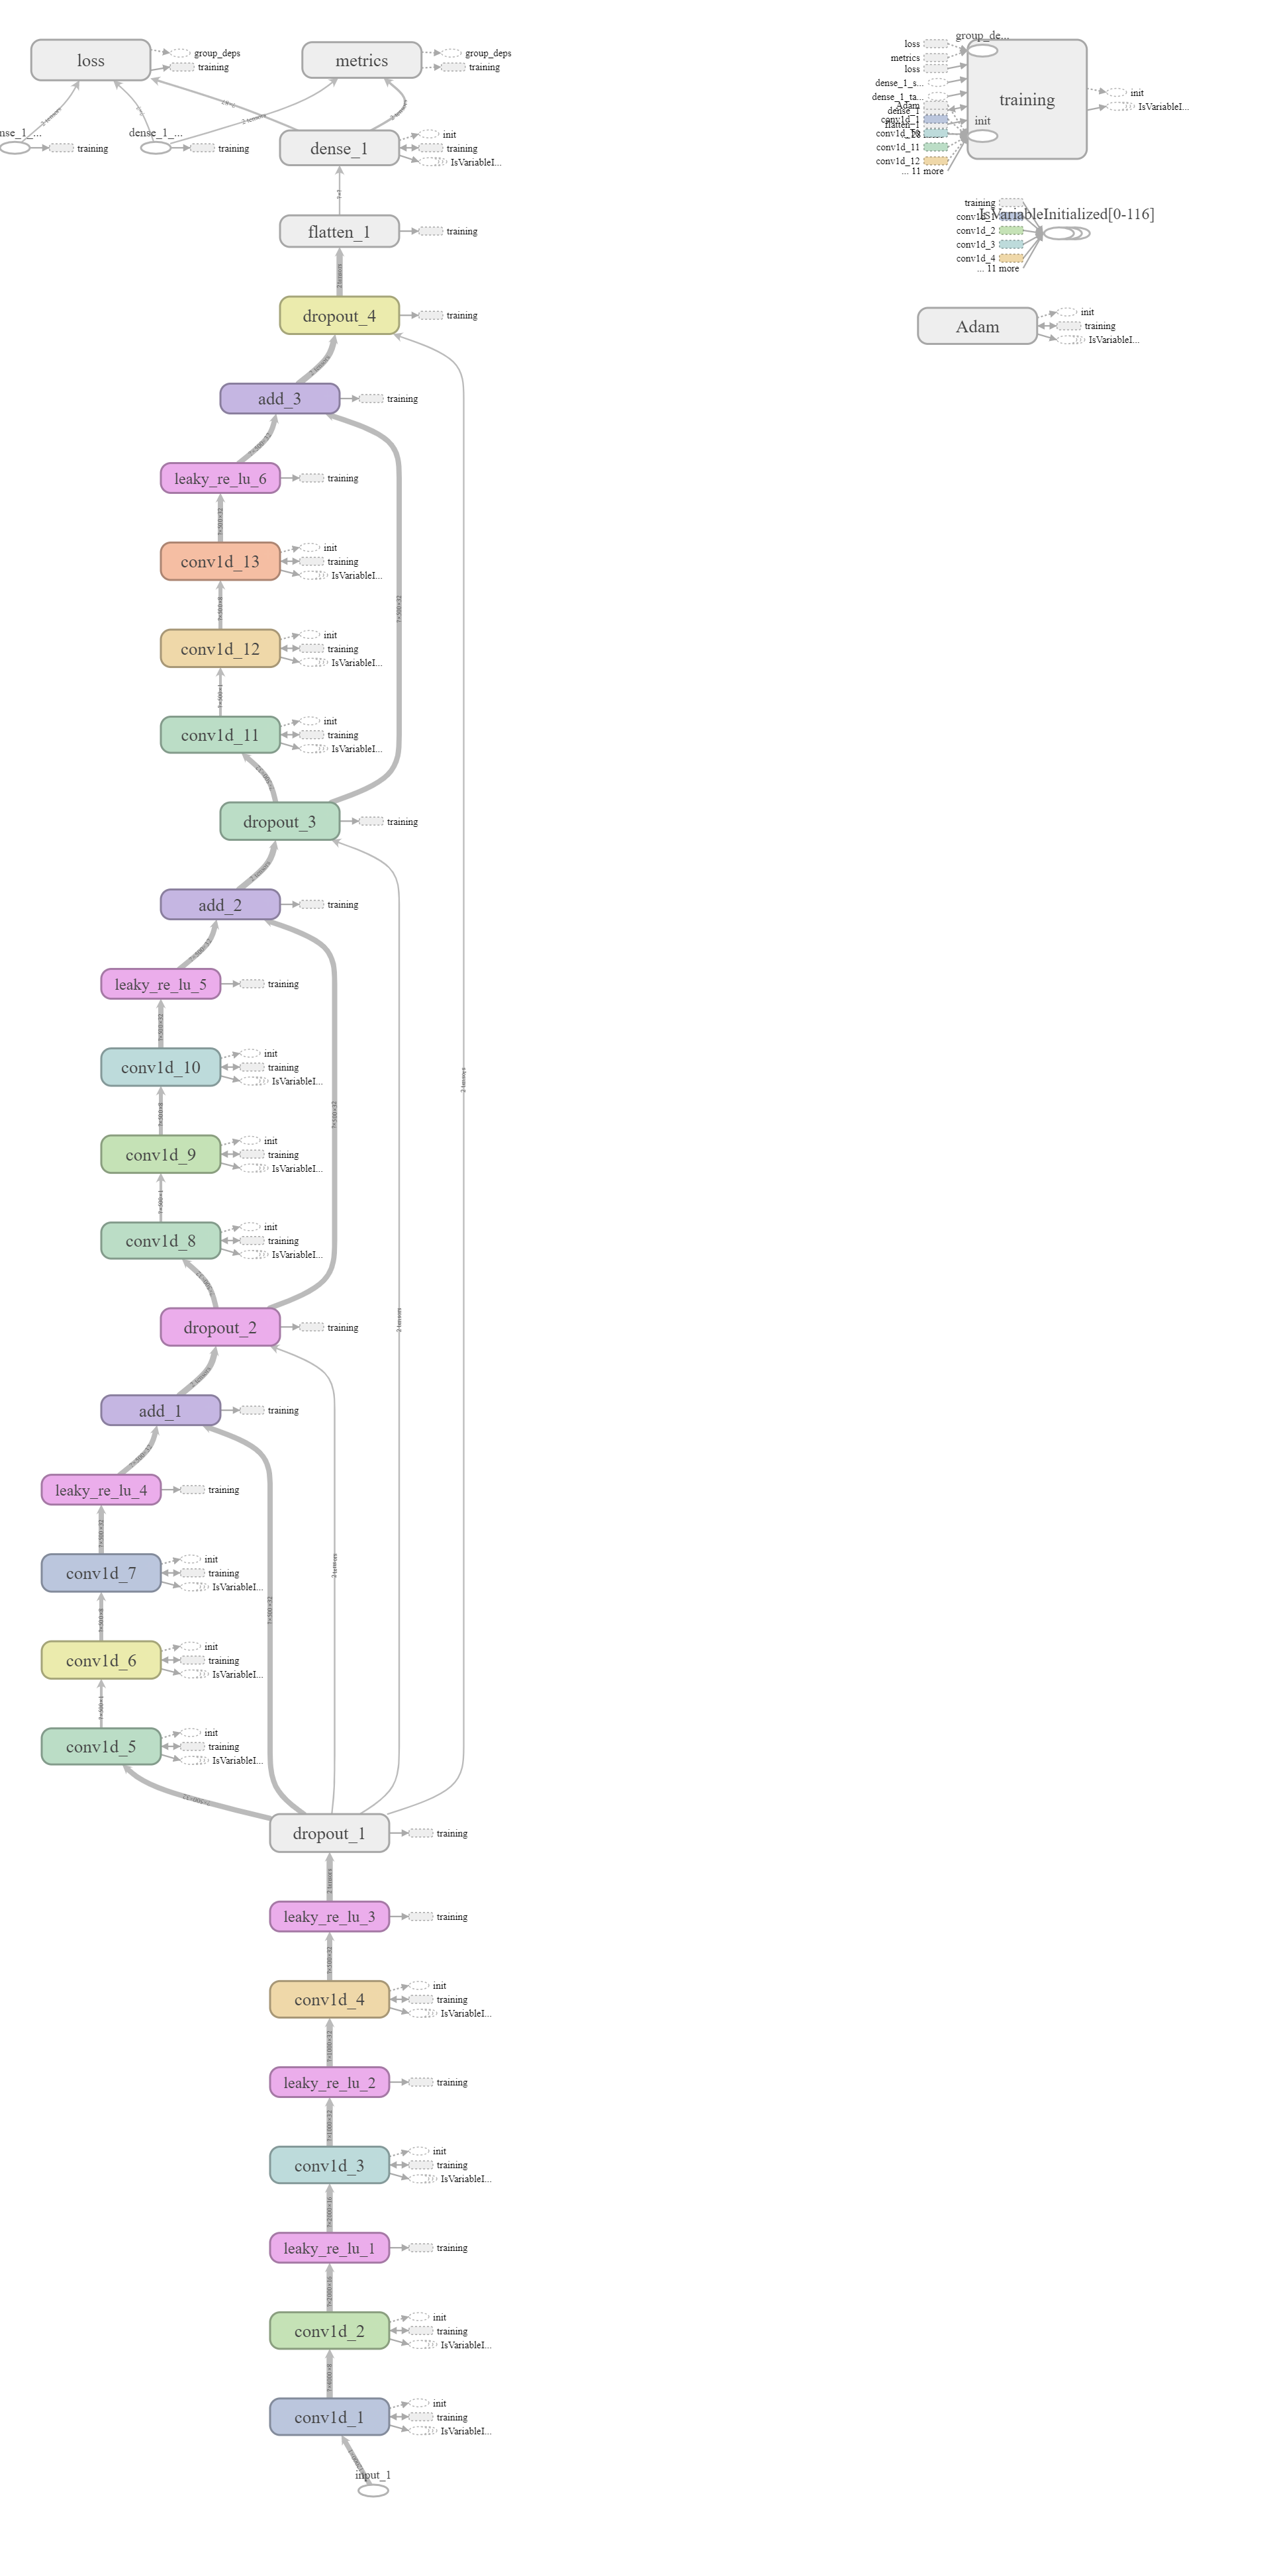
\includegraphics[height=0.85\textheight]{figures/modelB_diagram.png}
            \caption*{TensorBoard diagram of Model B.}
        \end{figure}
        
        \subsection{Model C}
        \label{app:modelC_diagram}
        \texttt{Referred to in section \ref{sec:design_modelC}}
        \begin{figure}[H]
            \centering
            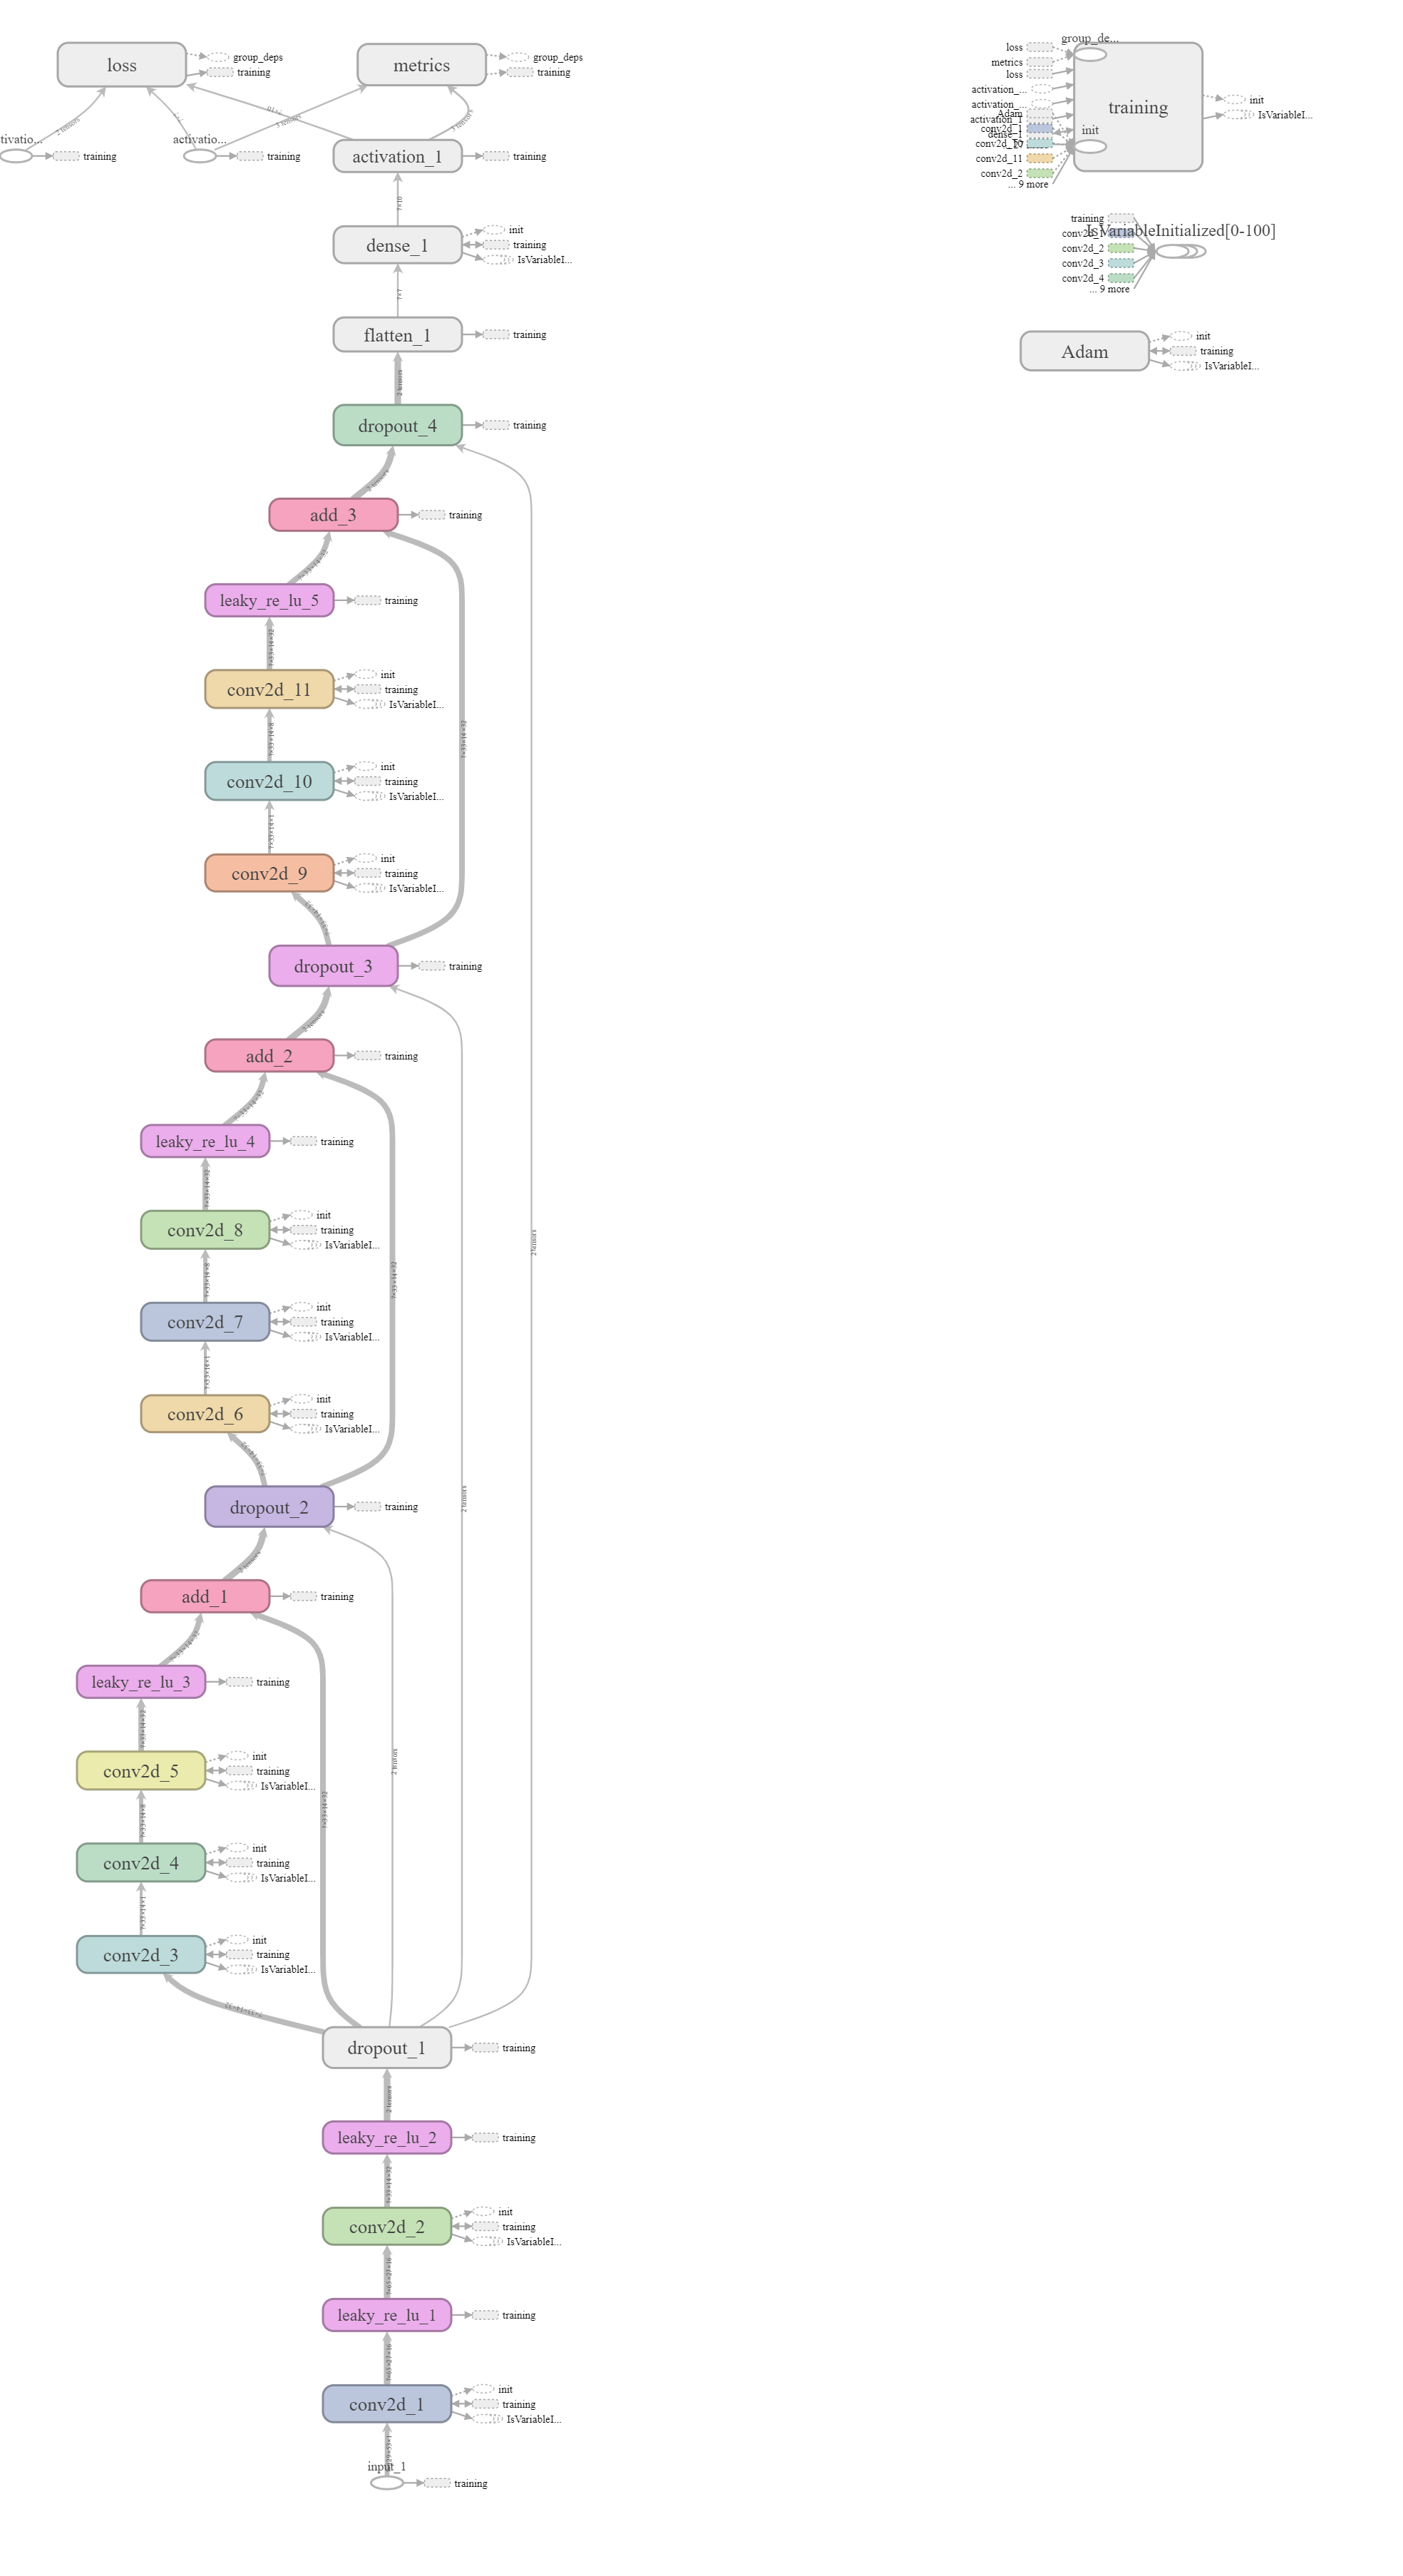
\includegraphics[height=0.85\textheight]{figures/modelC_diagram.png}
            \caption*{TensorBoard diagram of Model C.}
        \end{figure}
    
    \newpage
    \section{Training progress}
        \subsection{Optimisation algorithm comparison}
        \subsubsection{Loss during training}
        \label{app:optimisation_loss_during_training}
        \texttt{Referred to in section \ref{sec:training_analysis}}
        
        \begin{figure}[H]
            \centering
            \begin{tabular}{l|c|}
                Optimiser & Loss and validation loss during training\\
                \hline
                SGD & 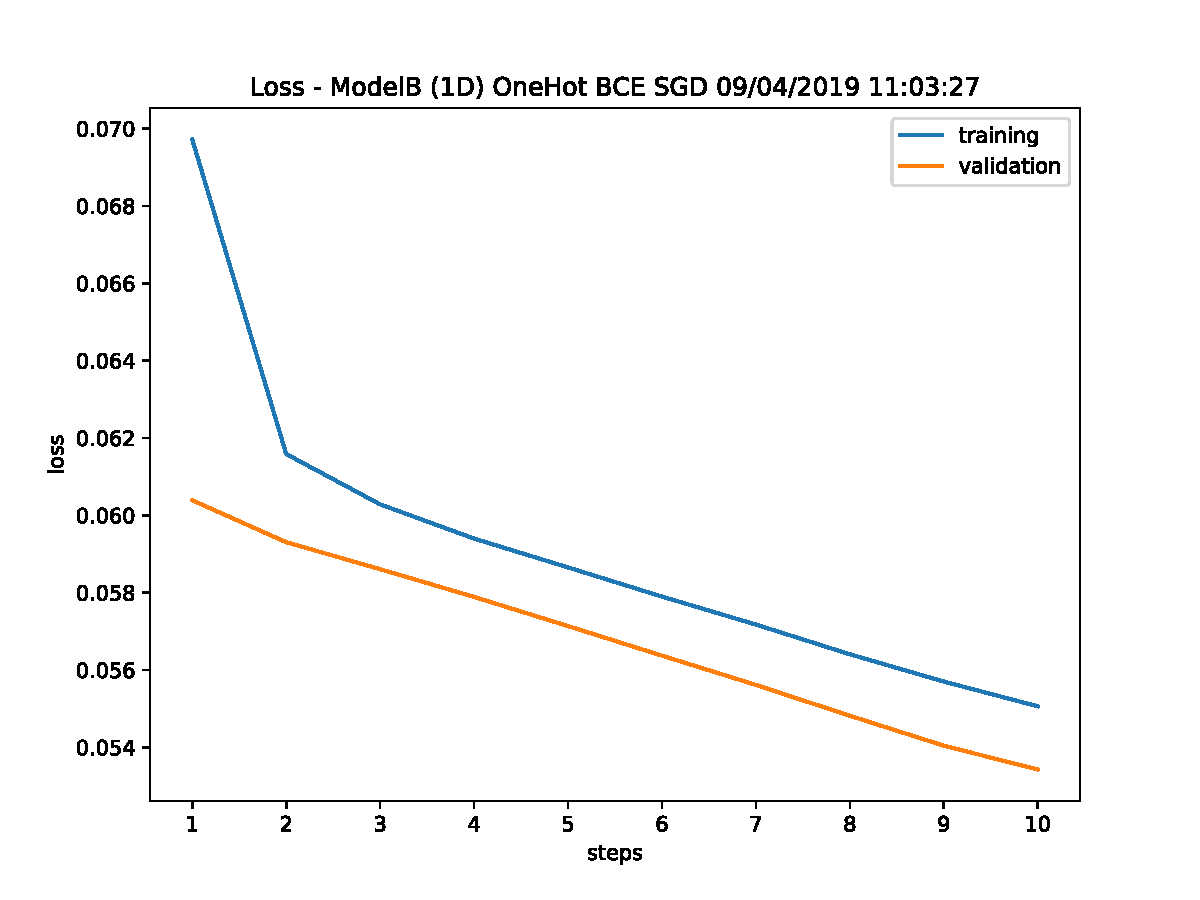
\includegraphics[width=0.7\textwidth,height=0.22\textheight,keepaspectratio]{figures/training_plots/ModelB-(1D)-OneHot-BCE-SGD_09-04-2019_11-03-27_loss.pdf}\\
                \hline
                ADAGRAD & 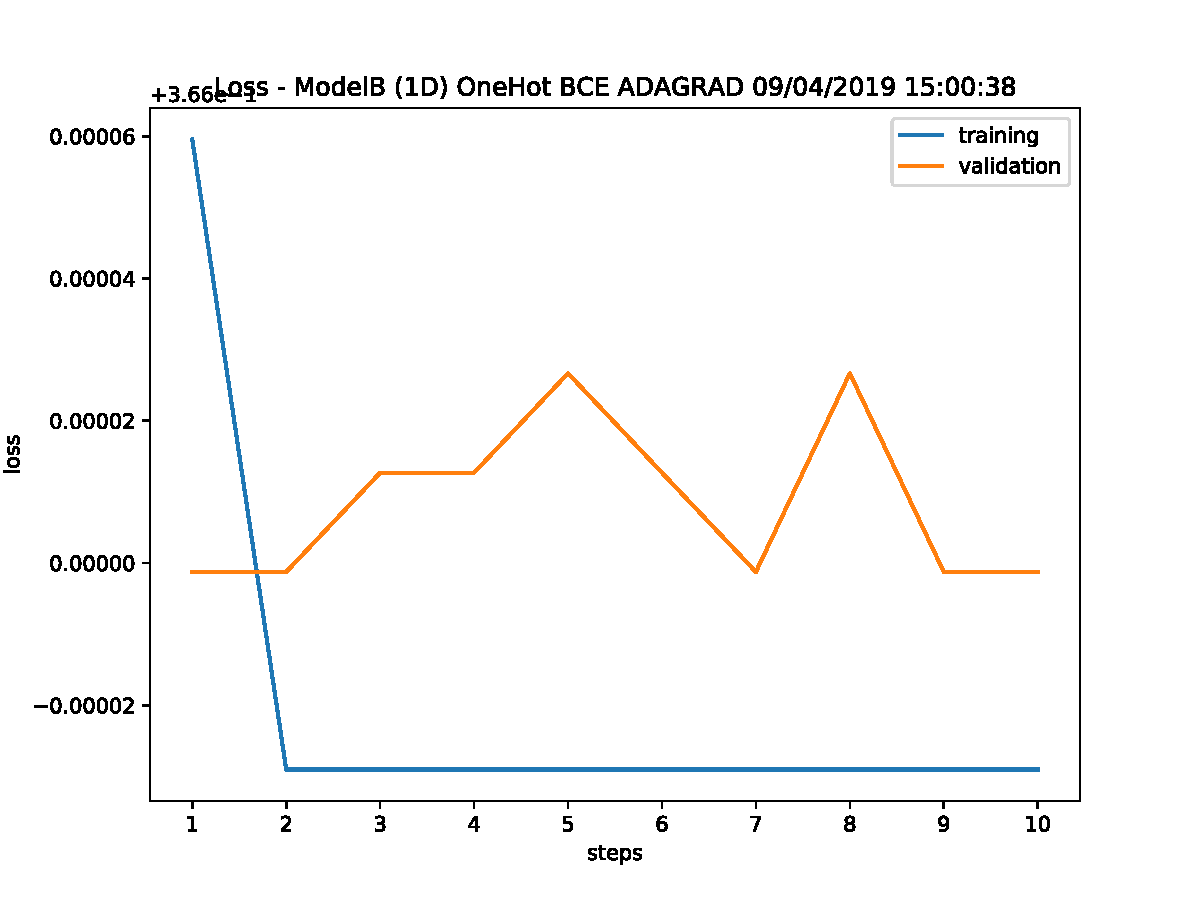
\includegraphics[width=0.7\textwidth,height=0.22\textheight,keepaspectratio]{figures/training_plots/ModelB-(1D)-OneHot-BCE-ADAGRAD_09-04-2019_15-00-38_loss.pdf}\\
                \hline
                ADAM & 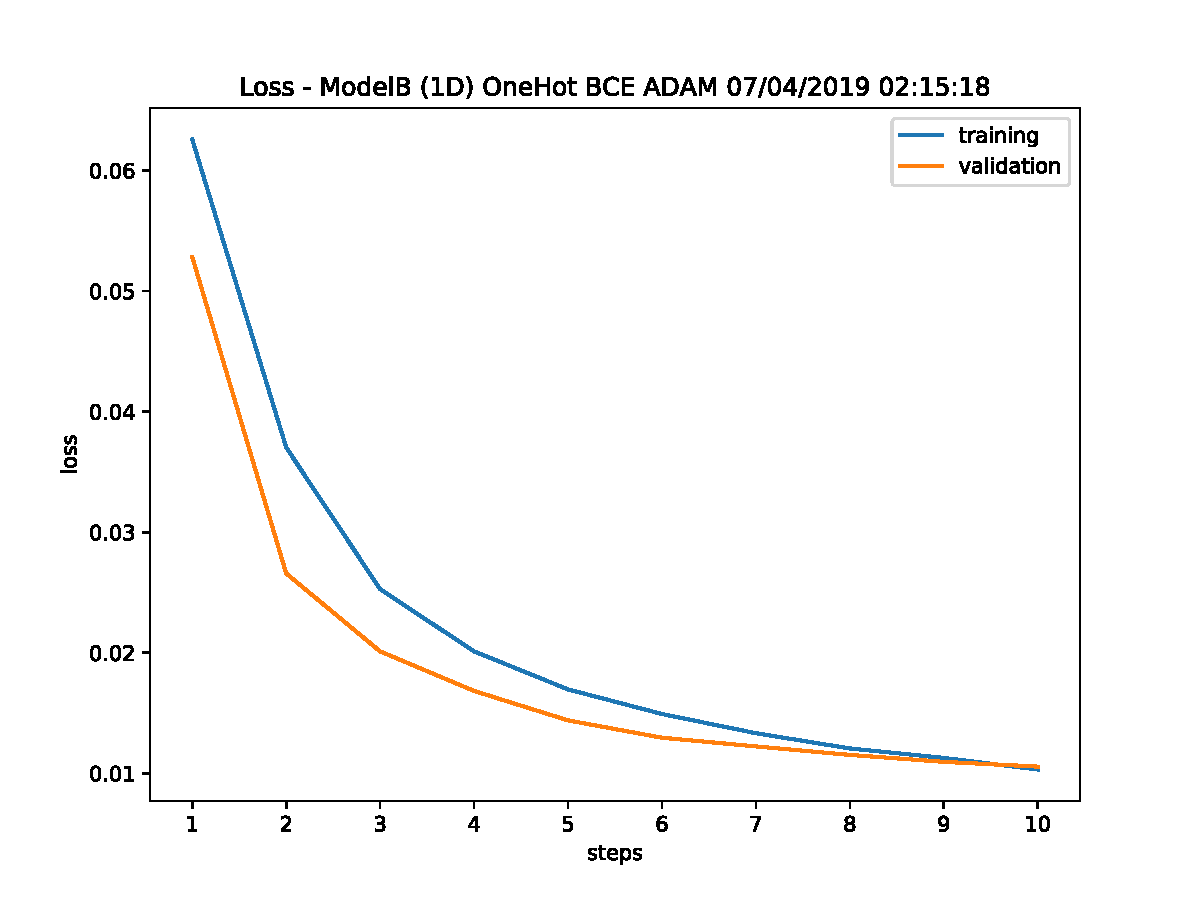
\includegraphics[width=0.7\textwidth,height=0.22\textheight,keepaspectratio]{figures/training_plots/ModelB-(1D)-OneHot-BCE-ADAM_07-04-2019_02-15-18_loss.pdf} 
            \end{tabular}
            \caption*{The loss values during training for Model B with one-hot encoding and BCE loss when using different optimiser algorithms. \textit{Note: the vertical scale of the middle figure (for ADAGRAD) is +0.366.}}
        \end{figure}
        
        \subsubsection{Training processing times}
        \label{app:optimisation_processing_times}
        \texttt{Referred to in section \ref{sec:training_analysis}}
        
        \begin{figure}[H]
            \centering
            \begin{tabular}{l|c|c|c|c|c|c|c|c|c|c|c|}
                \multirow{2}{*}{Optimiser} & \multicolumn{10}{c|}{Epoch} & \multirow{2}{*}{Total}\\
                    \cline{2-11}
                    & 1 & 2 & 3 & 4 & 5 & 6 & 7 & 8 & 9 & 10 &\\
                    \hline
                ADAGRAD & 24.0 & 23.0 & 23.1 & 25.1 & 21.4 & 24.3 & 26.9 & 22.3 & 22.2 & 24.8 & 237.0\\
                ADAM & 24.3 & 19.0 & 19.0 & 19.0 & 19.1 & 19.0 & 18.9 & 19.1 & 19.0 & 18.9 & 195.3\\
                SGD & 23.6 & 22.3 & 22.7 & 28.4 & 21.8 & 24.2 & 19.3 & 18.9 & 19.0 & 18.9 & 219.0
            \end{tabular}
            \caption*{The duration of each epoch as well as total time taken for 10 epochs in minutes. For different optimisation algorithms on Model B with one-hot encoding and BCE loss.}
        \end{figure}
        
        \subsection{All model processing times with ADAM optimiser}
        \label{app:model_processing_times}
        \texttt{Referred to in section \ref{sec:training_analysis}}
        
        \begin{figure}[H]
            \centering
            \begin{footnotesize}
                \begin{tabular}{l|c|c|c|c|c|c|c|c|c|c|c|}
                    \multirow{2}{*}{Model and configuration} & \multicolumn{10}{c|}{Epoch} & \multirow{2}{*}{Total}\\
                    \cline{2-11}
                    & 1 & 2 & 3 & 4 & 5 & 6 & 7 & 8 & 9 & 10 &\\
                    \hline
                    ModelA (1D) MultiHot BCE & 24.8 & 19.6 & 19.1 & 19.3 & 19.2 & 19.2 & 19.3 & 19.4 & 19.1 & 19.2 & 198.1\\
                    ModelA (1D) MultiHot KLD & 25.7 & 20.2 & 19.5 & 19.4 & 19.3 & 21.8 & 22.7 & 25.9 & 19.2 & 19.2 & 212.8\\
                    ModelA (1D) OneHot BCE & 35.6 & 44.4 & 42.7 & 46.6 & 43.1 & 43.3 & 42.2 & 42.5 & 42.2 & 43.5 & 426.0\\
                    ModelA (1D) OneHot KLD & 24.0 & 24.5 & 26.5 & 34.6 & 20.2 & 19.4 & 19.5 & 19.3 & 19.5 & 19.5 & 227.0\\
                    ModelB (1D) MultiHot BCE & 24.3 & 27.3 & 22.2 & 19.0 & 18.7 & 18.7 & 19.0 & 19.1 & 18.8 & 18.9 & 205.9\\
                    ModelB (1D) MultiHot KLD & 25.8 & 22.6 & 20.2 & 20.7 & 20.2 & 20.2 & 20.4 & 20.2 & 20.1 & 20.2 & 210.6\\
                    ModelB (1D) OneHot BCE & 24.3 & 19.0 & 19.0 & 19.0 & 19.1 & 19.0 & 18.9 & 19.1 & 19.0 & 18.9 & 195.3\\
                    ModelB (1D) OneHot KLD & 24.7 & 19.2 & 18.8 & 19.0 & 19.0 & 18.9 & 19.0 & 19.1 & 19.3 & 19.3 & 196.4\\
                    ModelC (lin 2D) MultiHot BCE & 24.3 & 18.8 & 19.0 & 19.0 & 19.0 & 19.1 & 19.0 & 19.0 & 19.3 & 23.9 & 200.3\\
                    ModelC (lin 2D) MultiHot KLD & 24.8 & 24.1 & 29.4 & 32.5 & 22.7 & 19.2 & 19.1 & 19.0 & 19.0 & 19.2 & 229.0\\
                    ModelC (lin 2D) OneHot BCE & 24.2 & 19.0 & 19.0 & 19.0 & 19.0 & 18.9 & 18.9 & 19.3 & 19.0 & 18.9 & 195.1\\
                    ModelC (lin 2D) OneHot KLD & 23.4 & 18.8 & 19.0 & 19.1 & 23.6 & 24.7 & 24.9 & 25.5 & 22.6 & 25.4 & 227.0\\
                    ModelC (log 2D) MultiHot BCE & 24.6 & 19.0 & 19.1 & 19.3 & 19.2 & 18.9 & 19.0 & 19.1 & 19.0 & 19.0 & 196.2\\
                    ModelC (log 2D) MultiHot KLD & 24.3 & 18.9 & 18.9 & 31.3 & 21.4 & 19.0 & 26.8 & 19.5 & 19.2 & 19.2 & 218.4\\
                    ModelC (log 2D) OneHot BCE & 23.0 & 23.3 & 25.6 & 23.9 & 19.4 & 20.0 & 19.5 & 20.0 & 19.3 & 20.2 & 214.2\\
                    ModelC (log 2D) OneHot KLD & 24.5 & 26.4 & 28.2 & 33.8 & 22.8 & 27.8 & 30.0 & 20.7 & 38.0 & 26.7 & 278.7
                \end{tabular}
            \end{footnotesize}
            \caption*{The duration of each epoch as well as total time taken for 10 epochs in minutes. For different models using ADAM optimisation.}
        \end{figure}
        
        \newpage
        \subsection{Model A training metrics}
        \label{app:modelA_training}
        \texttt{Referred to in section \ref{sec:training_analysis_modelA}}
        
        \begin{figure}[H]
            \centering
            \begin{tabular}{cc}
                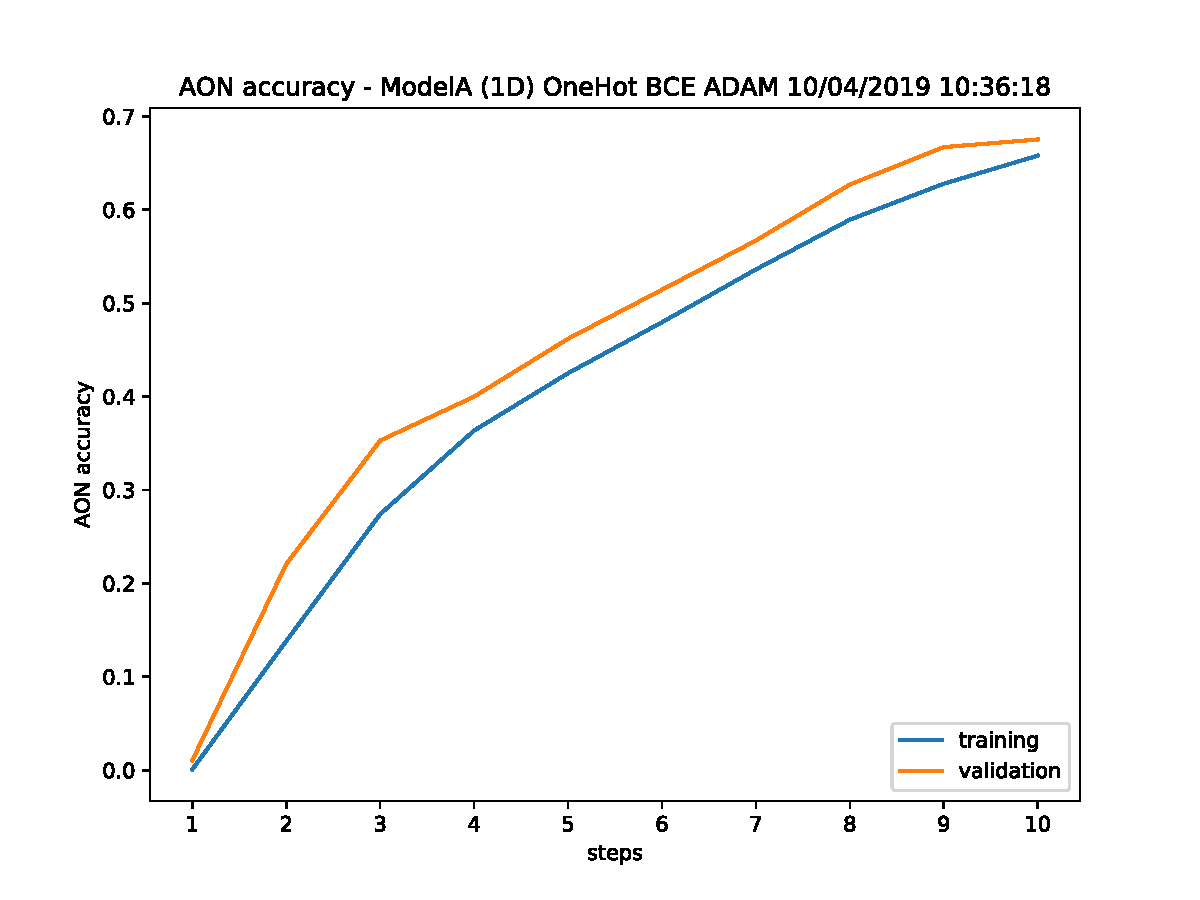
\includegraphics[width=0.45\textwidth]{figures/training_plots/ModelA-(1D)-OneHot-BCE-ADAM_10-04-2019_10-36-18_AON-accuracy.pdf} & 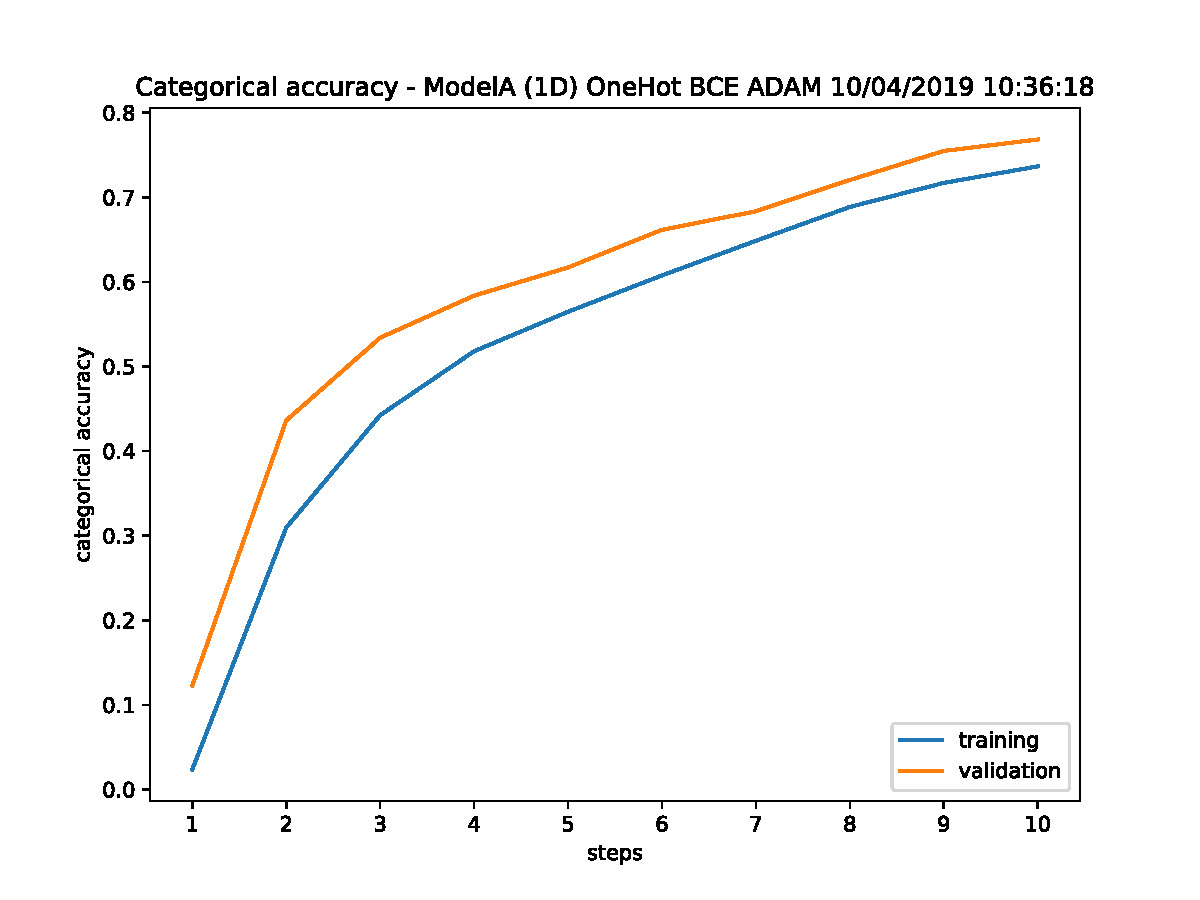
\includegraphics[width=0.45\textwidth]{figures/training_plots/ModelA-(1D)-OneHot-BCE-ADAM_10-04-2019_10-36-18_categorical-accuracy.pdf} \\
                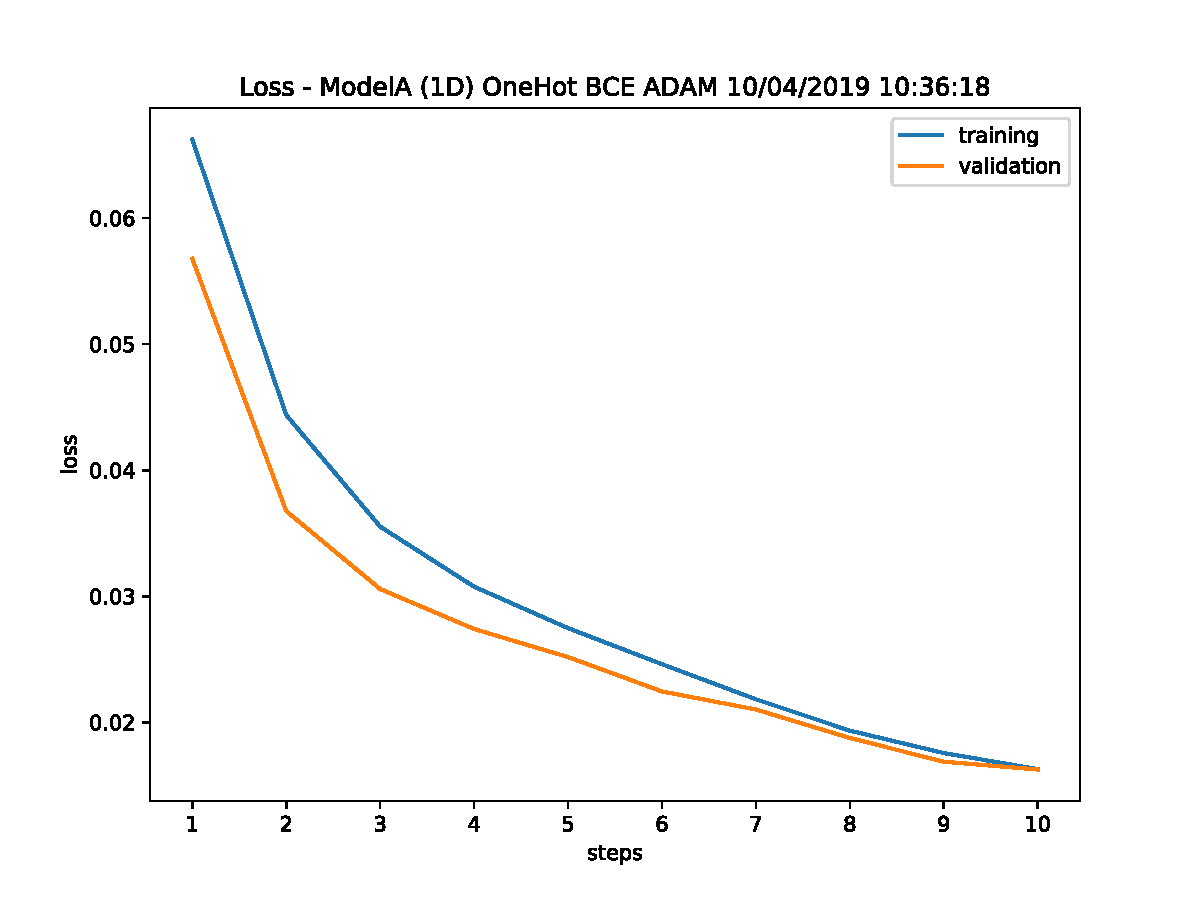
\includegraphics[width=0.45\textwidth]{figures/training_plots/ModelA-(1D)-OneHot-BCE-ADAM_10-04-2019_10-36-18_loss.pdf} & 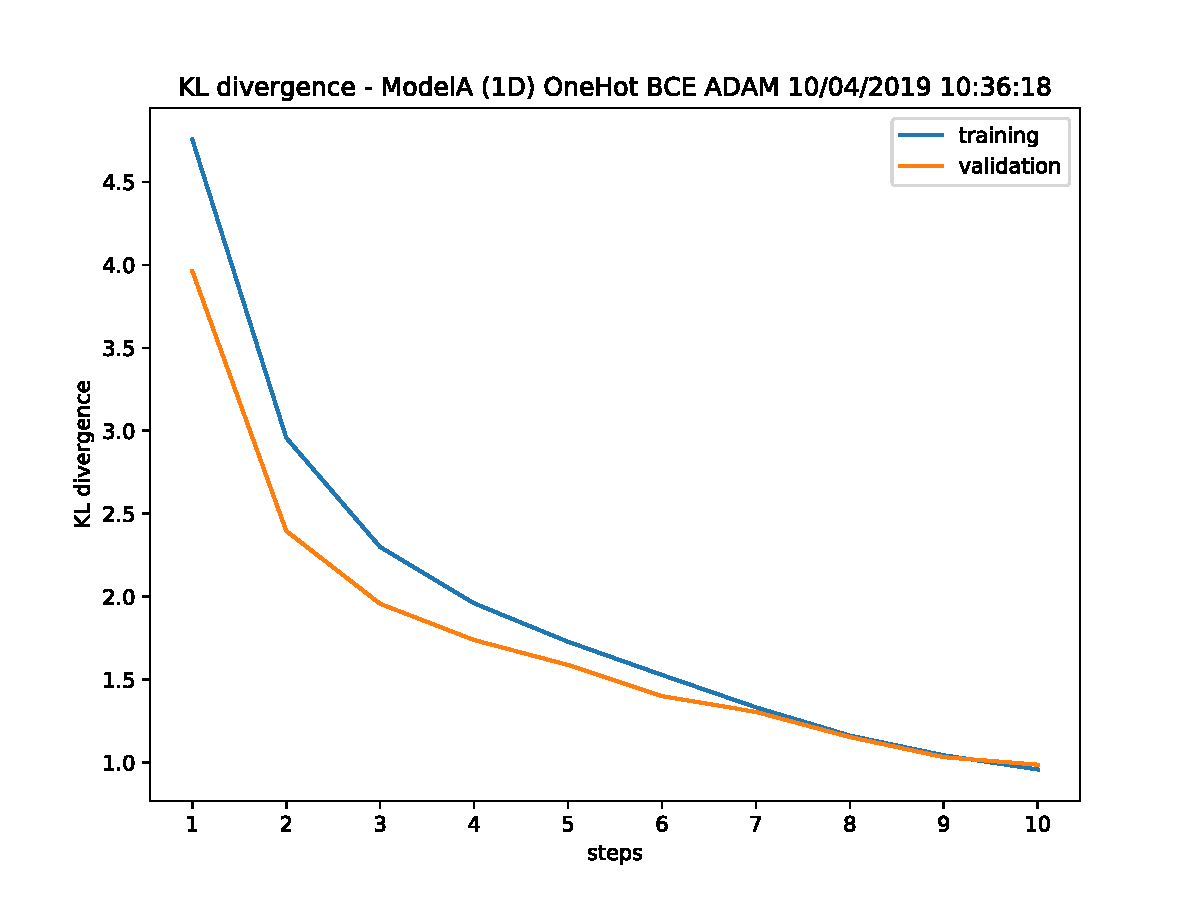
\includegraphics[width=0.45\textwidth]{figures/training_plots/ModelA-(1D)-OneHot-BCE-ADAM_10-04-2019_10-36-18_KL-divergence.pdf}
            \end{tabular}
            \caption*{One-hot encoding, BCE loss}
        \end{figure}
        
        \begin{figure}[H]
            \centering
            \begin{tabular}{cc}
                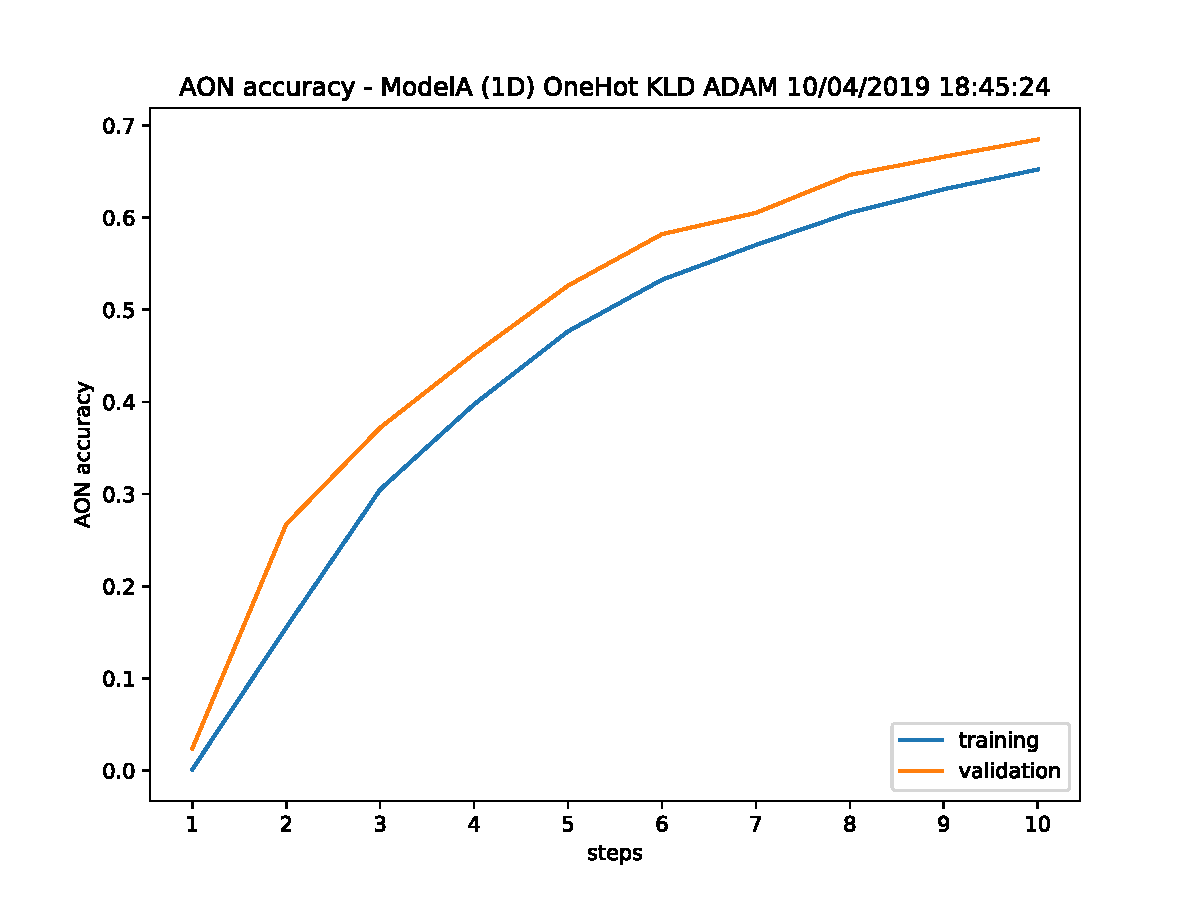
\includegraphics[width=0.45\textwidth]{figures/training_plots/ModelA-(1D)-OneHot-KLD-ADAM_10-04-2019_18-45-24_AON-accuracy.pdf} & 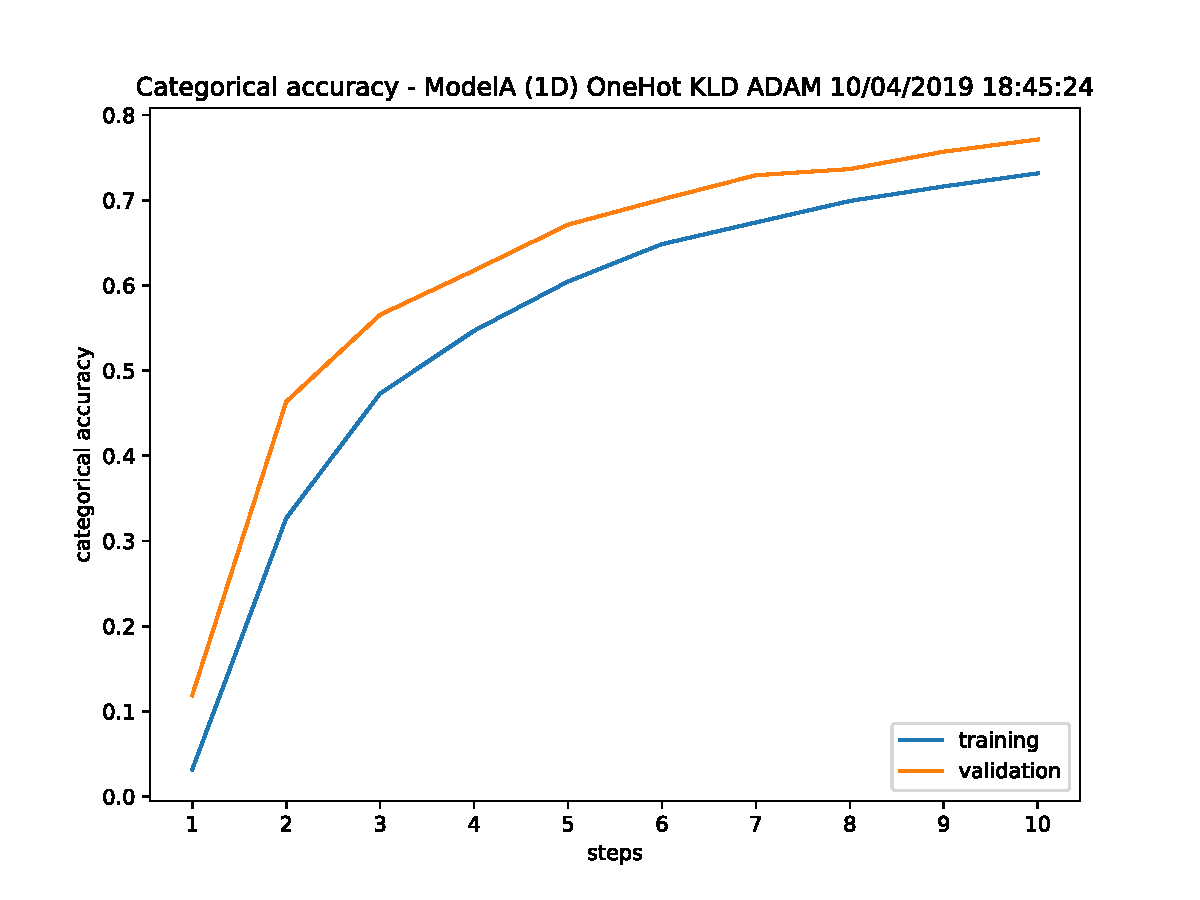
\includegraphics[width=0.45\textwidth]{figures/training_plots/ModelA-(1D)-OneHot-KLD-ADAM_10-04-2019_18-45-24_categorical-accuracy.pdf} \\
                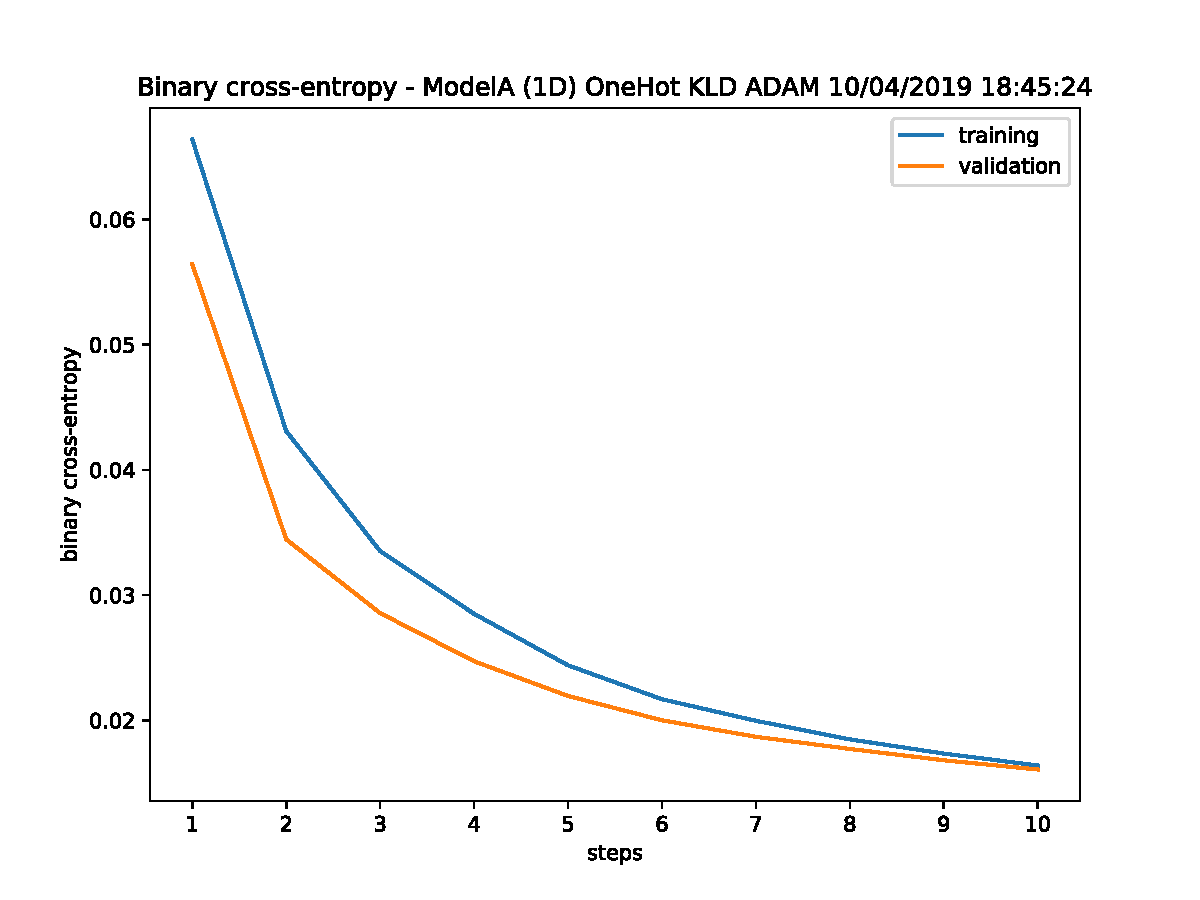
\includegraphics[width=0.45\textwidth]{figures/training_plots/ModelA-(1D)-OneHot-KLD-ADAM_10-04-2019_18-45-24_binary-cross-entropy.pdf} & 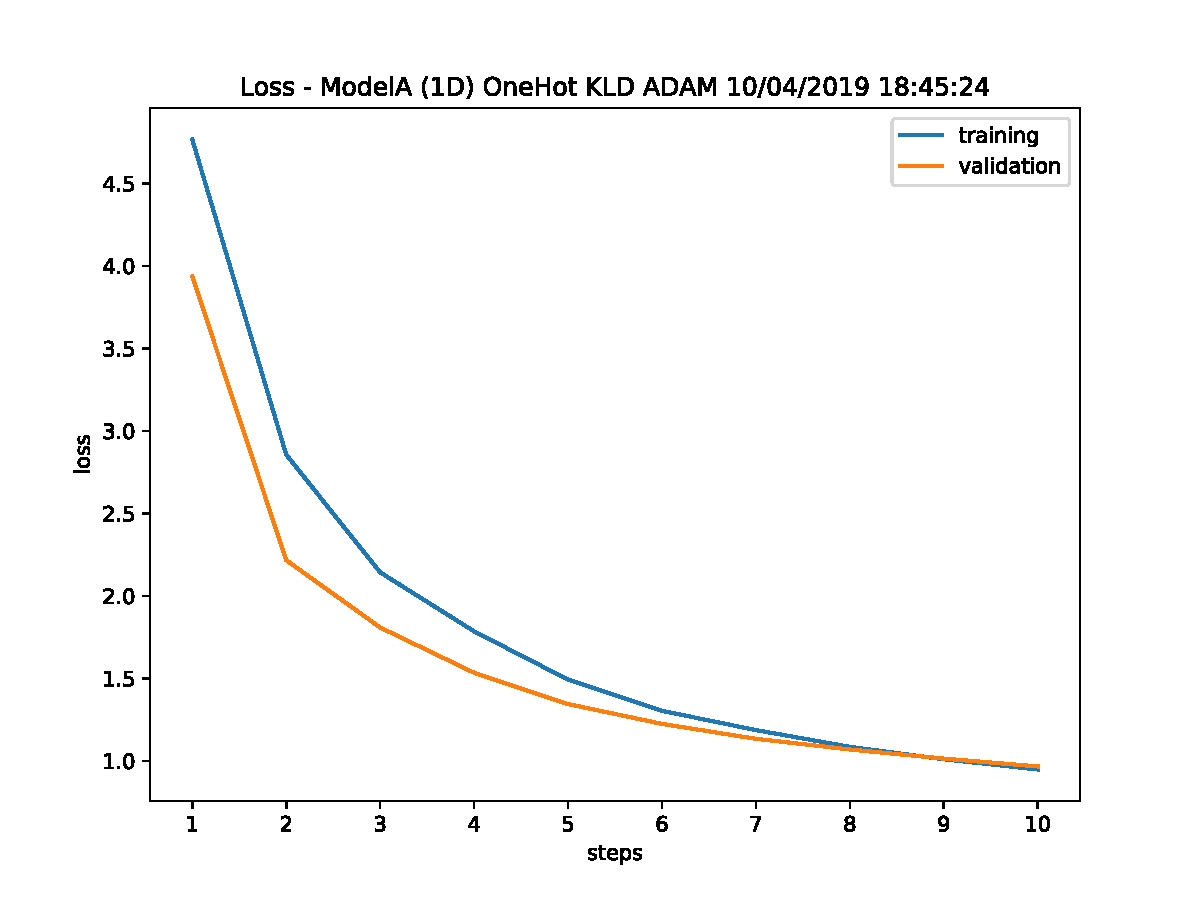
\includegraphics[width=0.45\textwidth]{figures/training_plots/ModelA-(1D)-OneHot-KLD-ADAM_10-04-2019_18-45-24_loss.pdf}
            \end{tabular}
            \caption*{One-hot encoding, KLD loss}
        \end{figure}
        
        \begin{figure}[H]
            \centering
            \begin{tabular}{cc}
                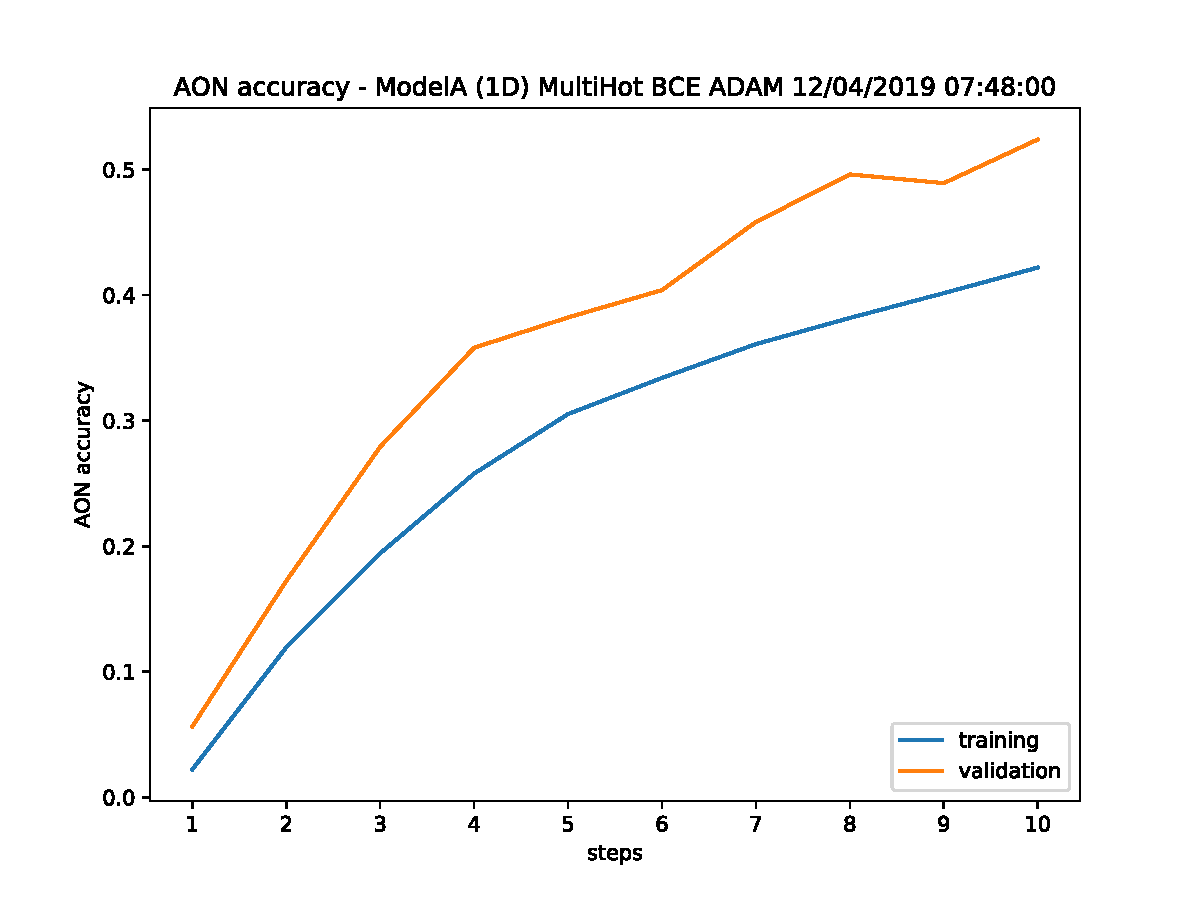
\includegraphics[width=0.48\textwidth]{figures/training_plots/ModelA-(1D)-MultiHot-BCE-ADAM_12-04-2019_07-48-00_AON-accuracy.pdf} & 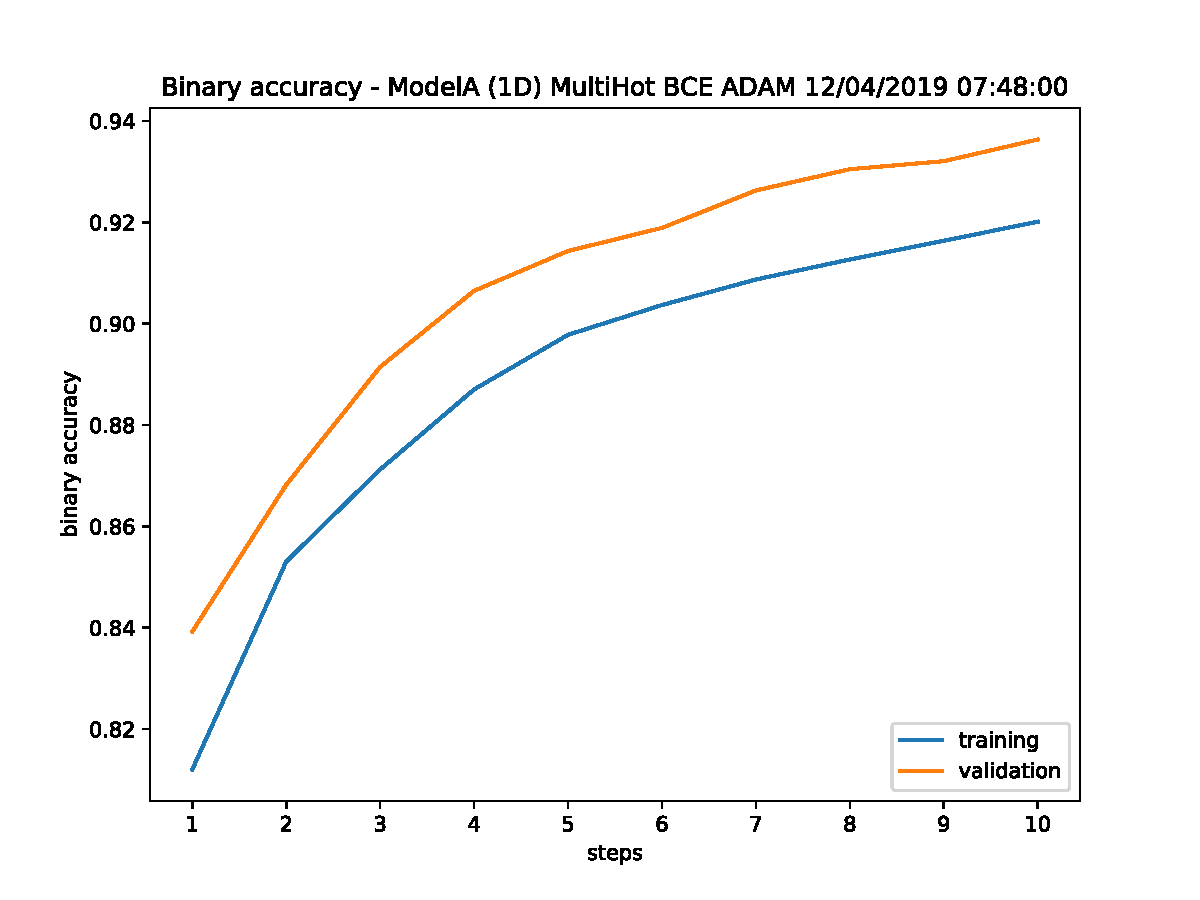
\includegraphics[width=0.48\textwidth]{figures/training_plots/ModelA-(1D)-MultiHot-BCE-ADAM_12-04-2019_07-48-00_binary-accuracy.pdf} \\
                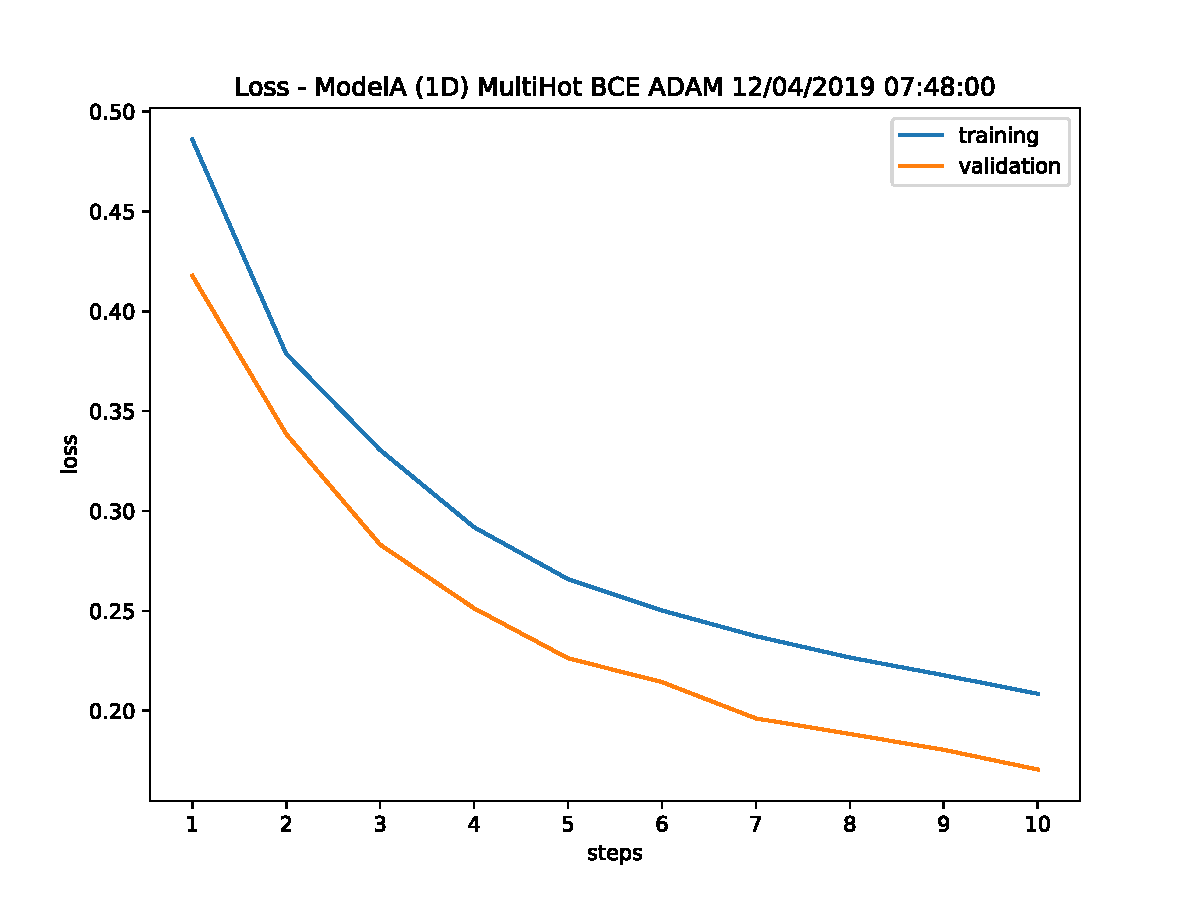
\includegraphics[width=0.48\textwidth]{figures/training_plots/ModelA-(1D)-MultiHot-BCE-ADAM_12-04-2019_07-48-00_loss.pdf} & 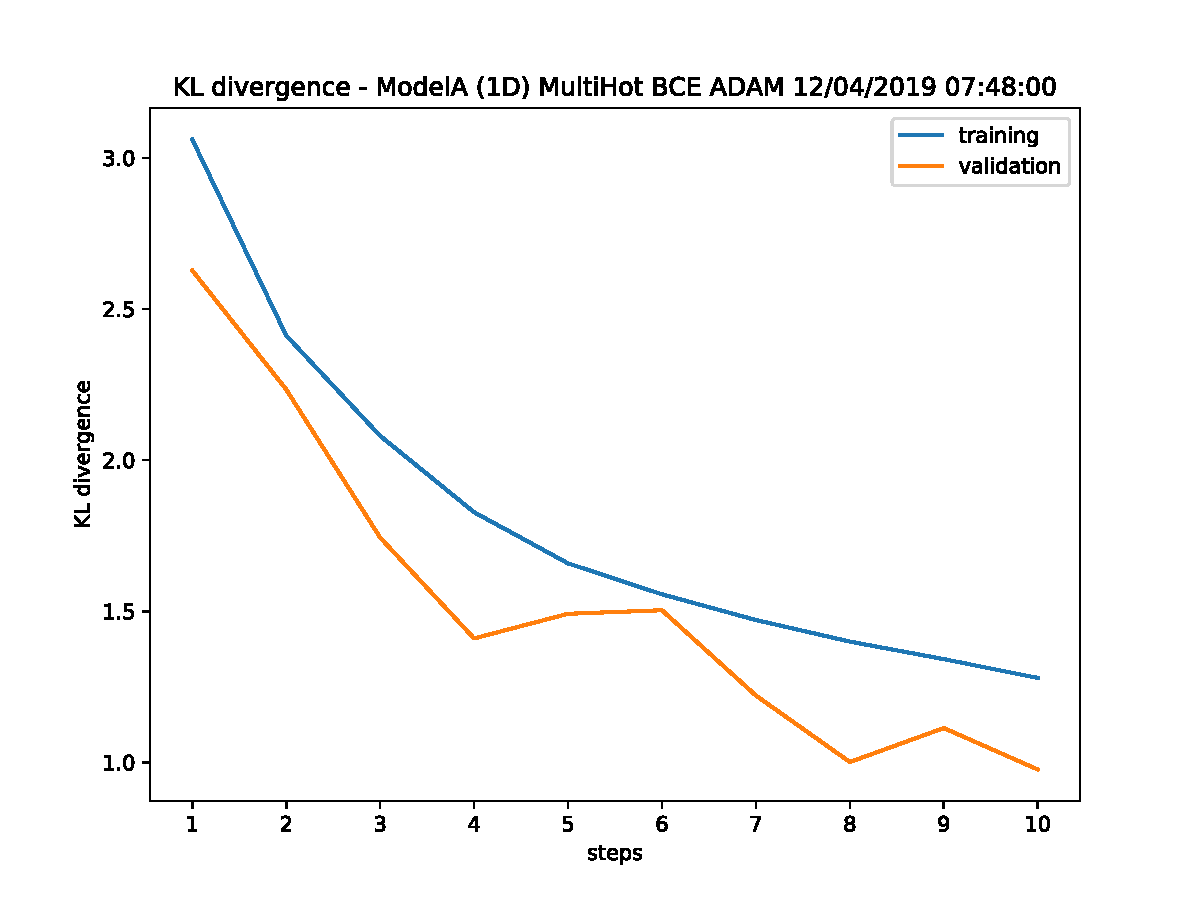
\includegraphics[width=0.48\textwidth]{figures/training_plots/ModelA-(1D)-MultiHot-BCE-ADAM_12-04-2019_07-48-00_KL-divergence.pdf}
            \end{tabular}
            \caption*{Multi-hot encoding, BCE loss}
        \end{figure}
        
        \begin{figure}[H]
            \centering
            \begin{tabular}{cc}
                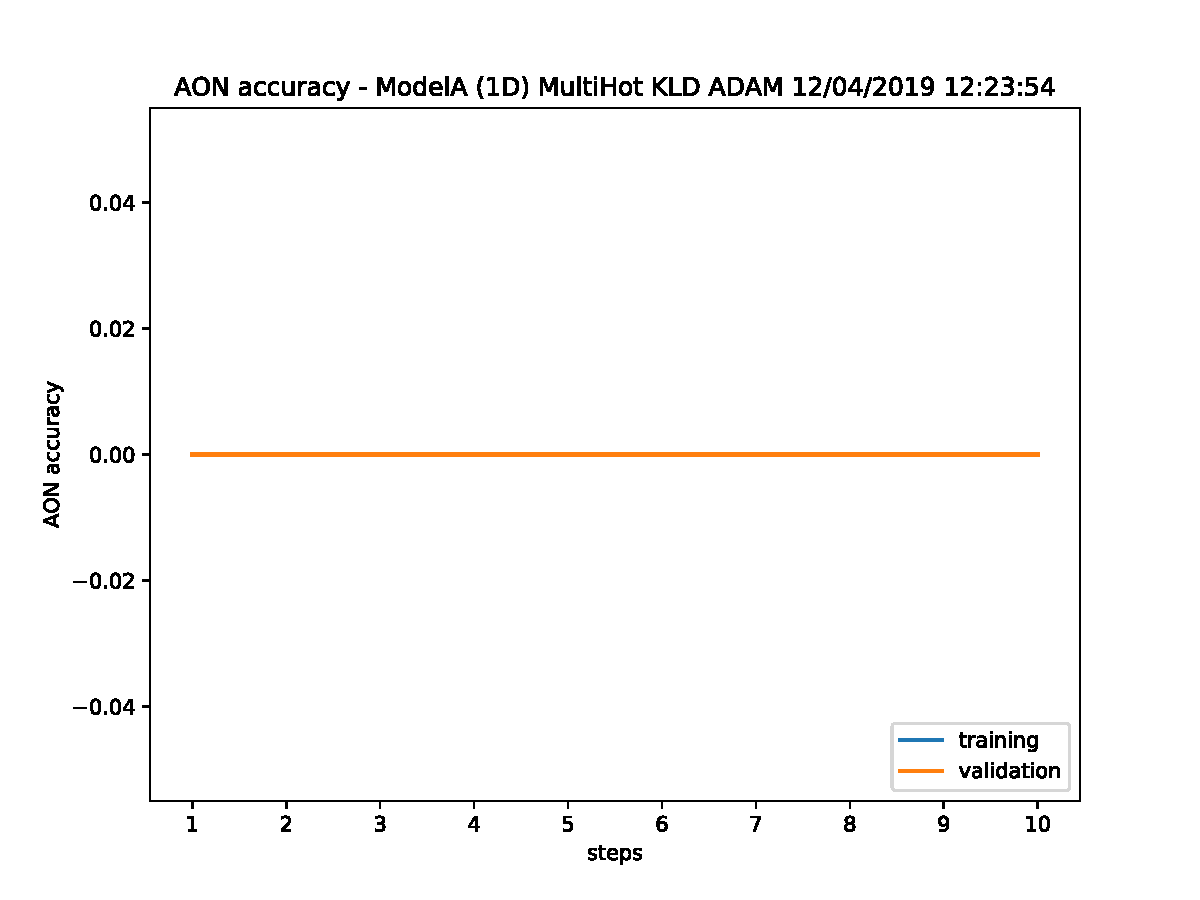
\includegraphics[width=0.48\textwidth]{figures/training_plots/ModelA-(1D)-MultiHot-KLD-ADAM_12-04-2019_12-23-54_AON-accuracy.pdf} & 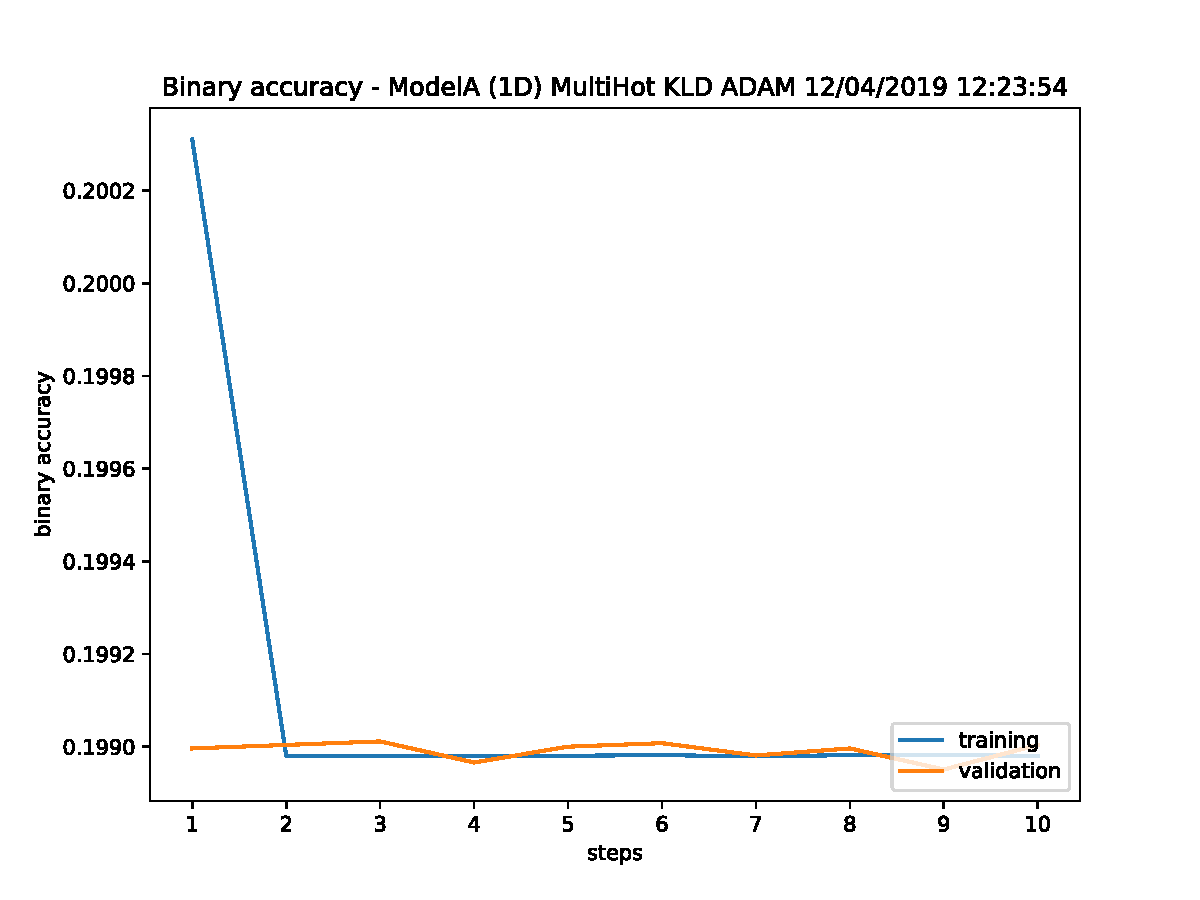
\includegraphics[width=0.48\textwidth]{figures/training_plots/ModelA-(1D)-MultiHot-KLD-ADAM_12-04-2019_12-23-54_binary-accuracy.pdf} \\
                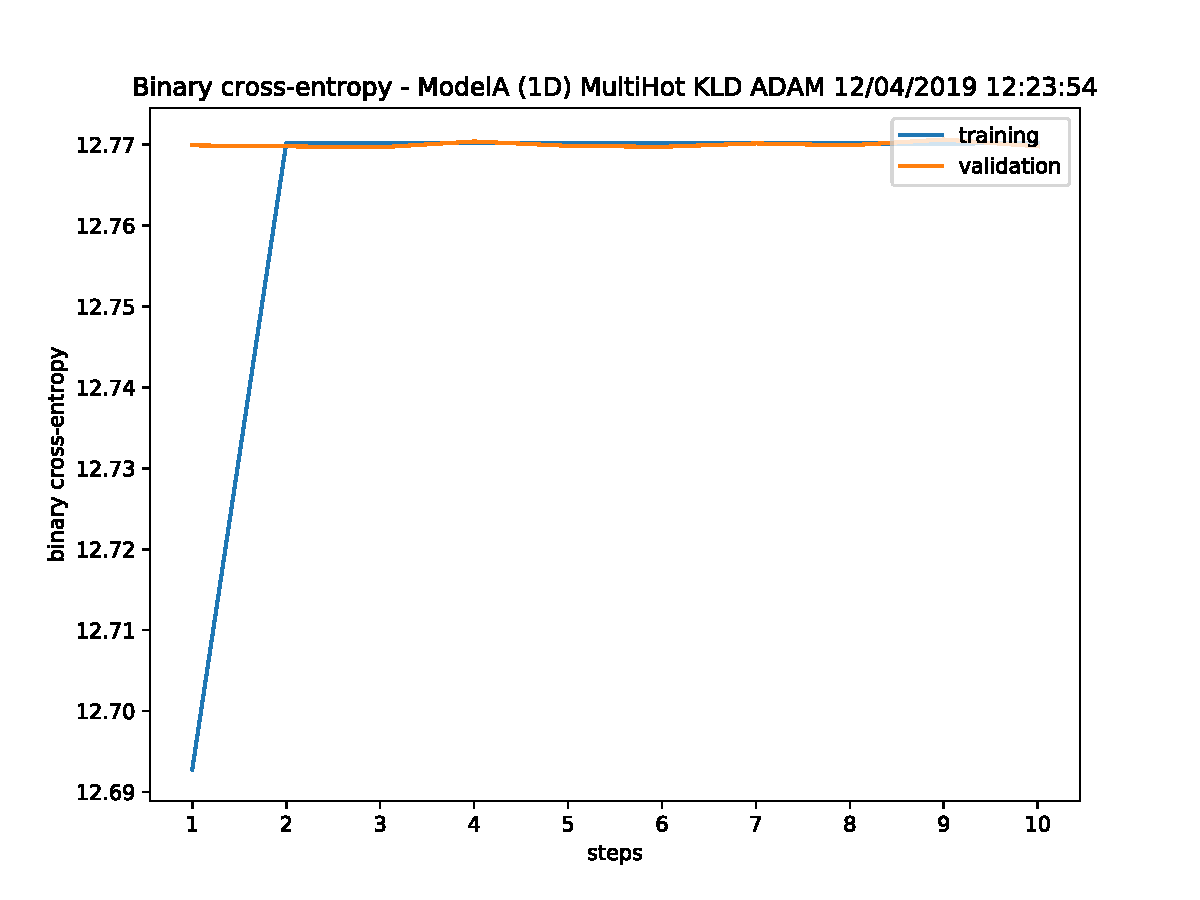
\includegraphics[width=0.48\textwidth]{figures/training_plots/ModelA-(1D)-MultiHot-KLD-ADAM_12-04-2019_12-23-54_binary-cross-entropy.pdf} & 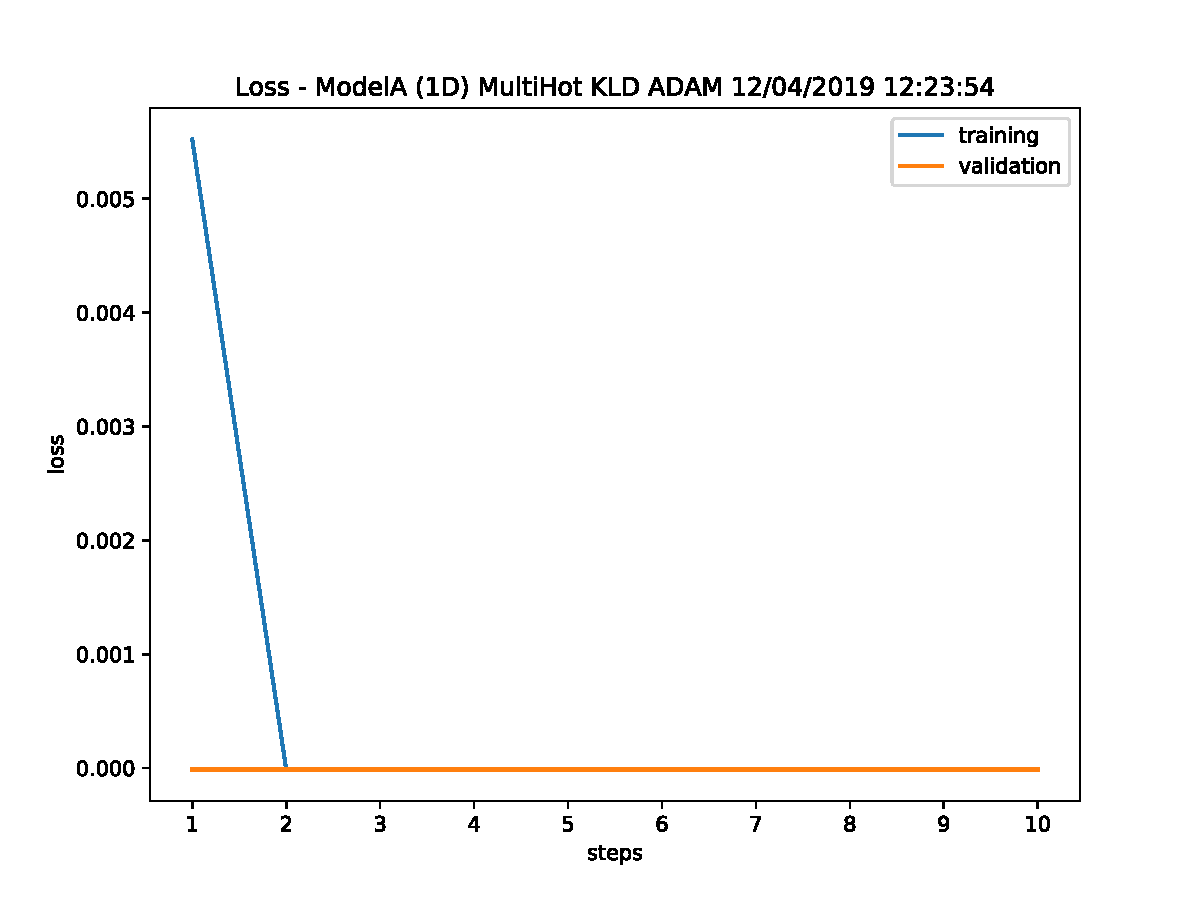
\includegraphics[width=0.48\textwidth]{figures/training_plots/ModelA-(1D)-MultiHot-KLD-ADAM_12-04-2019_12-23-54_loss.pdf}
            \end{tabular}
            \caption*{Multi-hot encoding, KLD loss}
        \end{figure}
        
        \subsection{Model B training metrics}
        \label{app:modelB_training}
        \texttt{Referred to in section \ref{sec:training_analysis_modelB}}
        
        \begin{figure}[H]
            \centering
            \begin{tabular}{cc}
                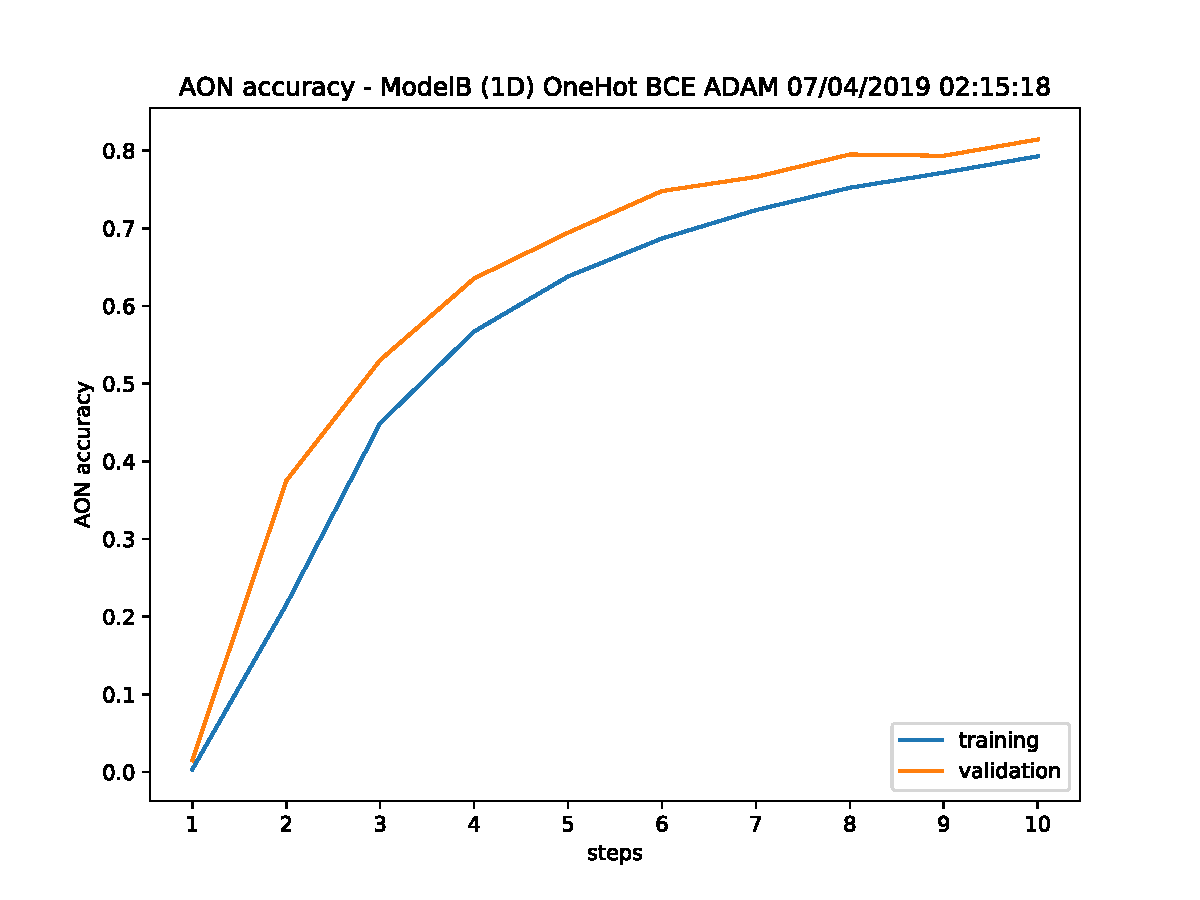
\includegraphics[width=0.45\textwidth]{figures/training_plots/ModelB-(1D)-OneHot-BCE-ADAM_07-04-2019_02-15-18_AON-accuracy.pdf} & 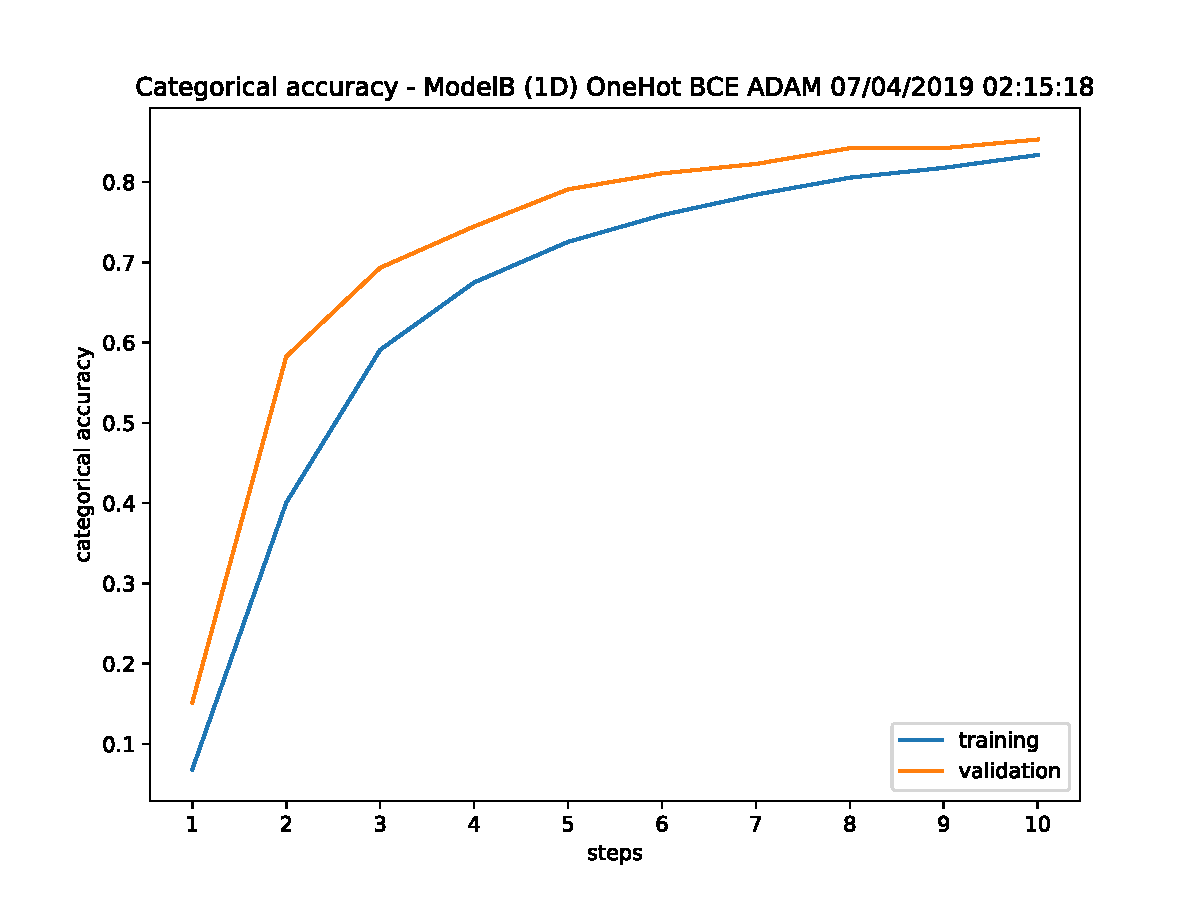
\includegraphics[width=0.45\textwidth]{figures/training_plots/ModelB-(1D)-OneHot-BCE-ADAM_07-04-2019_02-15-18_categorical-accuracy.pdf} \\
                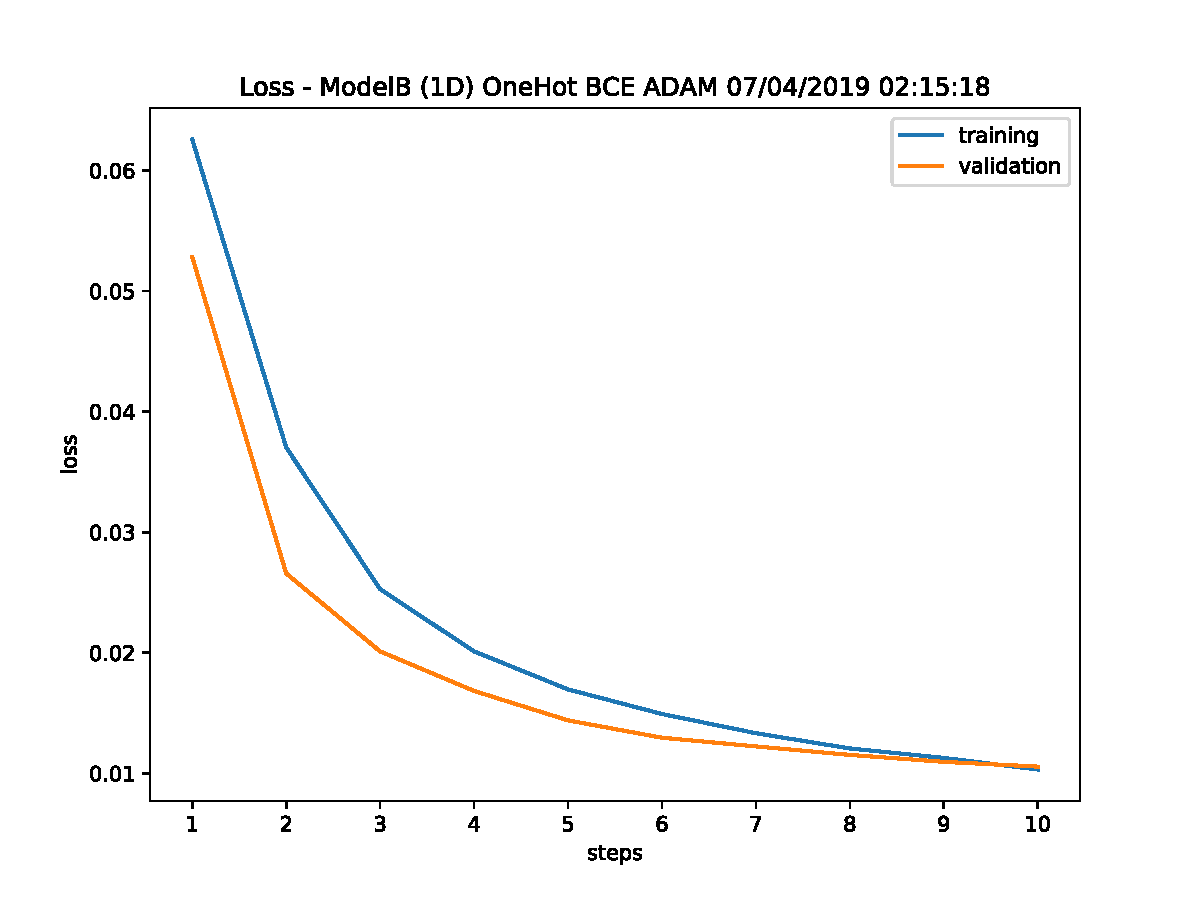
\includegraphics[width=0.45\textwidth]{figures/training_plots/ModelB-(1D)-OneHot-BCE-ADAM_07-04-2019_02-15-18_loss.pdf} & 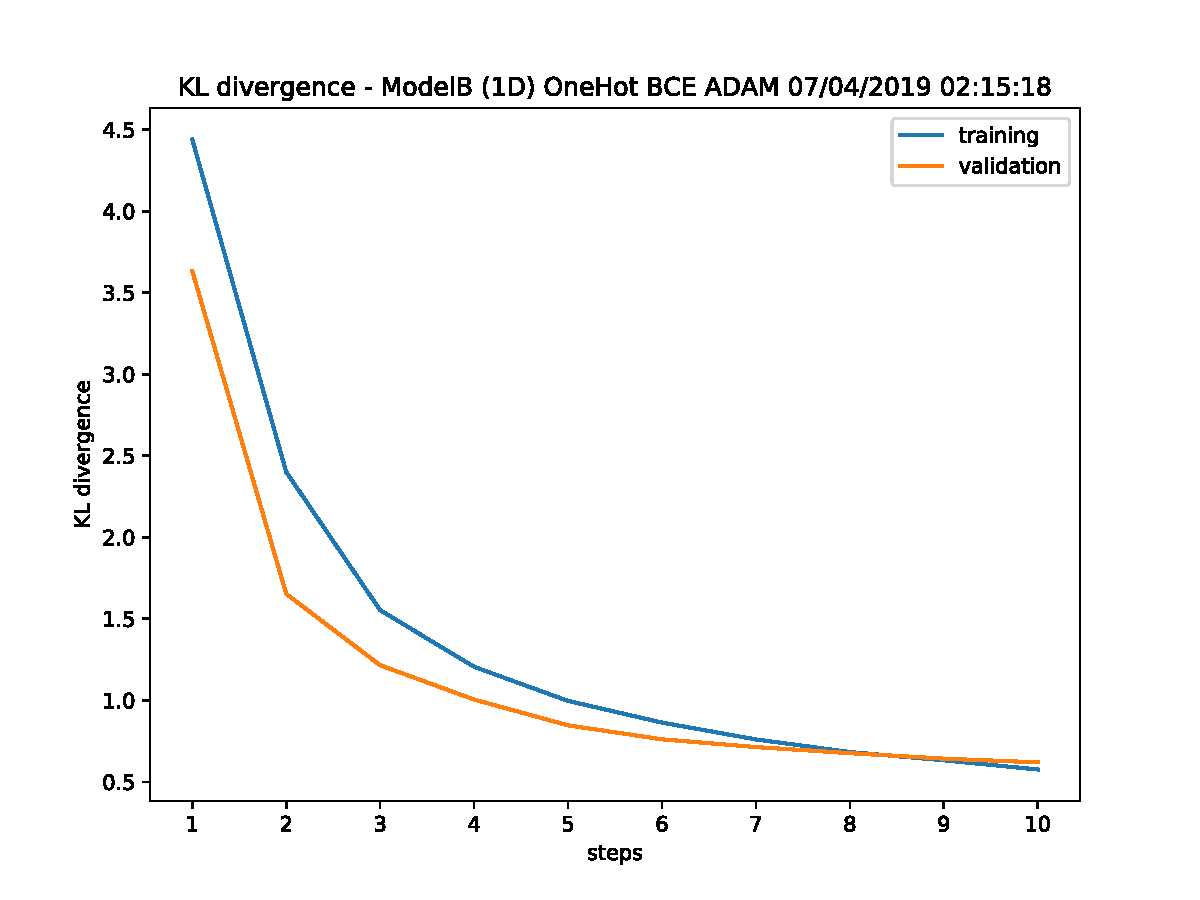
\includegraphics[width=0.45\textwidth]{figures/training_plots/ModelB-(1D)-OneHot-BCE-ADAM_07-04-2019_02-15-18_KL-divergence.pdf}
            \end{tabular}
            \caption*{One-hot encoding, BCE loss}
        \end{figure}
        
        \begin{figure}[H]
            \centering
            \begin{tabular}{cc}
                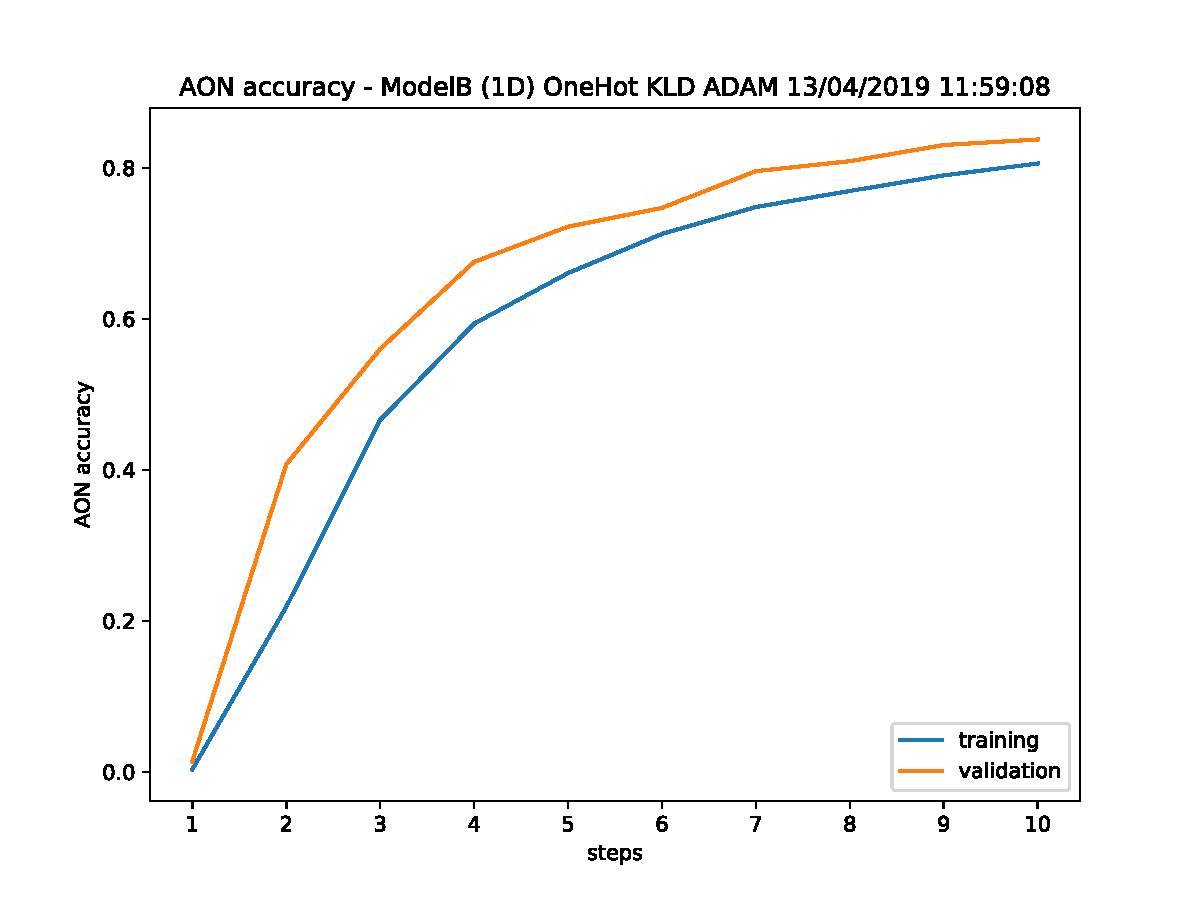
\includegraphics[width=0.45\textwidth]{figures/training_plots/ModelB-(1D)-OneHot-KLD-ADAM_13-04-2019_11-59-08_AON-accuracy.pdf} & 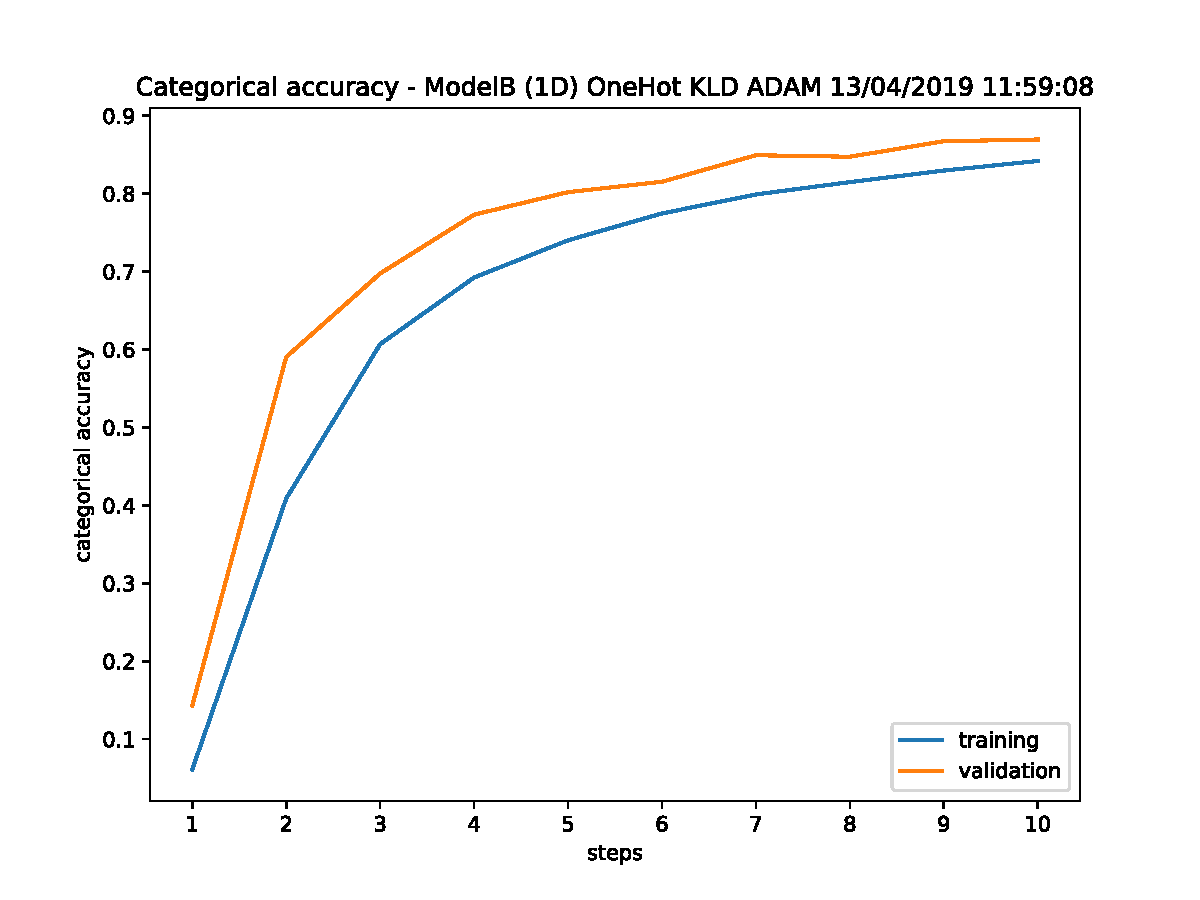
\includegraphics[width=0.45\textwidth]{figures/training_plots/ModelB-(1D)-OneHot-KLD-ADAM_13-04-2019_11-59-08_categorical-accuracy.pdf} \\
                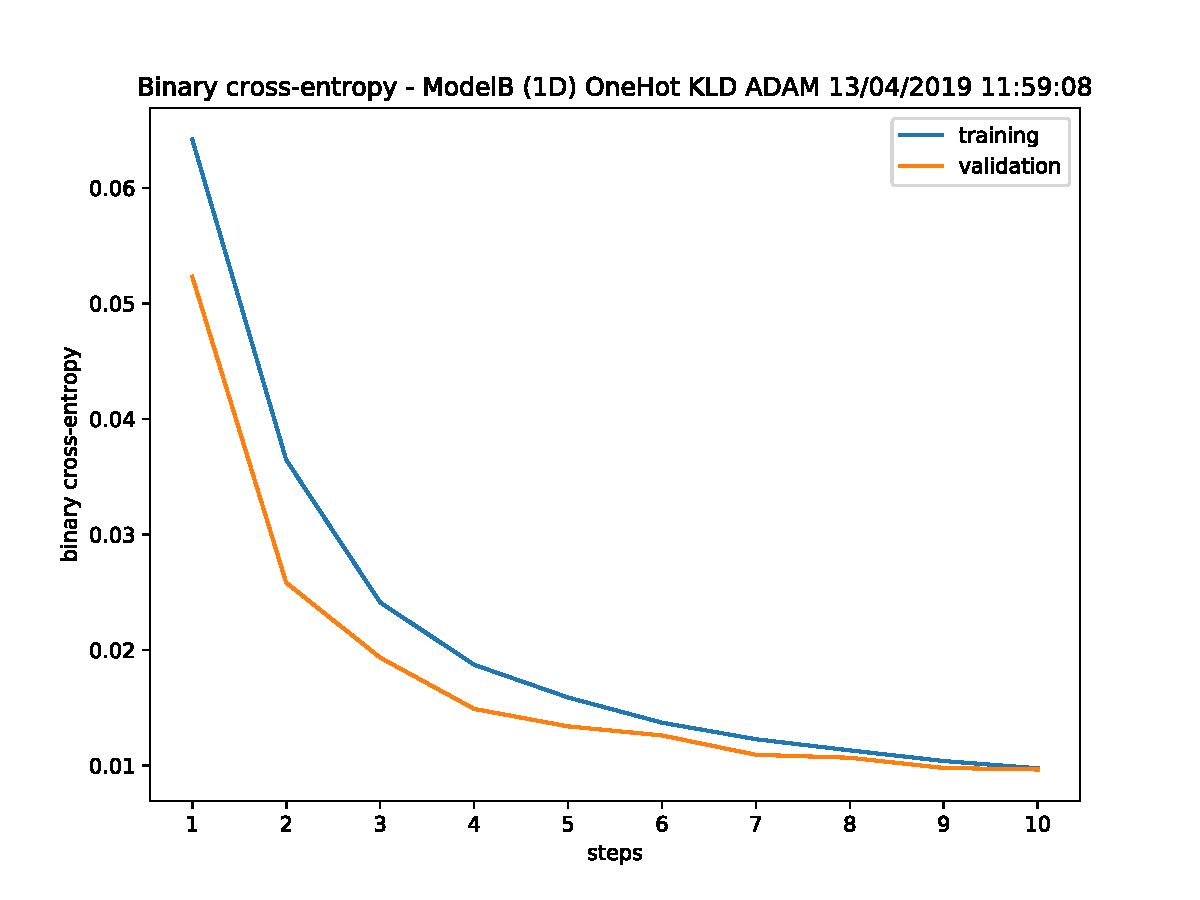
\includegraphics[width=0.45\textwidth]{figures/training_plots/ModelB-(1D)-OneHot-KLD-ADAM_13-04-2019_11-59-08_binary-cross-entropy.pdf} & 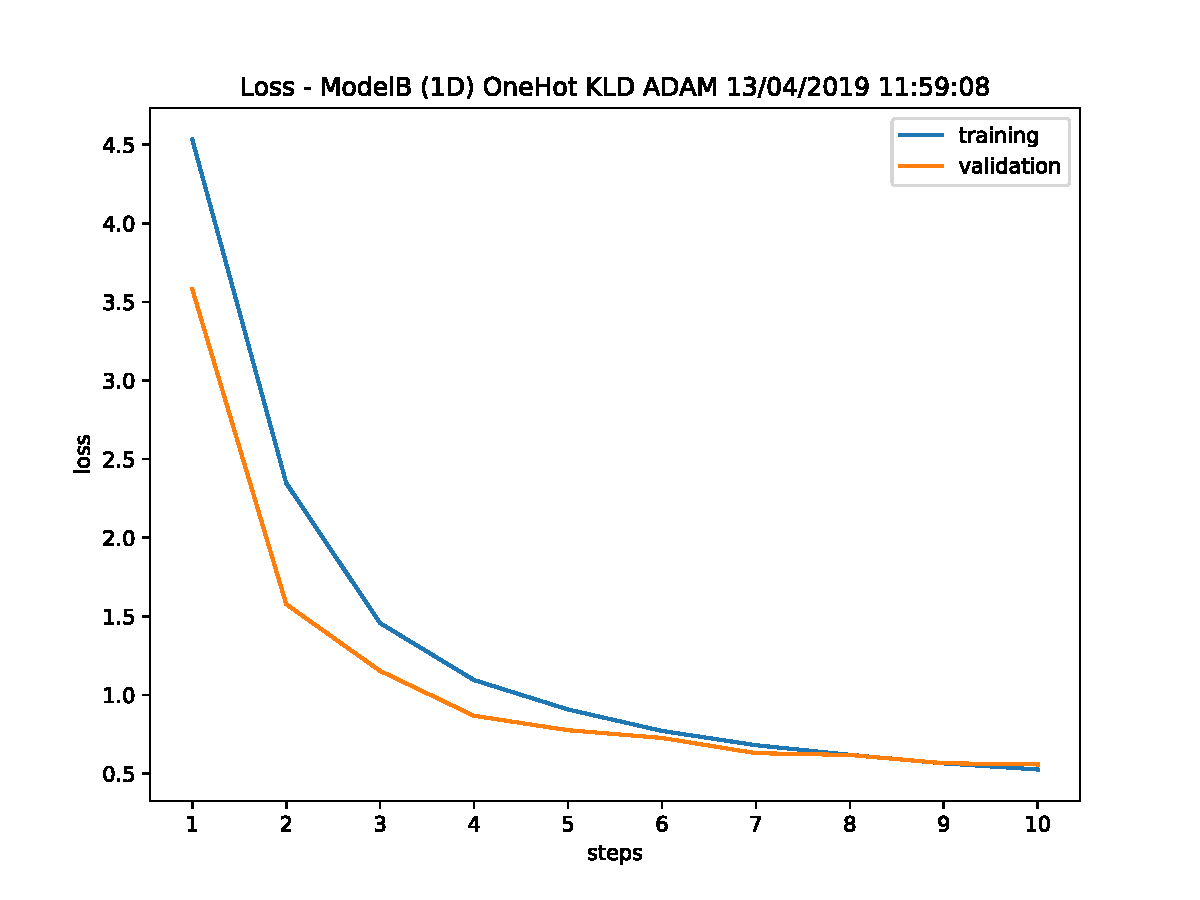
\includegraphics[width=0.45\textwidth]{figures/training_plots/ModelB-(1D)-OneHot-KLD-ADAM_13-04-2019_11-59-08_loss.pdf}
            \end{tabular}
            \caption*{One-hot encoding, KLD loss}
        \end{figure}
        
        \begin{figure}[H]
            \centering
            \begin{tabular}{cc}
                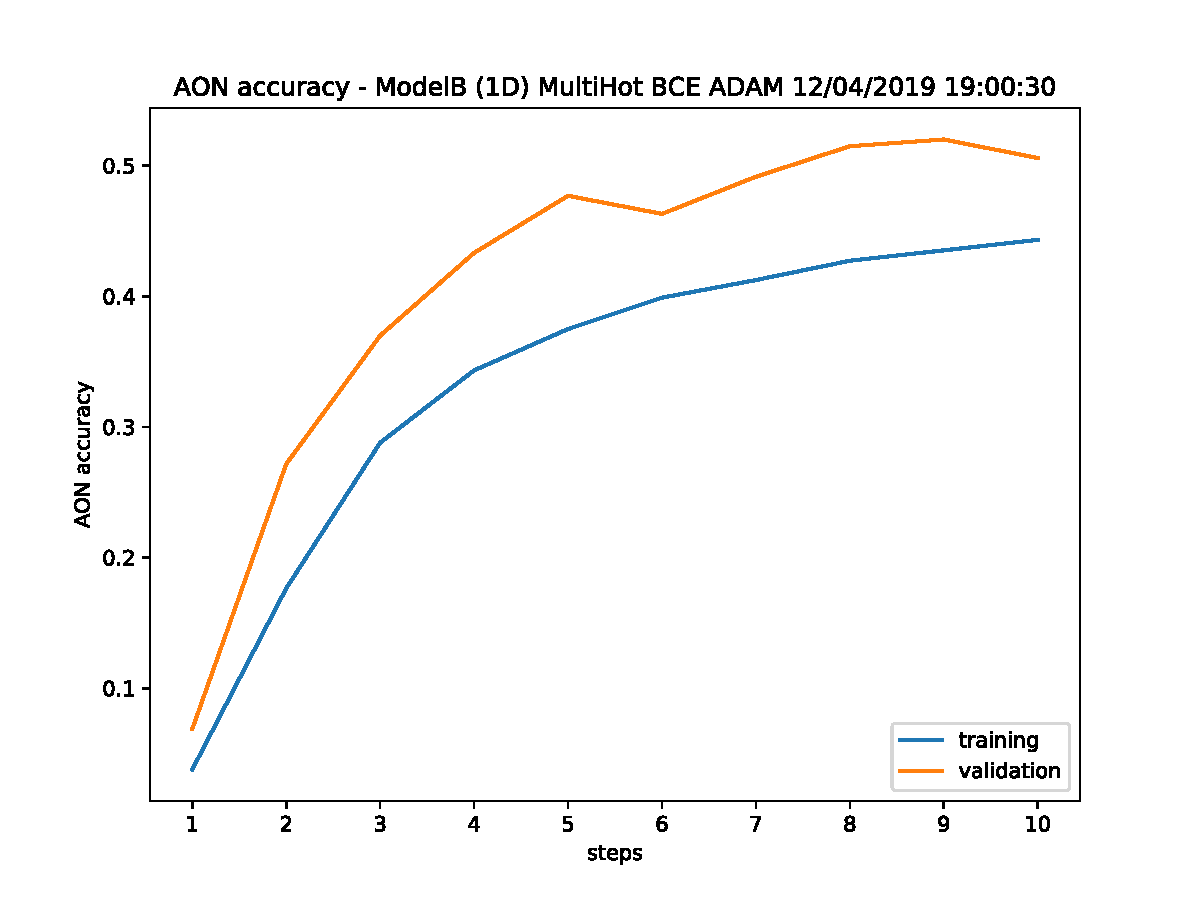
\includegraphics[width=0.48\textwidth]{figures/training_plots/ModelB-(1D)-MultiHot-BCE-ADAM_12-04-2019_19-00-30_AON-accuracy.pdf} & 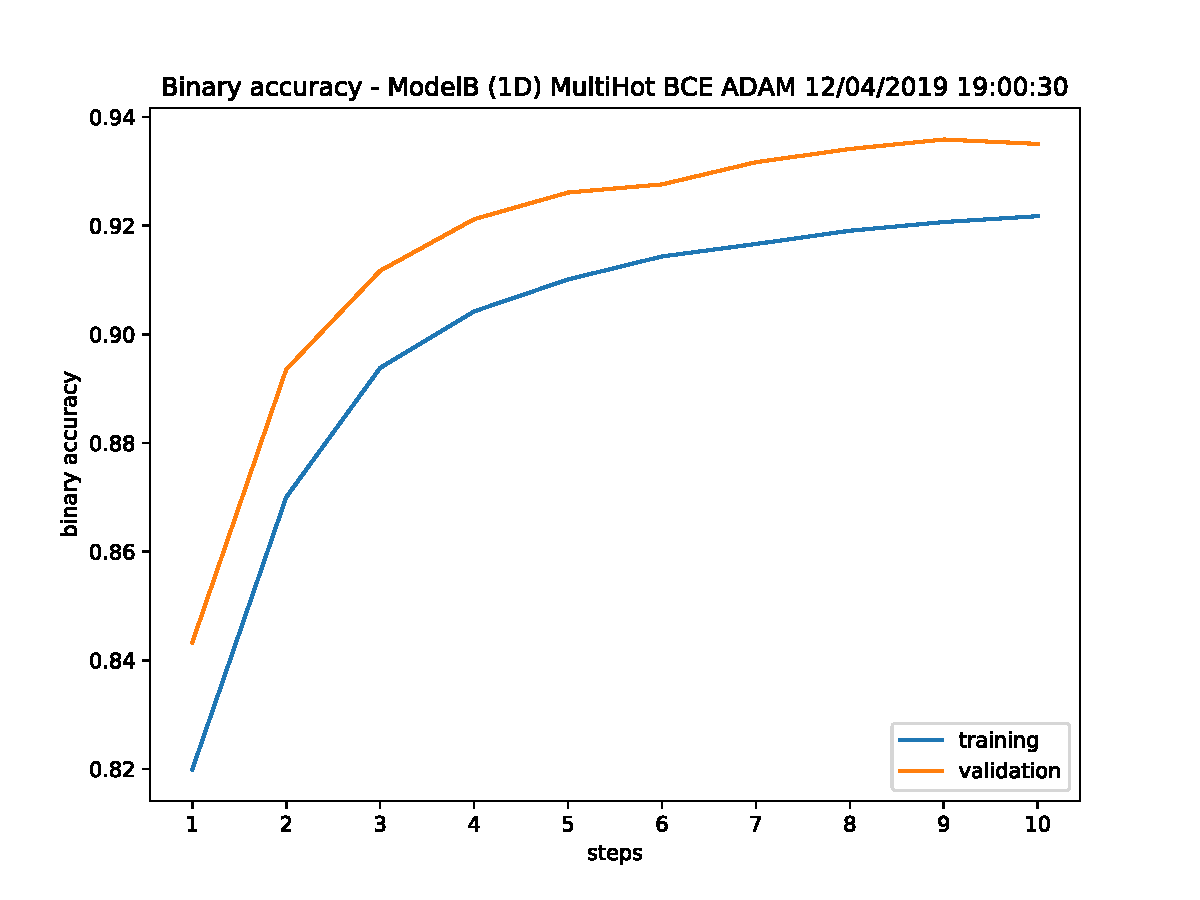
\includegraphics[width=0.48\textwidth]{figures/training_plots/ModelB-(1D)-MultiHot-BCE-ADAM_12-04-2019_19-00-30_binary-accuracy.pdf} \\
                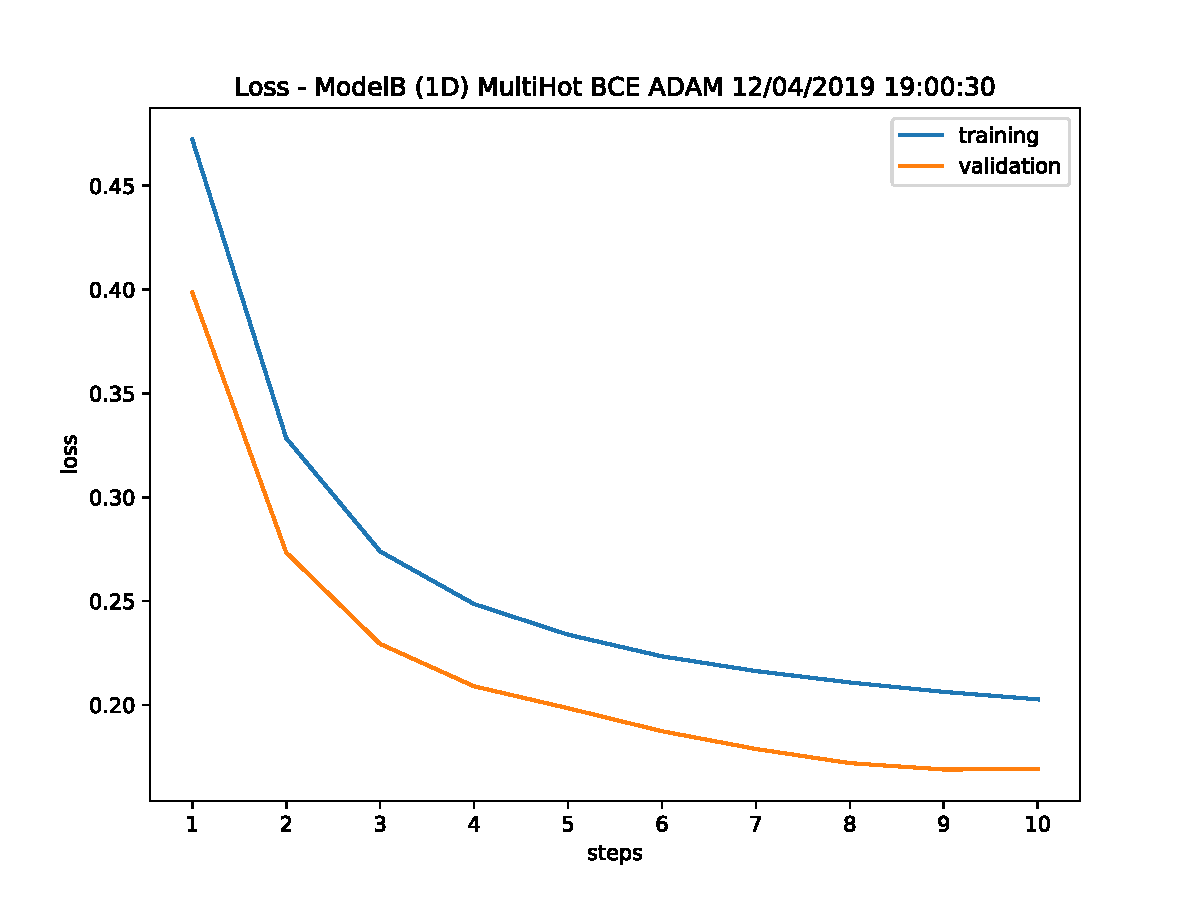
\includegraphics[width=0.48\textwidth]{figures/training_plots/ModelB-(1D)-MultiHot-BCE-ADAM_12-04-2019_19-00-30_loss.pdf} & 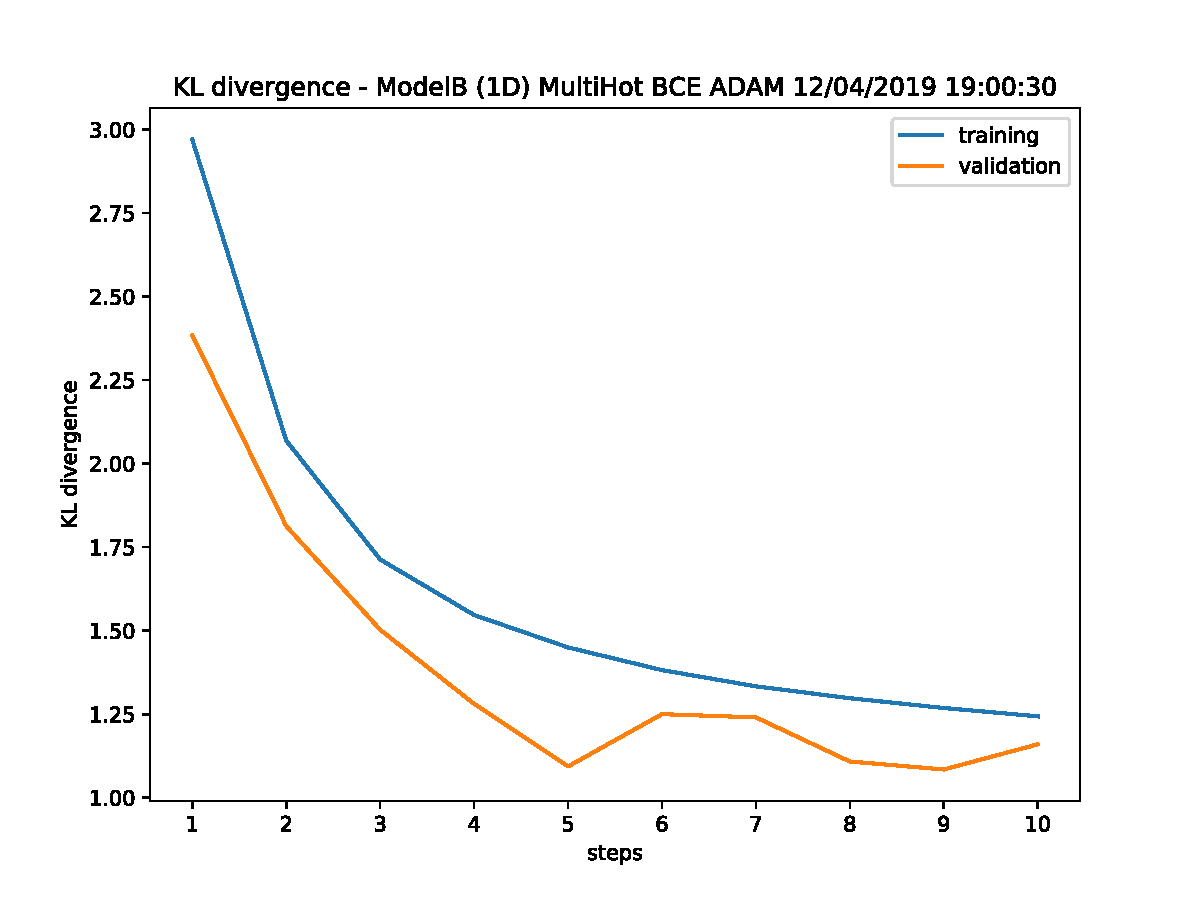
\includegraphics[width=0.48\textwidth]{figures/training_plots/ModelB-(1D)-MultiHot-BCE-ADAM_12-04-2019_19-00-30_KL-divergence.pdf}
            \end{tabular}
            \caption*{Multi-hot encoding, BCE loss}
        \end{figure}
        
        \begin{figure}[H]
            \centering
            \begin{tabular}{cc}
                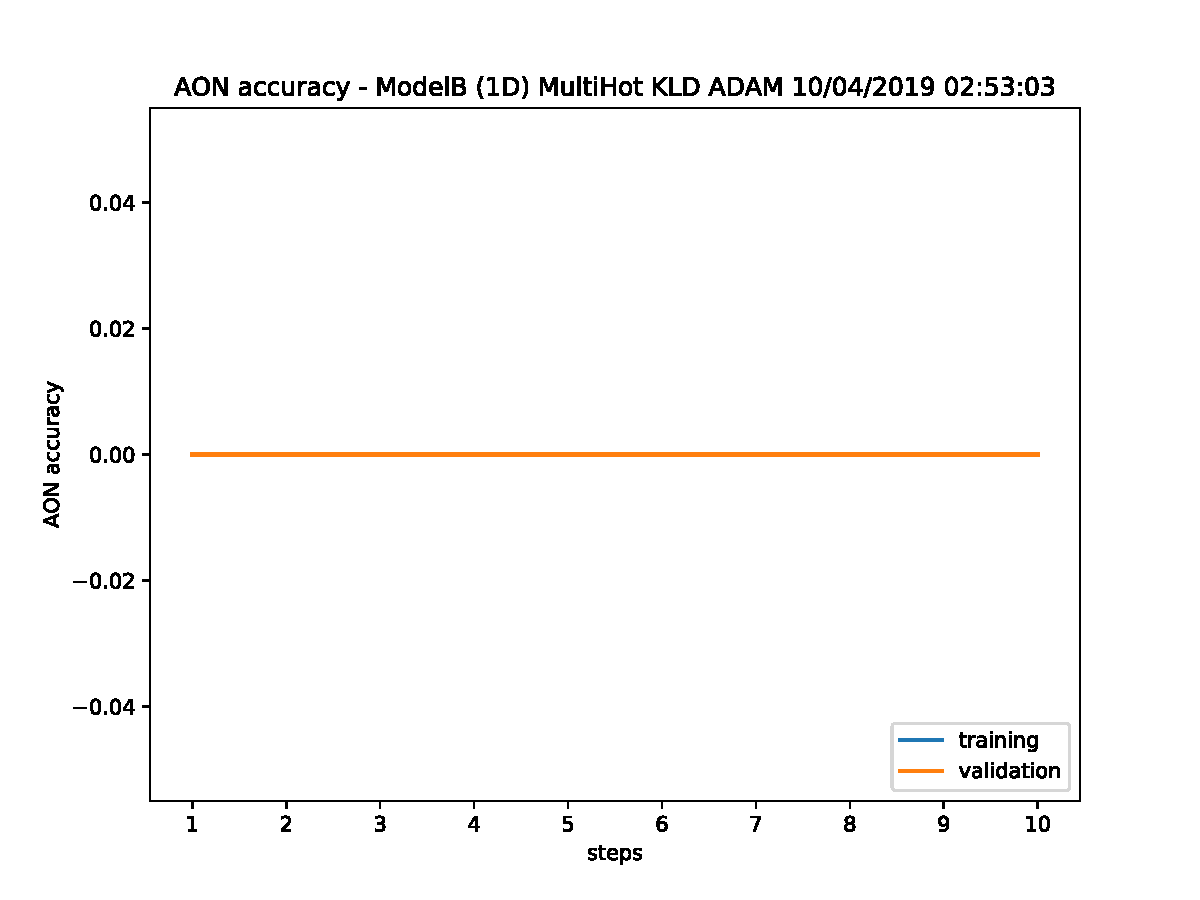
\includegraphics[width=0.48\textwidth]{figures/training_plots/ModelB-(1D)-MultiHot-KLD-ADAM_10-04-2019_02-53-03_AON-accuracy.pdf} & 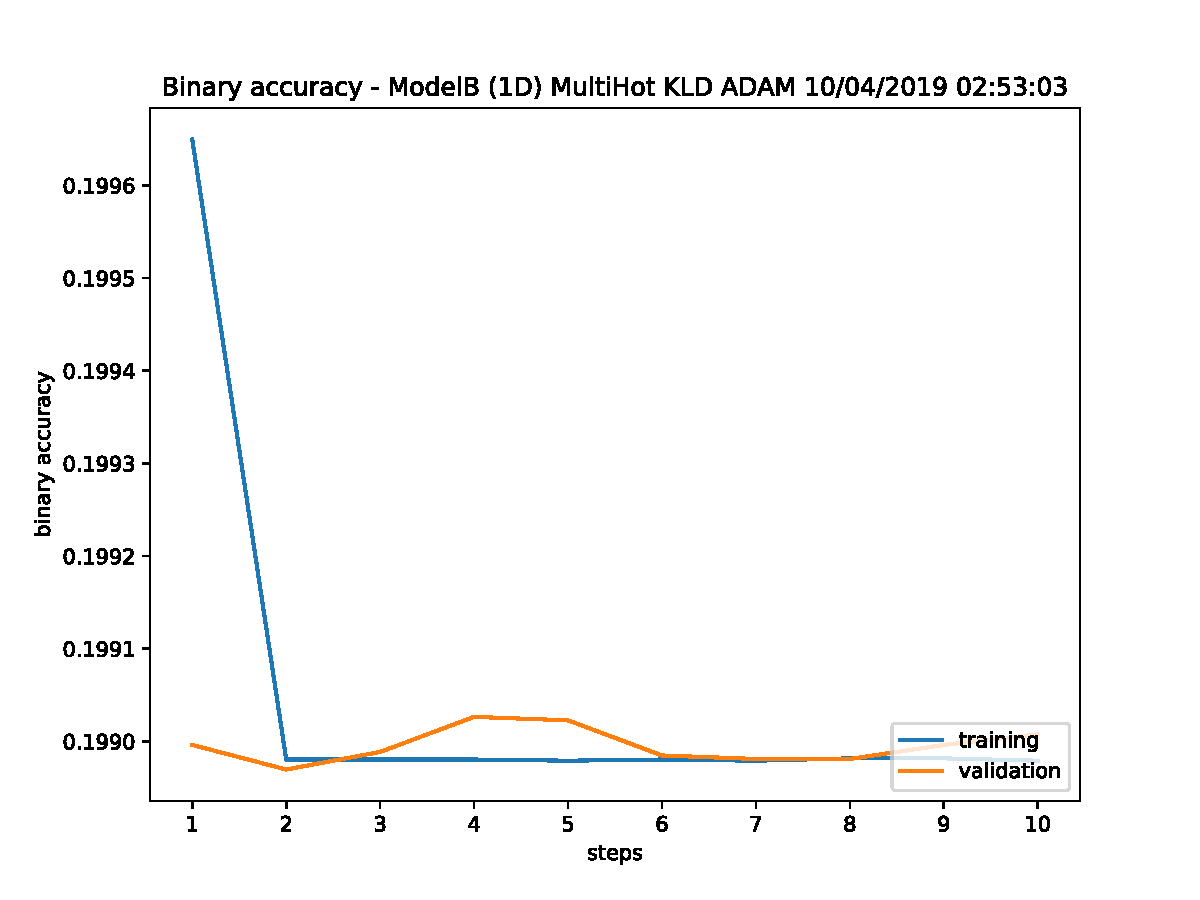
\includegraphics[width=0.48\textwidth]{figures/training_plots/ModelB-(1D)-MultiHot-KLD-ADAM_10-04-2019_02-53-03_binary-accuracy.pdf} \\
                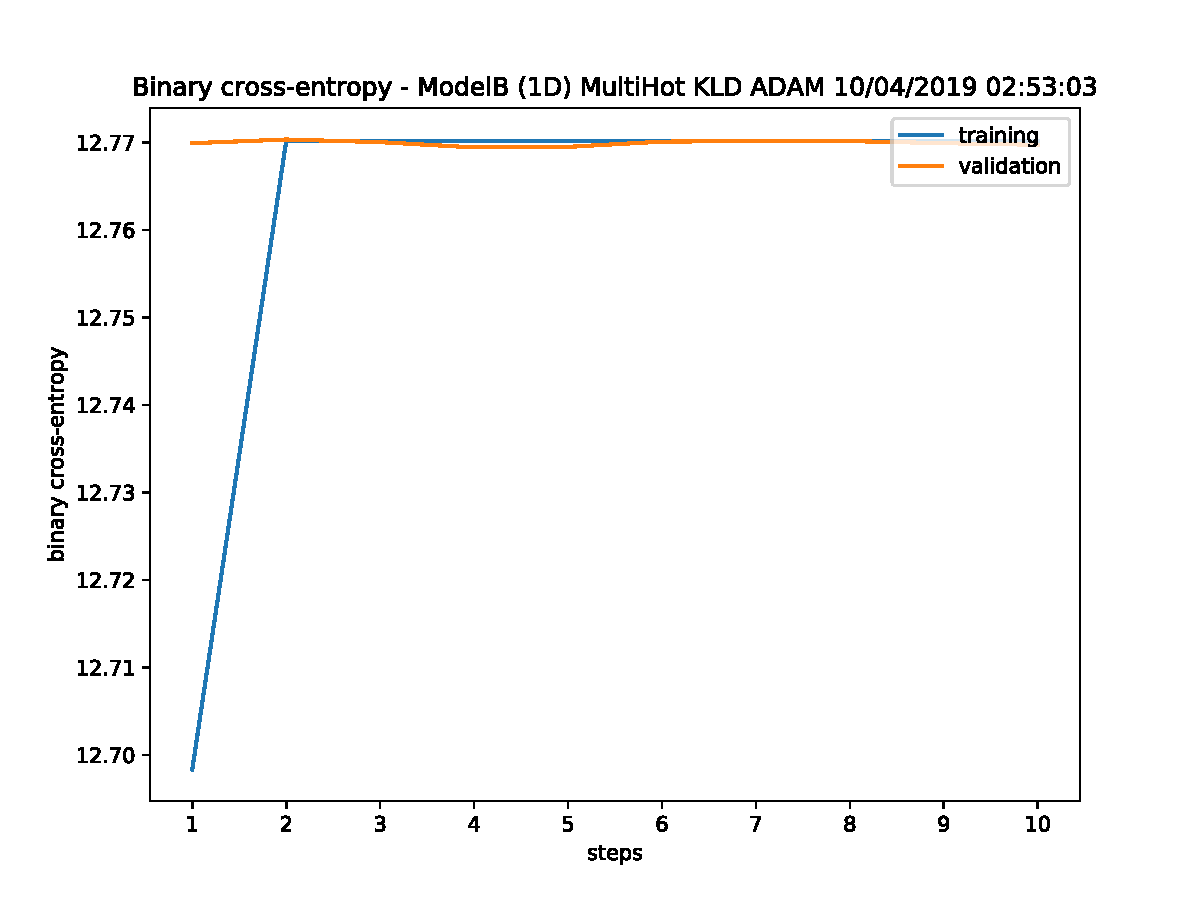
\includegraphics[width=0.48\textwidth]{figures/training_plots/ModelB-(1D)-MultiHot-KLD-ADAM_10-04-2019_02-53-03_binary-cross-entropy.pdf} & 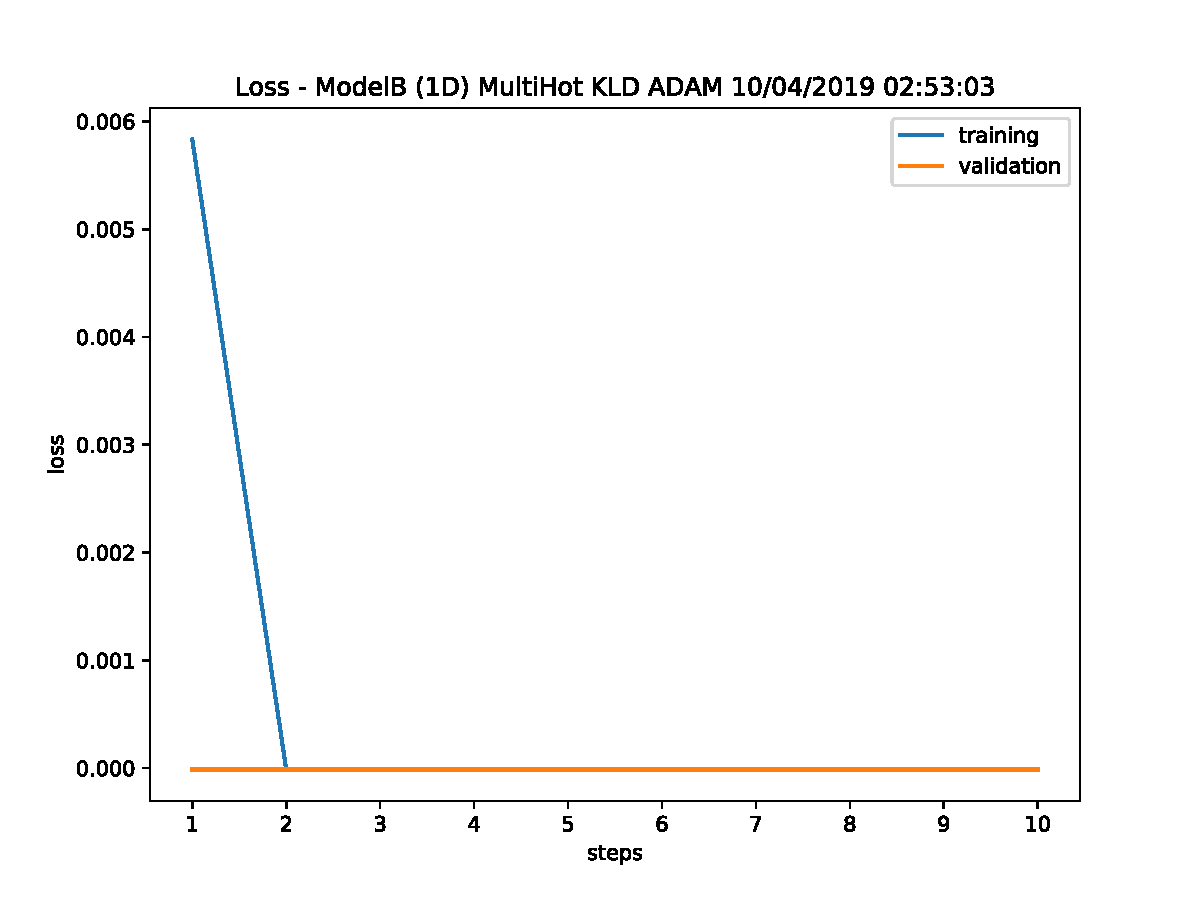
\includegraphics[width=0.48\textwidth]{figures/training_plots/ModelB-(1D)-MultiHot-KLD-ADAM_10-04-2019_02-53-03_loss.pdf}
            \end{tabular}
            \caption*{Multi-hot encoding, KLD loss}
        \end{figure}
        
        \subsection{Model C training metrics}
        \label{app:modelC_training}
        \texttt{Referred to in section \ref{sec:training_analysis_modelC}}
        \begin{figure}[H]
            \centering
            \begin{tabular}{cc}
                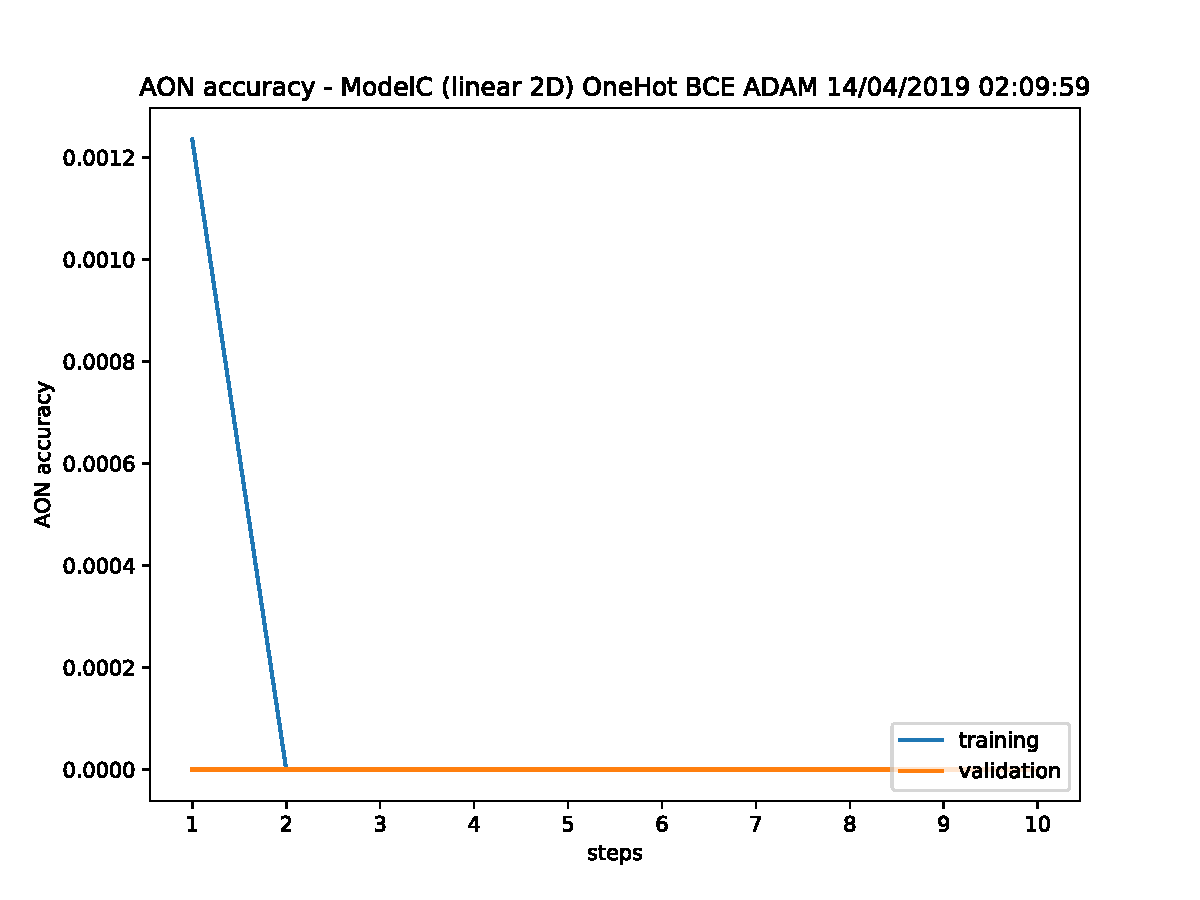
\includegraphics[width=0.45\textwidth]{figures/training_plots/ModelC-(linear_2D)-OneHot-BCE-ADAM_14-04-2019_02-09-59_AON-accuracy.pdf} & 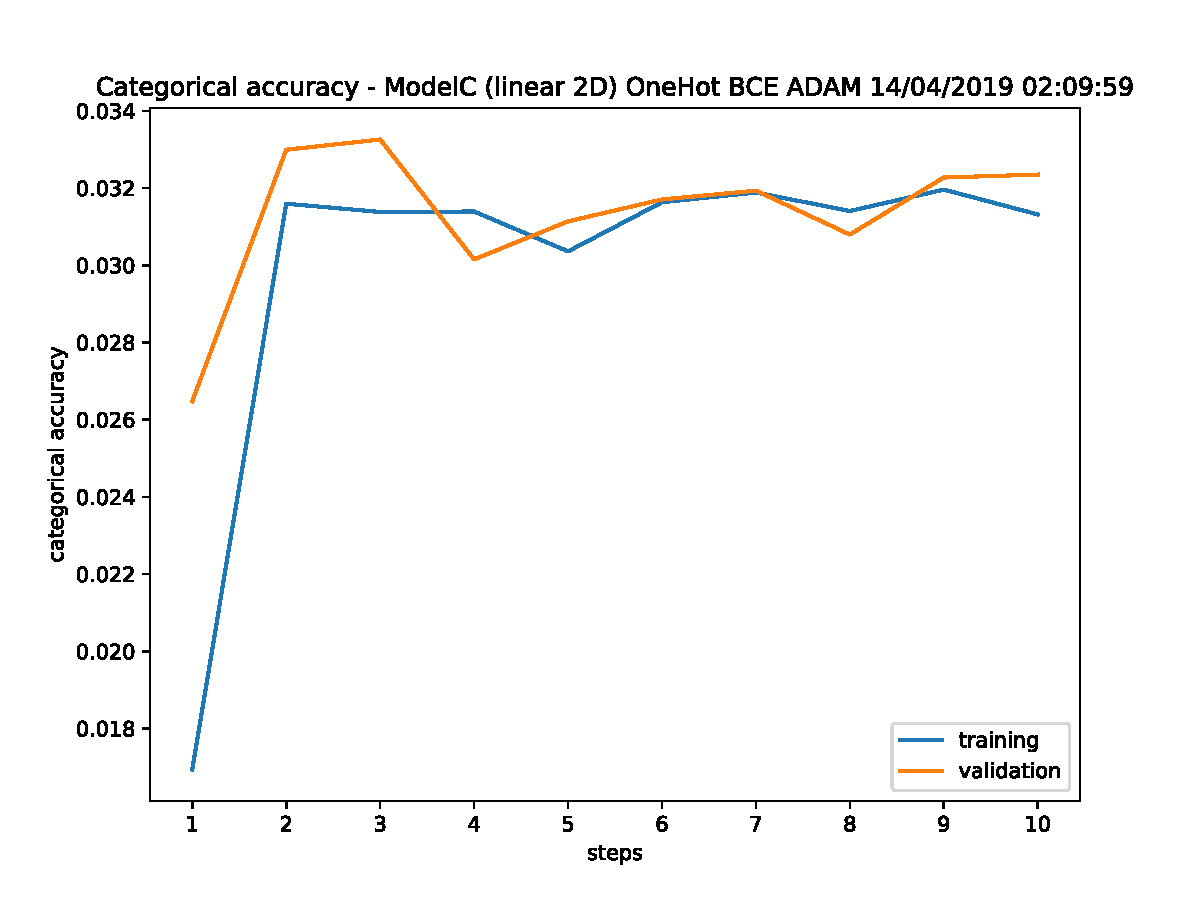
\includegraphics[width=0.45\textwidth]{figures/training_plots/ModelC-(linear_2D)-OneHot-BCE-ADAM_14-04-2019_02-09-59_categorical-accuracy.pdf} \\
                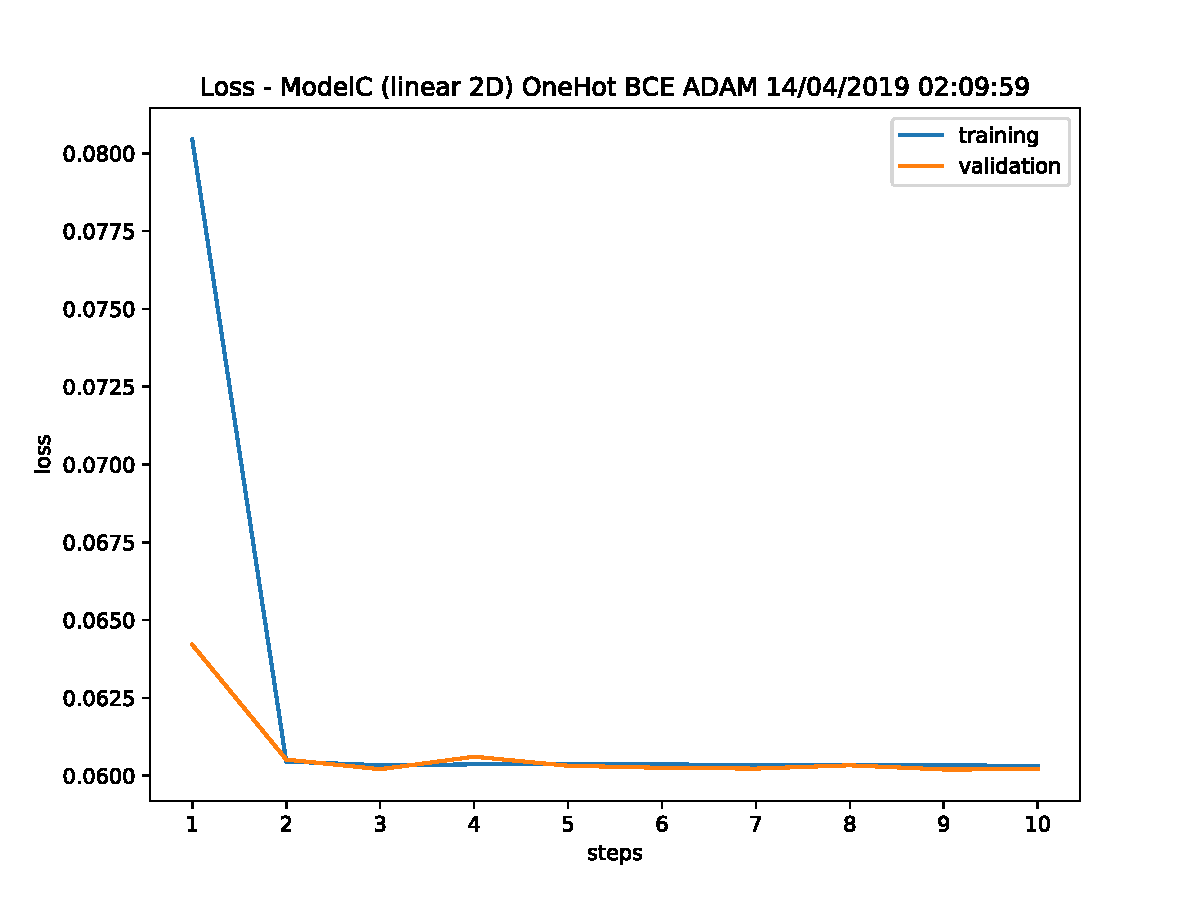
\includegraphics[width=0.45\textwidth]{figures/training_plots/ModelC-(linear_2D)-OneHot-BCE-ADAM_14-04-2019_02-09-59_loss.pdf} & 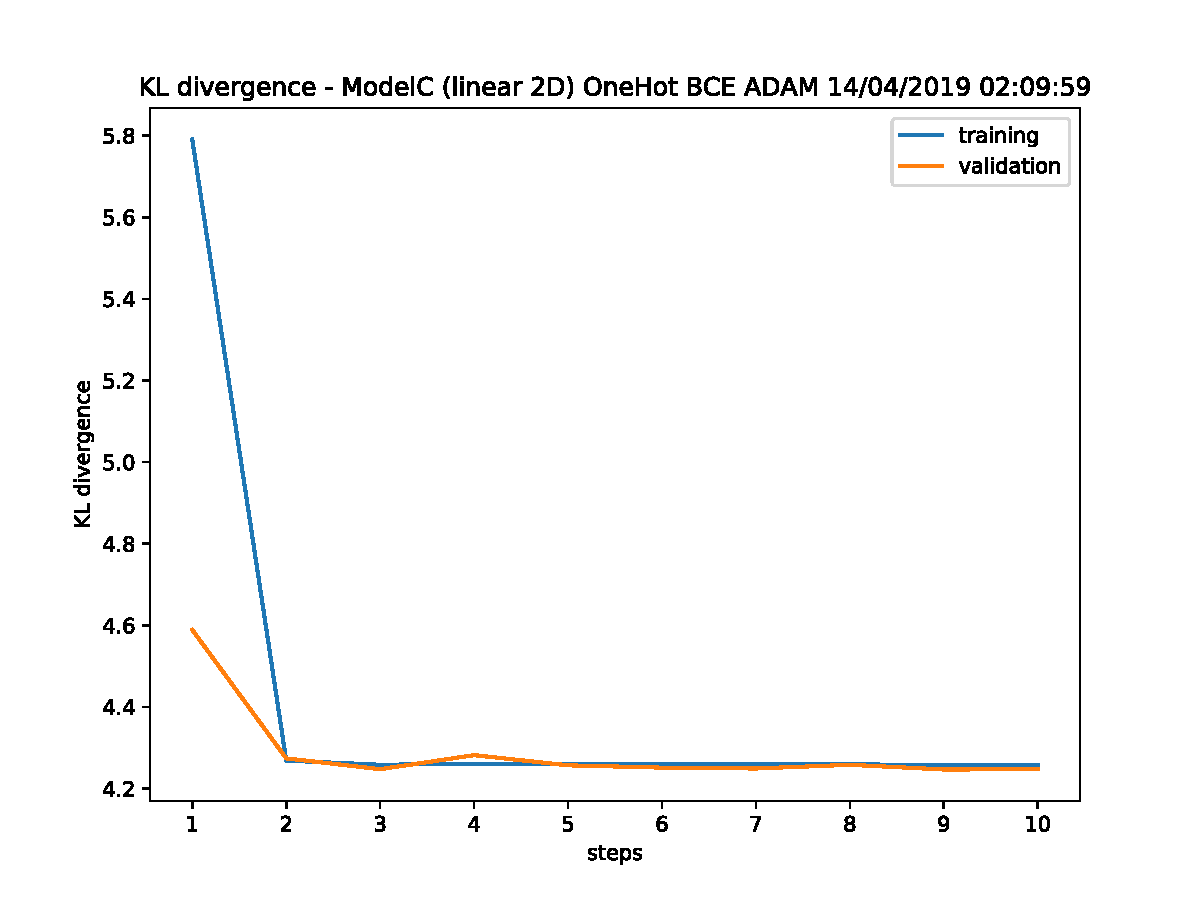
\includegraphics[width=0.45\textwidth]{figures/training_plots/ModelC-(linear_2D)-OneHot-BCE-ADAM_14-04-2019_02-09-59_KL-divergence.pdf}
            \end{tabular}
            \caption*{Linear magnitude, one-hot encoding, BCE loss}
        \end{figure}
        
        \begin{figure}[H]
            \centering
            \begin{tabular}{cc}
                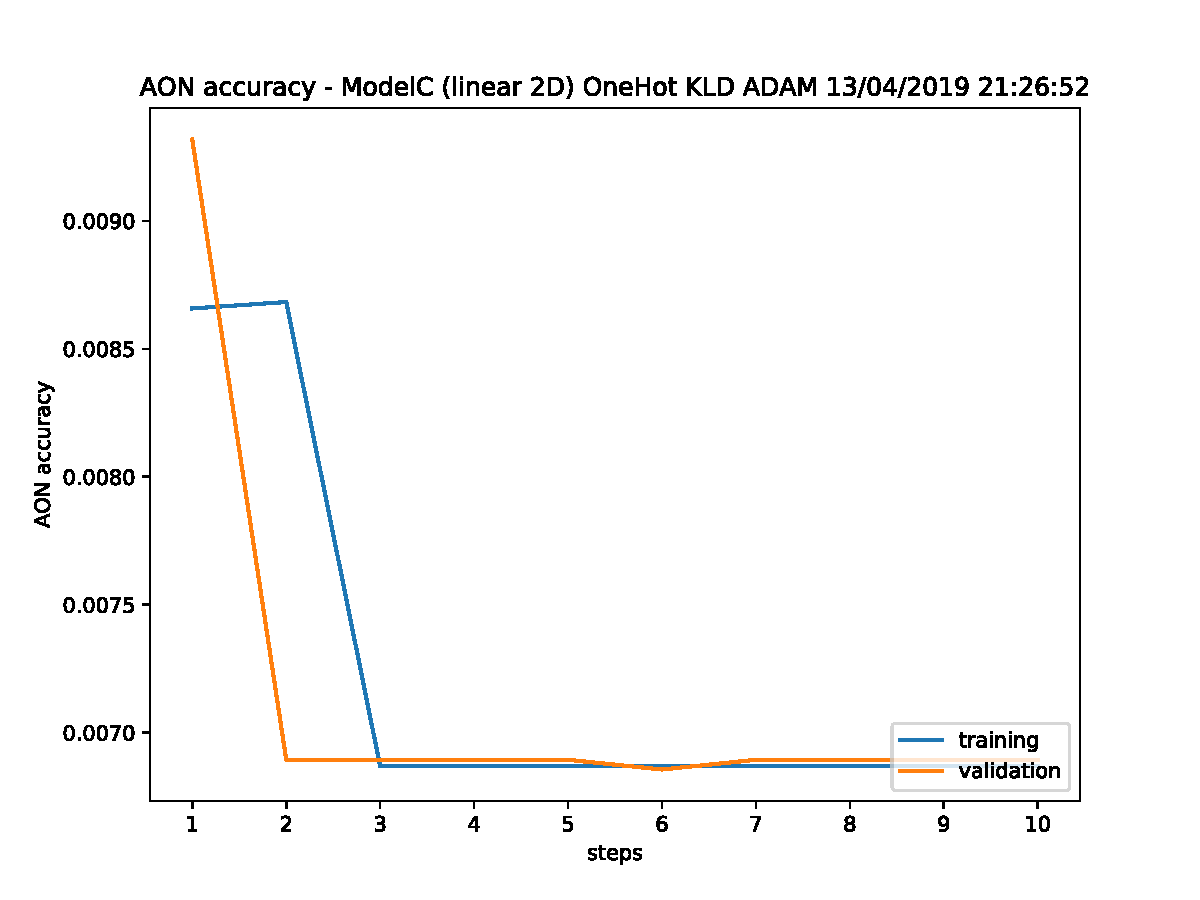
\includegraphics[width=0.45\textwidth]{figures/training_plots/ModelC-(linear_2D)-OneHot-KLD-ADAM_13-04-2019_21-26-52_AON-accuracy.pdf} & 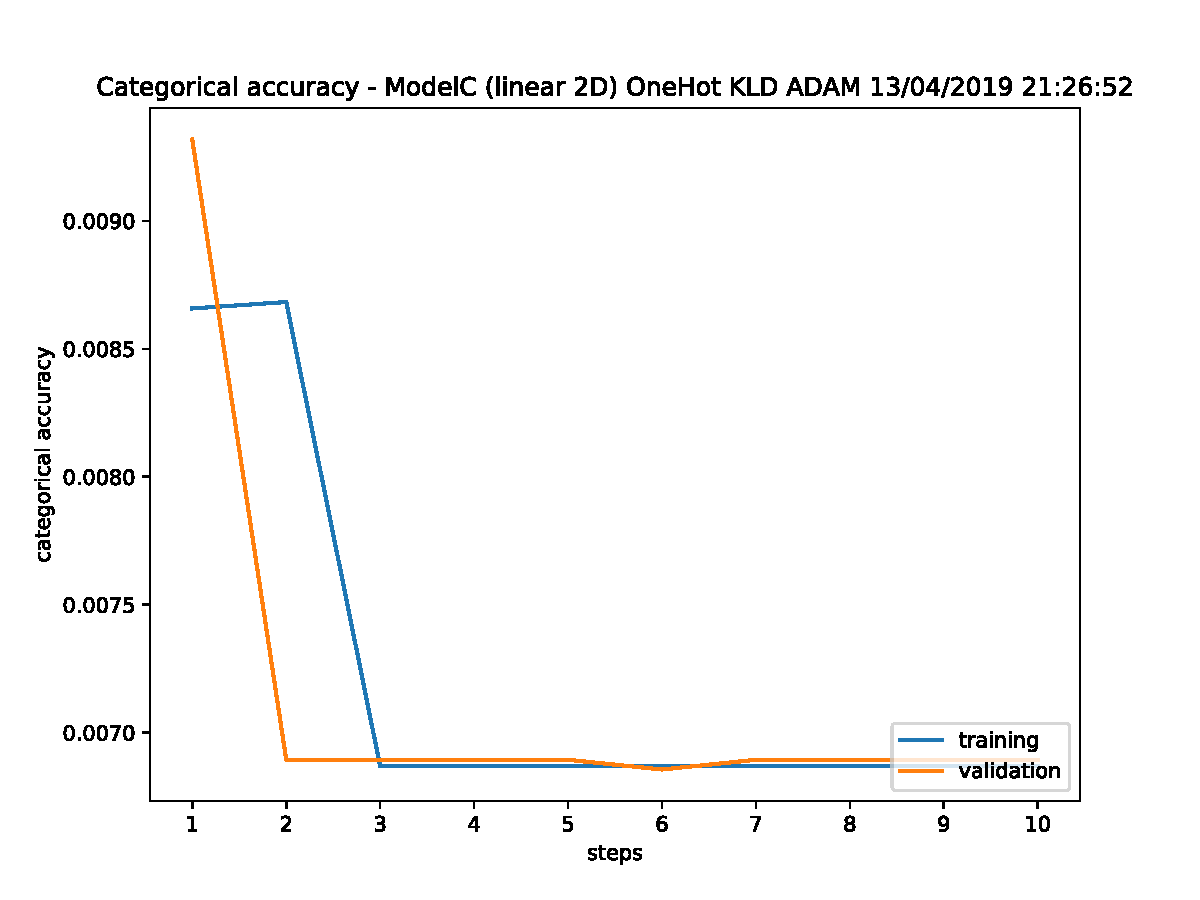
\includegraphics[width=0.45\textwidth]{figures/training_plots/ModelC-(linear_2D)-OneHot-KLD-ADAM_13-04-2019_21-26-52_categorical-accuracy.pdf} \\
                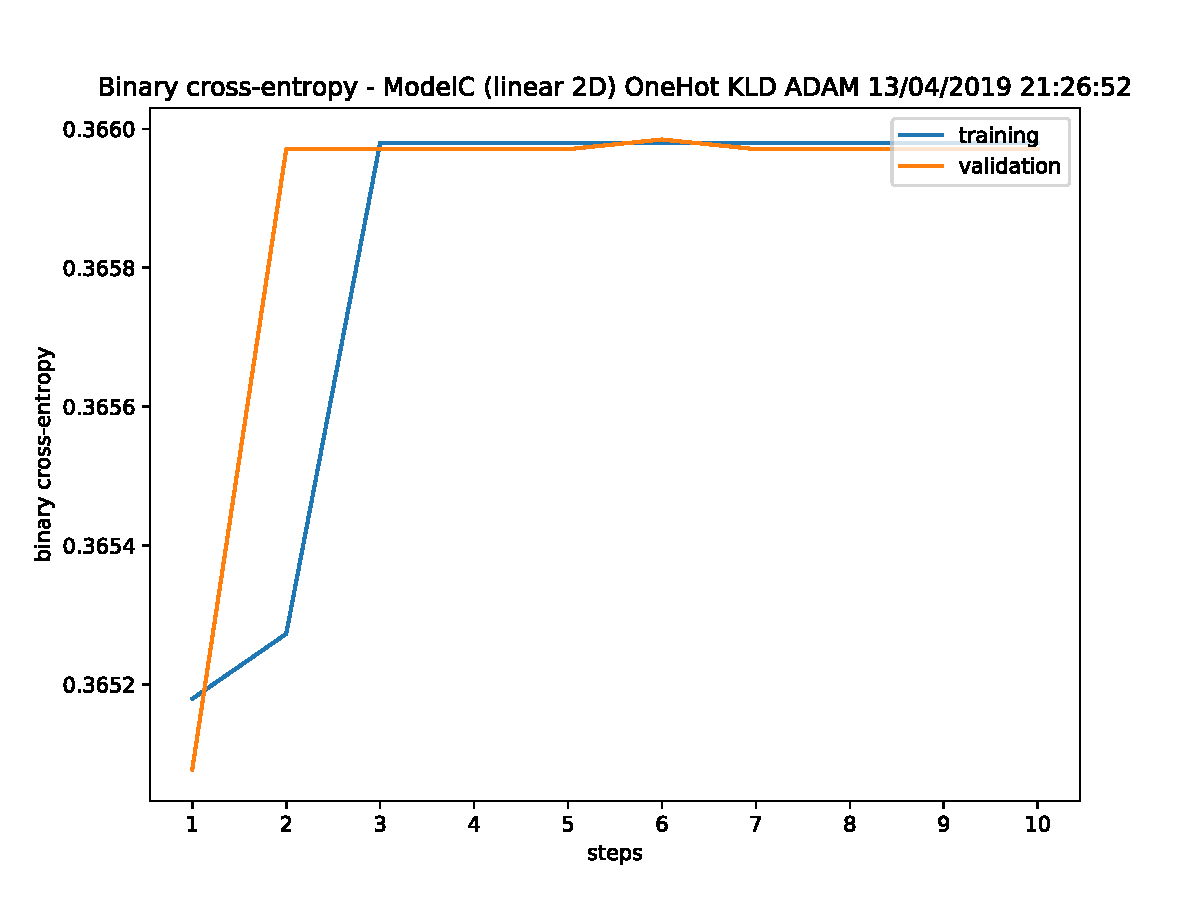
\includegraphics[width=0.45\textwidth]{figures/training_plots/ModelC-(linear_2D)-OneHot-KLD-ADAM_13-04-2019_21-26-52_binary-cross-entropy.pdf} & 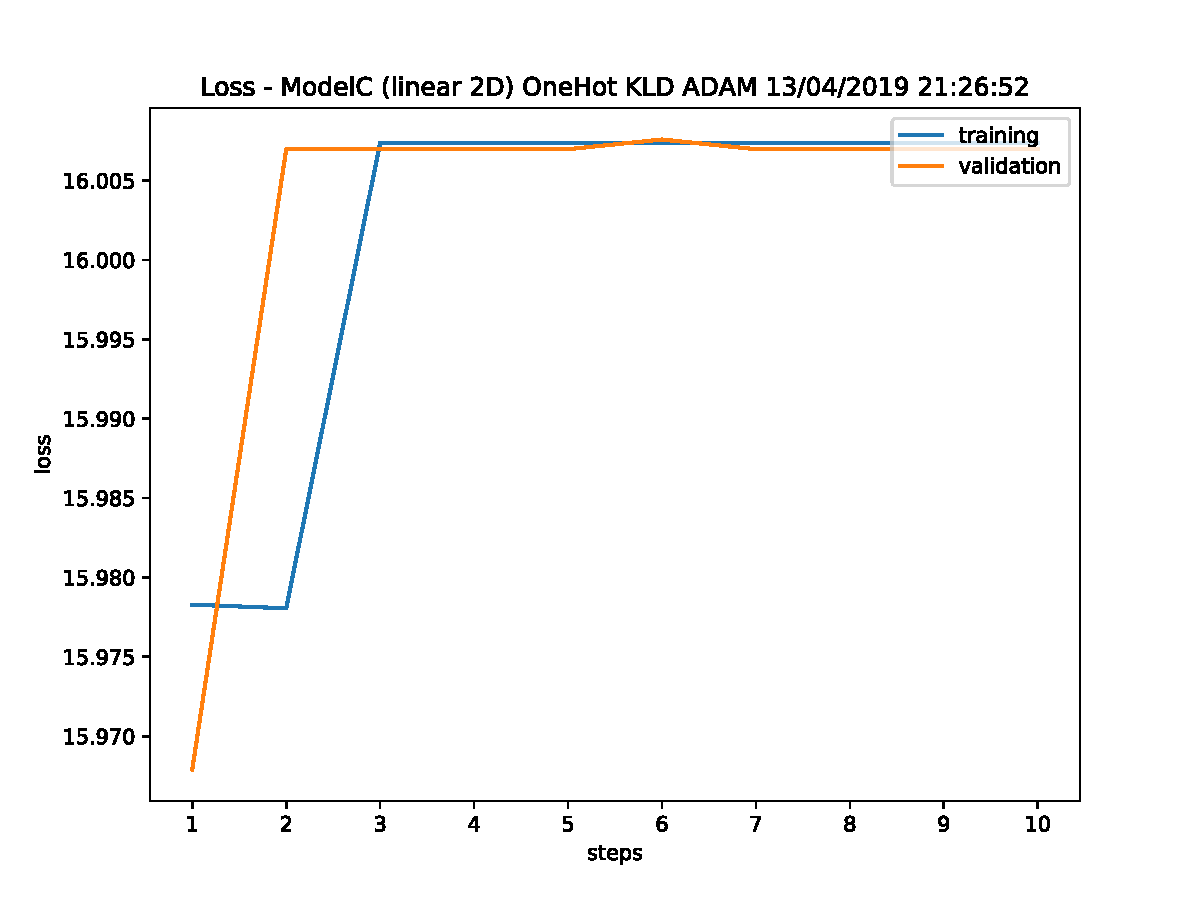
\includegraphics[width=0.45\textwidth]{figures/training_plots/ModelC-(linear_2D)-OneHot-KLD-ADAM_13-04-2019_21-26-52_loss.pdf}
            \end{tabular}
            \caption*{Linear magnitude, one-hot encoding, KLD loss}
        \end{figure}
        
        \begin{figure}[H]
            \centering
            \begin{tabular}{cc}
                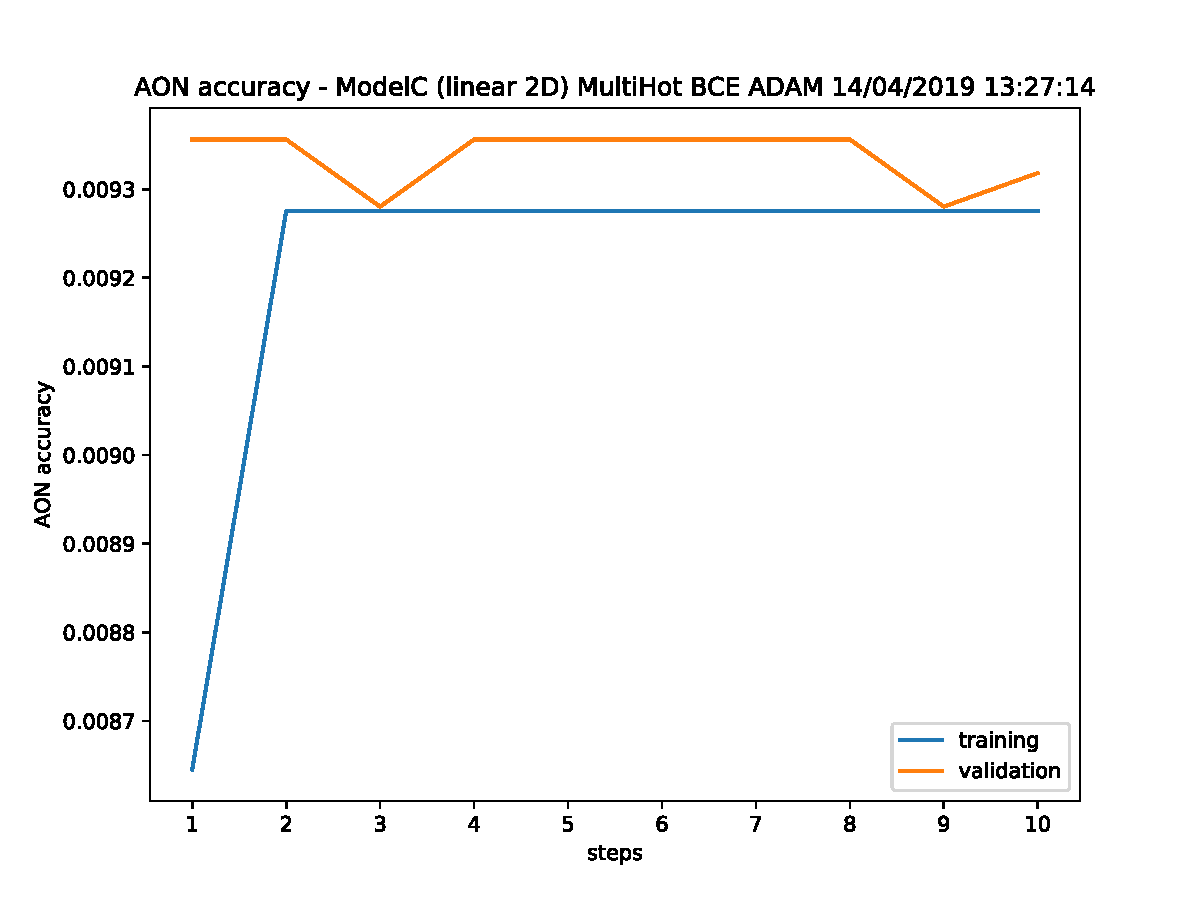
\includegraphics[width=0.48\textwidth]{figures/training_plots/ModelC-(linear_2D)-MultiHot-BCE-ADAM_14-04-2019_13-27-14_AON-accuracy.pdf} & 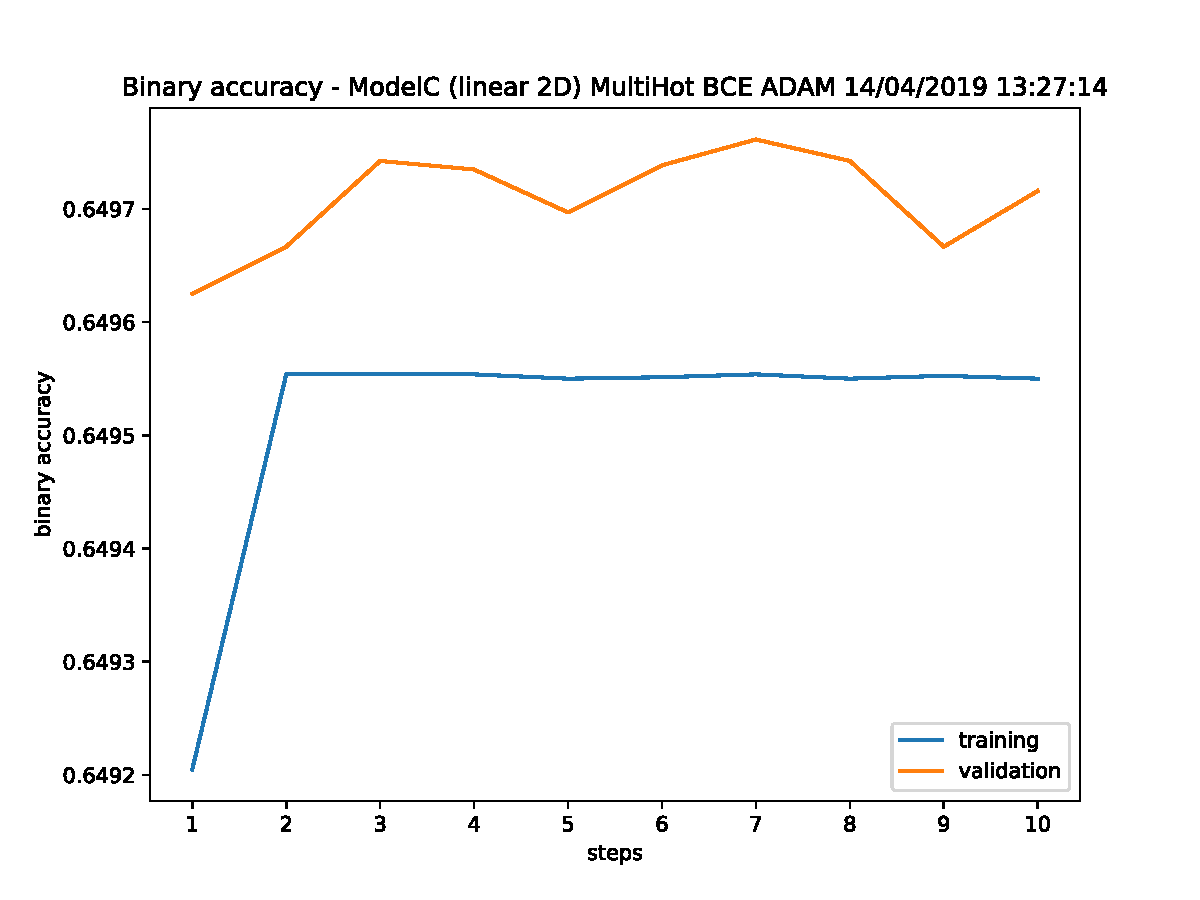
\includegraphics[width=0.48\textwidth]{figures/training_plots/ModelC-(linear_2D)-MultiHot-BCE-ADAM_14-04-2019_13-27-14_binary-accuracy.pdf} \\
                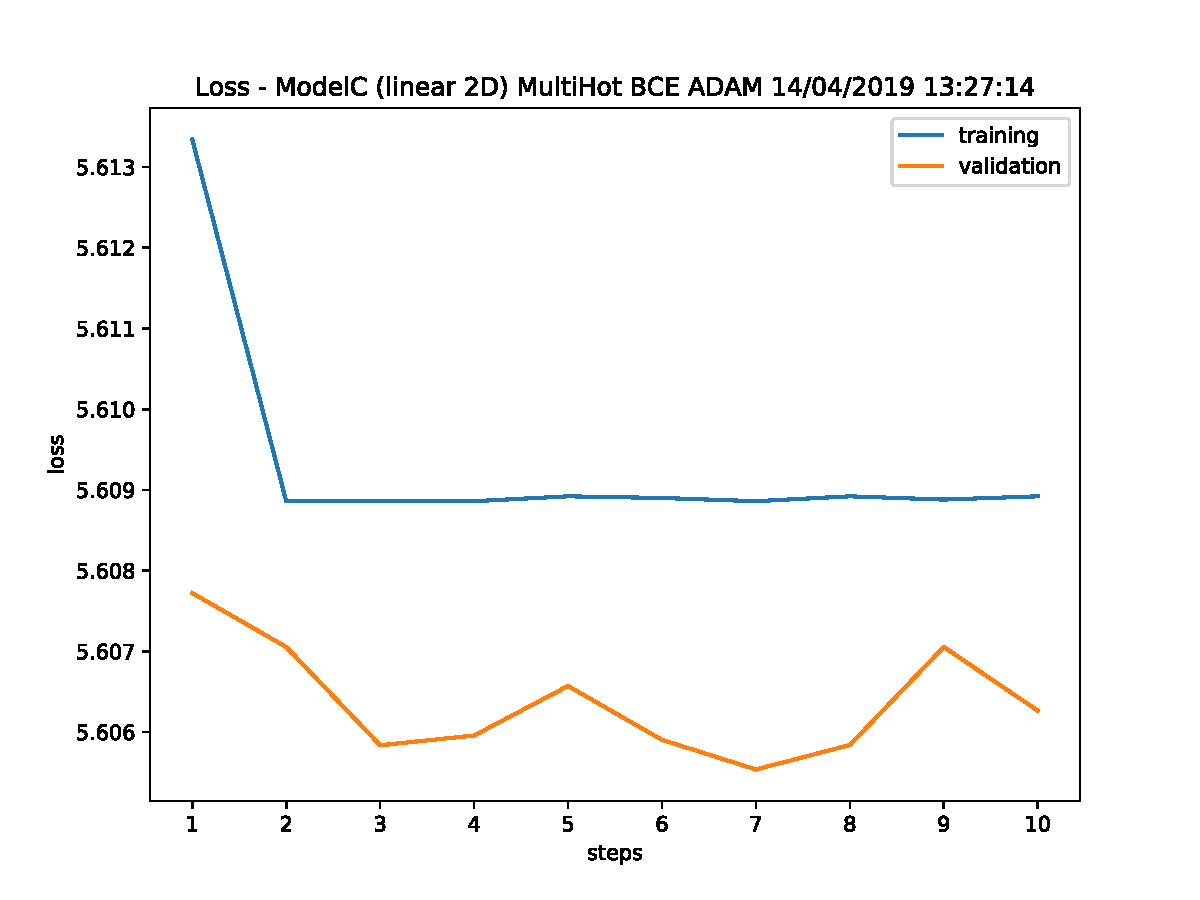
\includegraphics[width=0.48\textwidth]{figures/training_plots/ModelC-(linear_2D)-MultiHot-BCE-ADAM_14-04-2019_13-27-14_loss.pdf} & 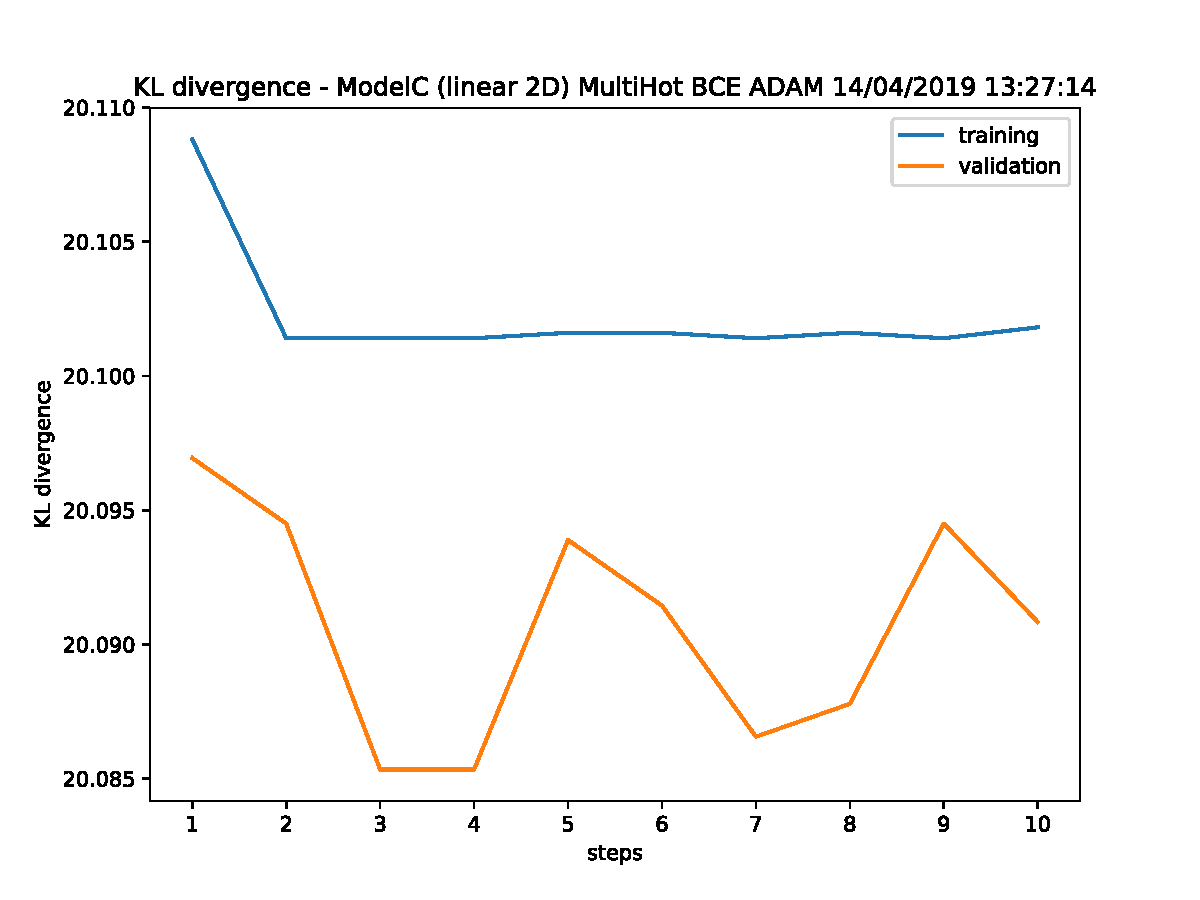
\includegraphics[width=0.48\textwidth]{figures/training_plots/ModelC-(linear_2D)-MultiHot-BCE-ADAM_14-04-2019_13-27-14_KL-divergence.pdf}
            \end{tabular}
            \caption*{Linear magnitude, multi-hot encoding, BCE loss}
        \end{figure}
        
        \begin{figure}[H]
            \centering
            \begin{tabular}{cc}
                \includegraphics[width=0.48\textwidth]{figures/training_plots/ModelC-(linear_2D)-MultiHot-KLD-ADAM_14-04-2019_18-52-21_AON-accuracy.pdf} & \includegraphics[width=0.48\textwidth]{figures/training_plots/ModelC-(linear_2D)-MultiHot-KLD-ADAM_14-04-2019_18-52-21_binary-accuracy.pdf} \\
                \includegraphics[width=0.48\textwidth]{figures/training_plots/ModelC-(linear_2D)-MultiHot-KLD-ADAM_14-04-2019_18-52-21_binary-cross-entropy.pdf} & \includegraphics[width=0.48\textwidth]{figures/training_plots/ModelC-(linear_2D)-MultiHot-KLD-ADAM_14-04-2019_18-52-21_loss.pdf}
            \end{tabular}
            \caption*{Linear magnitude, multi-hot encoding, KLD loss}
        \end{figure}
        
        \begin{figure}[H]
            \centering
            \begin{tabular}{cc}
                \includegraphics[width=0.48\textwidth]{figures/training_plots/ModelC-(log_2D)-OneHot-BCE-ADAM_05-04-2019_20-28-23_AON-accuracy.pdf} & \includegraphics[width=0.48\textwidth]{figures/training_plots/ModelC-(log_2D)-OneHot-BCE-ADAM_05-04-2019_20-28-23_categorical-accuracy.pdf} \\
                \includegraphics[width=0.48\textwidth]{figures/training_plots/ModelC-(log_2D)-OneHot-BCE-ADAM_05-04-2019_20-28-23_loss.pdf} & \includegraphics[width=0.48\textwidth]{figures/training_plots/ModelC-(log_2D)-OneHot-BCE-ADAM_05-04-2019_20-28-23_KL-divergence.pdf}
            \end{tabular}
            \caption*{Log magnitude, one-hot encoding, BCE loss}
        \end{figure}
        
        \begin{figure}[H]
            \centering
            \begin{tabular}{cc}
                \includegraphics[width=0.48\textwidth]{figures/training_plots/ModelC-(log_2D)-OneHot-KLD-ADAM_06-04-2019_08-42-01_AON-accuracy.pdf} & \includegraphics[width=0.48\textwidth]{figures/training_plots/ModelC-(log_2D)-OneHot-KLD-ADAM_06-04-2019_08-42-01_categorical-accuracy.pdf} \\
                \includegraphics[width=0.48\textwidth]{figures/training_plots/ModelC-(log_2D)-OneHot-KLD-ADAM_06-04-2019_08-42-01_binary-cross-entropy.pdf} & \includegraphics[width=0.48\textwidth]{figures/training_plots/ModelC-(log_2D)-OneHot-KLD-ADAM_06-04-2019_08-42-01_loss.pdf}
            \end{tabular}
            \caption*{Log magnitude, one-hot encoding, KLD loss}
        \end{figure}
        
        \begin{figure}[H]
            \centering
            \begin{tabular}{cc}
                \includegraphics[width=0.48\textwidth]{figures/training_plots/ModelC-(log_2D)-MultiHot-BCE-ADAM_13-04-2019_00-21-46_AON-accuracy.pdf} & \includegraphics[width=0.48\textwidth]{figures/training_plots/ModelC-(log_2D)-MultiHot-BCE-ADAM_13-04-2019_00-21-46_binary-accuracy.pdf} \\
                \includegraphics[width=0.48\textwidth]{figures/training_plots/ModelC-(log_2D)-MultiHot-BCE-ADAM_13-04-2019_00-21-46_loss.pdf} & \includegraphics[width=0.48\textwidth]{figures/training_plots/ModelC-(log_2D)-MultiHot-BCE-ADAM_13-04-2019_00-21-46_KL-divergence.pdf}
            \end{tabular}
            \caption*{Log magnitude, multi-hot encoding, BCE loss}
        \end{figure}
        
         \begin{figure}[H]
            \centering
            \begin{tabular}{cc}
                \includegraphics[width=0.48\textwidth]{figures/training_plots/ModelC-(log_2D)-MultiHot-KLD-ADAM_13-04-2019_16-30-38_AON-accuracy.pdf} & \includegraphics[width=0.48\textwidth]{figures/training_plots/ModelC-(log_2D)-MultiHot-KLD-ADAM_13-04-2019_16-30-38_binary-accuracy.pdf} \\
                \includegraphics[width=0.48\textwidth]{figures/training_plots/ModelC-(log_2D)-MultiHot-KLD-ADAM_13-04-2019_16-30-38_binary-cross-entropy.pdf} & \includegraphics[width=0.48\textwidth]{figures/training_plots/ModelC-(log_2D)-MultiHot-KLD-ADAM_13-04-2019_16-30-38_loss.pdf}
            \end{tabular}
            \caption*{Log magnitude, multi-hot encoding, KLD loss}
        \end{figure}
        
    \newpage
    \section{Confusion matrices}
        \subsection{Model A}
        \label{app:modelA_confusion_matrix}
        \texttt{Referred to in section \ref{sec:evaluation_analysis_modelA}}
            \begin{figure}[H]
                \centering
                \includegraphics[width=\textwidth]{figures/confusion_matrices/ModelA-(1D)-OneHot-BCE-ADAM_10-04-2019_10-36-18.pdf}
                \caption*{Model A with one-hot encoding and BCE loss. This model got:  68.62\% $Acc_{AON}$ and left 25.69\% of test data unclassified.}
            \end{figure}
            
            \begin{figure}[H]
                \centering
                \includegraphics[width=\textwidth]{figures/confusion_matrices/ModelA-(1D)-OneHot-KLD-ADAM_10-04-2019_18-45-24.pdf}
                \caption*{Model A with one-hot encoding and KLD loss. This model got:  69.30\% $Acc_{AON}$ and left 24.11\% of test data unclassified.}
            \end{figure}
            
            \begin{figure}[H]
                \centering
                \includegraphics[width=\textwidth]{figures/confusion_matrices/ModelA-(1D)-MultiHot-BCE-ADAM_12-04-2019_07-48-00.pdf}
                \caption*{Model A with multi-hot encoding and BCE loss. This model got:  52.53\% $Acc_{AON}$ and left 19.77\% of test data unclassified.}
            \end{figure}
            
        \newpage
        \subsection{Model B}
        \label{app:modelB_confusion_matrix}
        \texttt{Referred to in section \ref{sec:evaluation_analysis_modelB}}
            \begin{figure}[H]
                \centering
                \includegraphics[width=\textwidth]{figures/confusion_matrices/ModelB-(1D)-OneHot-BCE-ADAM_07-04-2019_02-15-18.pdf}
                \caption*{Model B with one-hot encoding and BCE loss. This model got:  81.53\% $Acc_{AON}$ and left 12.74\% of test data unclassified.}
            \end{figure}
            
            \begin{figure}[H]
                \centering
                \includegraphics[width=\textwidth]{figures/confusion_matrices/ModelB-(1D)-OneHot-KLD-ADAM_13-04-2019_11-59-08.pdf}
                \caption*{Model B with one-hot encoding and KLD loss. This model got:  83.80\% $Acc_{AON}$ and left 12.38\% of test data unclassified.}
            \end{figure}
            
            \begin{figure}[H]
                \centering
                \includegraphics[width=\textwidth]{figures/confusion_matrices/ModelB-(1D)-MultiHot-BCE-ADAM_12-04-2019_19-00-30.pdf}
                \caption*{Model B with multi-hot encoding and BCE loss. This model got: 50.67\% $Acc_{AON}$ and left 21.89\% of test data unclassified.}
            \end{figure}
            
        \newpage
        \subsection{Model C}
        \label{app:modelC_confusion_matrix}
        \texttt{Referred to in section \ref{sec:evaluation_analysis_modelC}}
            \begin{figure}[H]
                \centering
                \includegraphics[width=\textwidth]{figures/confusion_matrices/ModelC-(linear_2D)-OneHot-KLD-ADAM_13-04-2019_21-26-52.pdf}
                \caption*{Model C using linear spectrogram input with one-hot encoding and KLD loss. This model got:  0.69\% $Acc_{AON}$ and left 0.00\% of test data unclassified.}
            \end{figure}
            
            \begin{figure}[H]
                \centering
                \includegraphics[width=\textwidth]{figures/confusion_matrices/ModelC-(linear_2D)-MultiHot-BCE-ADAM_14-04-2019_13-27-14.pdf}
                \caption*{Model C using linear spectrogram input with multi-hot encoding and BCE loss. This model got:  0.93\% $Acc_{AON}$ and left 0.00\% of test data unclassified.}
            \end{figure}
    
            \begin{figure}[H]
                \centering
                \includegraphics[width=\textwidth]{figures/confusion_matrices/ModelC-(log_2D)-OneHot-BCE-ADAM_05-04-2019_20-28-23.pdf}
                \caption*{Model C using log spectrogram input with one-hot encoding and BCE loss. This model got: 62.64\% $Acc_{AON}$ and left 29.06\% of test data unclassified.}
            \end{figure}
            
            \begin{figure}[H]
                \centering
                \includegraphics[width=\textwidth]{figures/confusion_matrices/ModelC-(log_2D)-OneHot-KLD-ADAM_06-04-2019_08-42-01.pdf}
                \caption*{Model C using log spectrogram input with one-hot encoding and KLD loss. This model got: 00.64\% $Acc_{AON}$ and left 0.00\% of test data unclassified.}
            \end{figure}
            
            \begin{figure}[H]
                \centering
                \includegraphics[width=\textwidth]{figures/confusion_matrices/ModelC-(log_2D)-MultiHot-BCE-ADAM_13-04-2019_00-21-46.pdf}
                \caption*{Model C using log spectrogram input with multi-hot encoding and BCE loss. This model got: 46.91\% $Acc_{AON}$ and left 10.67\% of test data unclassified.}
            \end{figure}
    
\end{appendices}
